\section{Implementation}\label{Section:Implementation}
Web applications provide a way of delivering a system to multiple users across multiple devices rather than creating a separate application tailored to each platform. A single backend powers the application across all devices which reduces the work for the developer and makes maintenance of the application simpler. In addition, web applications provide a simple interface for interacting with a range of other technologies such as MySQL and file servers. With the popularisation of this technique in recent years, various frameworks such as Bootstrap and Laravel have been developed, allowing the developer to rapidly prototype and deliver applications to their users. One obvious requirement of such a system is a connection to the internet. Considering all these facts, a web application seems like a sensible approach for the system being proposed.

\subsection{Technologies}
Numerous technologies were employed to build the end product. These are categories into storage, processing and visualisation depending on the purpose they server. Discussion of the final selections such as MySQL, PHP and HTML-CSS are given in the section below based on the research conducted in section \ref{Section:Research}.

\subsubsection{Storage}
MySQL is an open source database management system used for managing data held in a relational database management system \cite{MySQL:Home}. It is the world's most popular open source database. The RDMBS is written in C and C++ and has been extensively tested which ensure that it is stable. Many of the world's largest and fastest-growing organisations including Facebook, Google, Adobe, Alcatel Lucent and Zappos rely on MySQL to save time and money powering their high-volume Web sites, business-critical systems and packaged software \cite{MySQL:Home}. 

The reasons behind the use of MySQL database are vast but the key factor is the ease with which a MySQL database can be setup and migrated. MySQL databases have existed for a long time which means overtime they have been improved and now guarantee stability, scalability and security \cite{MySQL:Why}. The long life of MySQL database systems also means that a wide range of third-party party tools are available to the developer for working with and processing the data. In addition to a MySQL database, a fileserver is being used to store files that may be uploaded as resources.

\subsubsection{Processing}
Majority of the data processing will be done using the popular server sided scripting language PHP. All PHP scripts are executed on the server which may produce output that can be presented to the user. The language is used by millions of websites available on the internet and has for some time been the hottest scripting language for dynamic web development. This wide adoption of the PHP scripting language has allowed extensive libraries and frameworks to be made available and used for rapid development of web applications. Laravel is an example of a Framework that is a result of years of development and will be used to provide a model-view-controller approach for the system.

PHP has shown to be scalable as it is powerful enough to be at the core of the biggest blogging system on the web, known as WordPress, but at the same time it is deep enough to run the largest social network, Facebook\cite{W3Schools:PHP_Intro, Wiki:WordPress, Fastcompany:Facebook_PHP}. This means that in the future if the system is to grow large enough, it can easily be scaled as done so over time by the aforementioned examples. In addition to PHP, JavaScript will be used for some client sided data processing along with SQL which will be used to process data from the database before it is retrieved.

\subsubsection{Visualisation}
HTML is being used to define structure of the pages on the website whereas CSS is being used to design the components on the page \cite{W3:HTML5, W3:CSS}. In addition to this, the Laravel blade engine is being used to make the generation of pages easier by splitting content up into views that can be extended by  or rendered inside other views \cite{Laravel:Blade}. This encourages good practices by abstracting the system and enforcing modularity throughout. This allows development in the future to continue where new components can easily be added and master views can easily be replaced to change the appearance across the system. Technologies such as Google Maps and Bootstrap are also being employed to make the pages more dynamic by providing visual interaction.

\subsection{Installation and Setup}
Many of the technologies being employed are not included by default on an ordinary machine. Thus, before development could be initiated, it was necessary to install and configure the required technologies. This section details the technologies that were configured as well as the process and any other prerequisites.

\subsubsection{Initial Setup}
In order to develop and test the system, it was necessary to install an Apache web server capable of interpreting php and rendering web pages. In addition to this, an SQL server was required to host the MySQL database. The solution for this was a package known as XAMPP which provides an SQL and a web server in one setup. These are automatically configured by the XAMPP package upon installation and immediately ready to use out of the box. The server could be booted up using a simple control panel and accessed using \emph{http://localhost/} at any time. Any files can them be placed inside the htdocs folder, created during the installation process, and are immediately made available. 

\subsubsection{IDE and Laravel}
The project is built using the Laravel framework but this is not readily available for download as an archive like most other frameworks. In order to install the Laravel framework, a package manager known as composer was used. Once installed a new project could be created using the command \emph{laravel new Frisk}. This creates a new directory names Frisk with all the required files and dependencies. Updates and additional packaged may be installed using composer and the included JSON file.

Development could be carried out using a simple text editor but better and more efficient tools exist which speed up the process of writing code. The PhpStorm IDE by JetBrains was used throughout the entire development process as it provides features such as code suggestion and error detection. Unfortunately, the IDE is not fully compatible with the Laravel and additional plugins had to be installed to make use of some of the features.

\subsection{Database}
The database is at the core of the application and thus care must be taken when setting up and configuring the database. A range of tools, provided by Laravel, were employed for configuring and interacting with the database. Details of the configuration and setup are discussed in detail.

\subsubsection{Configuration}
All interaction with the database occurs through models, the query builder, the schema builder and migrations provided as part of the Laravel framework. Settings inside the projects configuration file need to be tweaked in order for these components to function correctly. These settings allow the developer to change the connection, authentication and driver details for the application. In this project setup the PDO driver was used to connect to the database. Figure \ref{fig:Database_Config} shows some of the settings that may be tuned in the configuration file.

\begin{figure}[H]
	\centering
	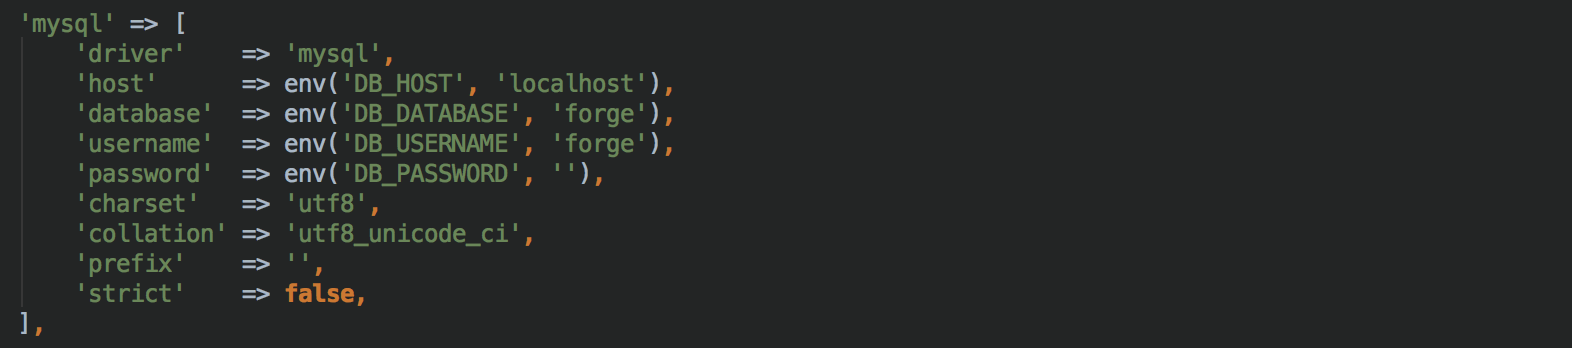
\includegraphics[width=1.0\textwidth]{images/Code/Database_Config}
	\caption{Database Configuration for MySQL Databases} \label{fig:Database_Config}
\end{figure}

\subsubsection{Migrations}
"Migrations are like version control for your database, allowing a team to easily modify and share the application's database schema" \cite{Laravel:Migrations}. The use of migrations not only allows for the database to be replicated anywhere the system is installed with ease but also simplifies the process of updating an existing table during the development process.  To create a migration, one can use the \emph{make:migration} command provided by the Laravel Artisan utility.

\begin{lstlisting}[language=bash]
	$ php artisan make:migration create_users_table  --create=Users
\end{lstlisting}

The command shown above generates an empty template for the specified table name. When creating a new table, the \emph{--create} argument is used whereas the \emph{--table} argument is used for modifying an existing table. The generated template contains an \emph{up} method, used for adding new columns and index, and a \emph{down} method which reverses the changes produced by the \emph{up} method. Migrations are typically paired with Laravel's schema builder to easily build your application's database schema \cite{Laravel:Migrations}. The schema builder can be used to define the schema for the table using calls to php functions. Once the schema has been populated, the \emph{migrate} command can be used to run the migration and update the database. In the case of an error the users can revert to a previous version of the database using the \emph{migrate:rollback} command. It is always encouraged that major changes, such as adding new columns and adding indexes, are introduced using new migrations rather than rolling back and updating existing migrations. All database tables were created using Laravel migrations and are available in the code.

\begin{figure}[H]
	\centering
	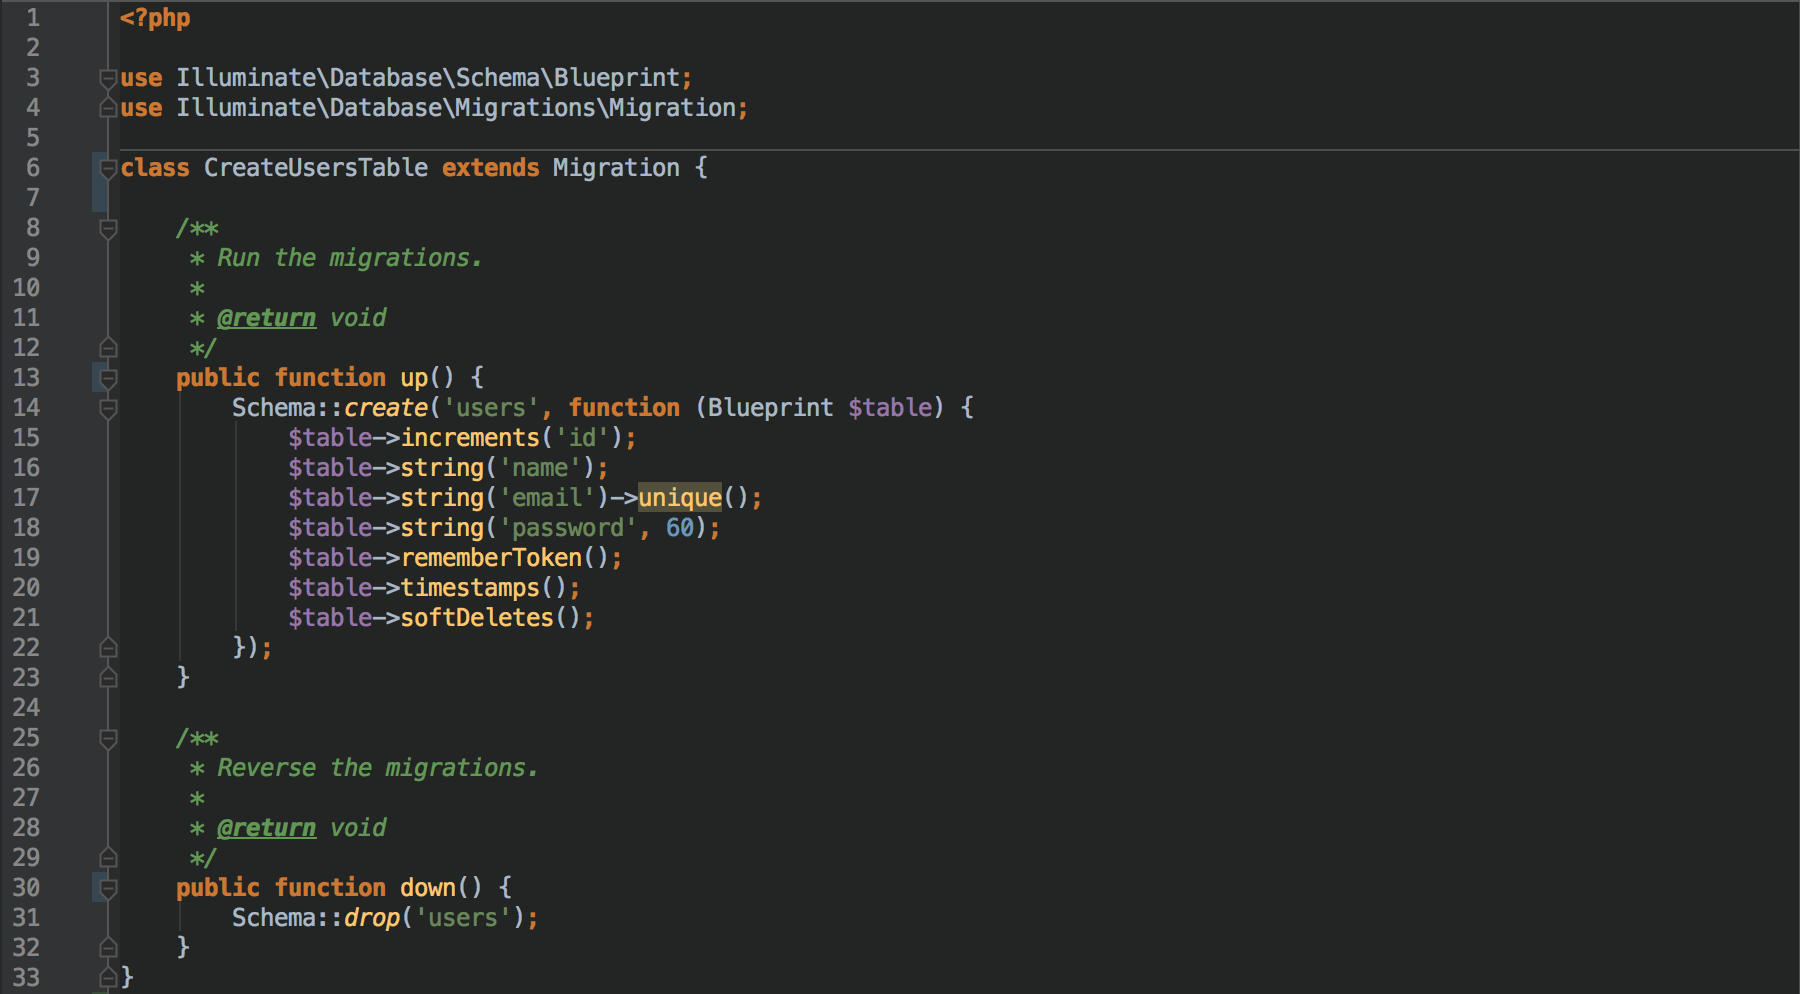
\includegraphics[width=1.0\textwidth]{images/Code/Migration_Users}
	\caption{Migration for Creating Users Table} \label{fig:Migration_Users}
\end{figure}

Figure \ref{fig:Migration_Users} shows the migration for the users table which was used for authentication. The migration in the figure is the final schema for the production database rather than being spread out across several migrations as the schema was changed. As visible in the image, the schema builder can be used in the up method to define the structure of the table. Each migration schema contains an \emph{id} field, generated by calling the \emph{increments} method, and the \emph{create\_at} and \emph{updated\_at} timestamp, generated by calling the \emph{timestamps} method, by default. The \emph{increments} method is used for assigning an auto incrementing primary key, discussed later in the report, used for associating record through relationships. A \emph{deleted\_at} timestamp was added to all tables by calling the \emph{softDeletes} method. A range of other method such as \emph{string} and \emph{integer} can be used for creating more attributes. A full list of operations is available in the Laravel documentation \cite{Laravel:Migrations}. 

The code shown in figure \ref{fig:Migration_Users} provides an introduction to the workings of the schema builder and migrations. The two together may be used to create a table with any complex sql operations. For example, referential constraints can be added using simple method calls as shown in figure \ref{fig:Referential_Constraints}.

\begin{figure}[H]
	\centering
	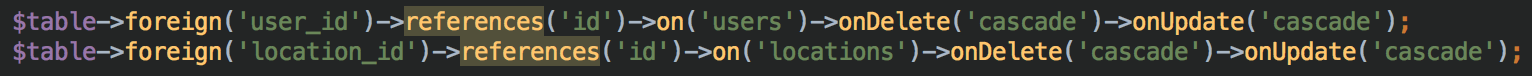
\includegraphics[width=1.0\textwidth]{images/Code/Referential_Constraints}
	\caption{Referential Constraints using Schema Builder and Migrations} \label{fig:Referential_Constraints}
\end{figure}

\subsubsection{Association}
The data in the system must always be associated with something or someone for it to hold any meaning. This is also one of the requirements for the system and thus holds even more importance. Linking data to a user through their email address or other personally identifiable information can lead to security issues. To combat this problem, unique IDs were used for all records inserted into any of the tables in the database. These IDs are generated by creating an auto incrementing integer field in the table which is automatically assigned when a row is inserted into with a NULL value for the auto incrementing attribute. There can only be one auto incrementing attribute in the database and this is assigned as the primary the key.

A primary key is a special relational database table column (or combination of columns) designated to uniquely identify all table records \cite{Techopedia:Primary_keys}. Naturally, in order to identify each record in the table, the primary key must contain a unique value for each row of data and it cannot be null. These primary IDs can then be used as pointer to associate one entity to another.

\subsubsection{Querying}
Laravel makes running queries extremely simple using either raw SQL, the fluent query builder, and the Eloquent ORM. \cite{Laravel:Database}. For most part the Eloquent ORM approach was used to retrieve the result from the database but the approaches have been used in rare cases. All three approaches are outlined below.

\paragraph{Raw SQL}
Using raw SQL in Laravel is extremely straight forward using the built in classes. There is no need to open a connecting to the database, create statements and bind parameters as there are all done automatically. For example, as shown in the example below, the user can run an SQL query to retrieve a user with a specific ID of 1 just by using the \emph{DB::select} method.

\begin{lstlisting}[language=php]
	$users = DB::select('SELECT * FROM users WHERE id = ?', [1]);
\end{lstlisting}

The above query will return an array of objects modelling the users entity in the database. The developer can then loop through the array and access the properties of each user as \emph{\$user-$>$property}, where property may be any attribute such as fullName or email.

\paragraph{Query Builder}
The database query builder provides a convenient, fluent, and easy to use interface for creating and executing database queries \cite{Laravel:QueryBuilder}. The query builder can perform most operations supported by the database driver. One of the main advantages of the Laravel query builder is that it uses PDO parameter binding for preventing SQL injection which means there is no need to sanitise user input. Using the query builder, one could retrieve the user with ID 1 by executing the following statement.

\begin{lstlisting}[language=php]
	$user = DB::table('users')->where('id', 1)->first();
\end{lstlisting}

The above query would fetch the result where the user id matches 1 and retrieve the first result. Once again, the result is returned as an object modelling the entity and the properties can be accessed as \emph{\$user-$>$property} but this time there is no need to loop through the result as only one result is returned.

\paragraph{Eloquent Object-Relational Mapping}
The Eloquent Object-Relational Mapping (ORM) included with Laravel provides an simple and elegant activeRecord implementation for working with the database \cite{Laravel:Eloquent}. "Object-relational mapping (ORM) is a mechanism that makes it possible to address, access and manipulate objects without having to consider how those objects relate to their data sources" \cite{TechTarget:ORM}. Each database table has a corresponding "Model" which is used to interact with the database and more specifically the table. The model allows the developer to query, insert, update, and delete records in the corresponding table as well as more complex operations such as joining tables. When the user queries the database using a model, Eloquent automatically instantiates and maps a model for each row in the result allowing the developer to utilise the models behaviour.

\begin{lstlisting}[language=bash]
	$ php artisan make:model Models/User
\end{lstlisting}

Creating a model is extremely simple using the Artisan utility, shipped with the Laravel installation. The command above will generate a User model in the \emph{app/Models} directory. Each Eloquent models extends the \empty{Illuminate/Database/Eloquent/Model} class which utilises the query builder for all interactions \cite{Laravel:Eloquent}. By default, Eloquent assumes that each table has a primary key field named \emph{id} and the \emph{created\_at} and \emph{updated\_at} timestamps but these can all be changed by toggling optional properties in the model. In order to use a model, the developer simply needs to import the model in the controller where it will be used. The user can simple execute the following command in order to retrieve the user with id 1.

\begin{lstlisting}[language=php]
	$user = User::find(1);
\end{lstlisting}

The line of code above will return the \emph{User} model with all the attributes populated from the values in the database. The user can then access these properties as \emph{\$user-$>$property}. The main change to be noticed here is that the user can actually update the properties and then append these updates to the database by simply calling \emph{\$user-$>$save()} \cite{Laravel:Eloquent}.  The image in figure \ref{fig:Model_User} shows the code for the User model. As visible in the image, it is possible to add custom methods to the model which may be called when the model is returned as a result.

\begin{figure}[H]
	\centering
	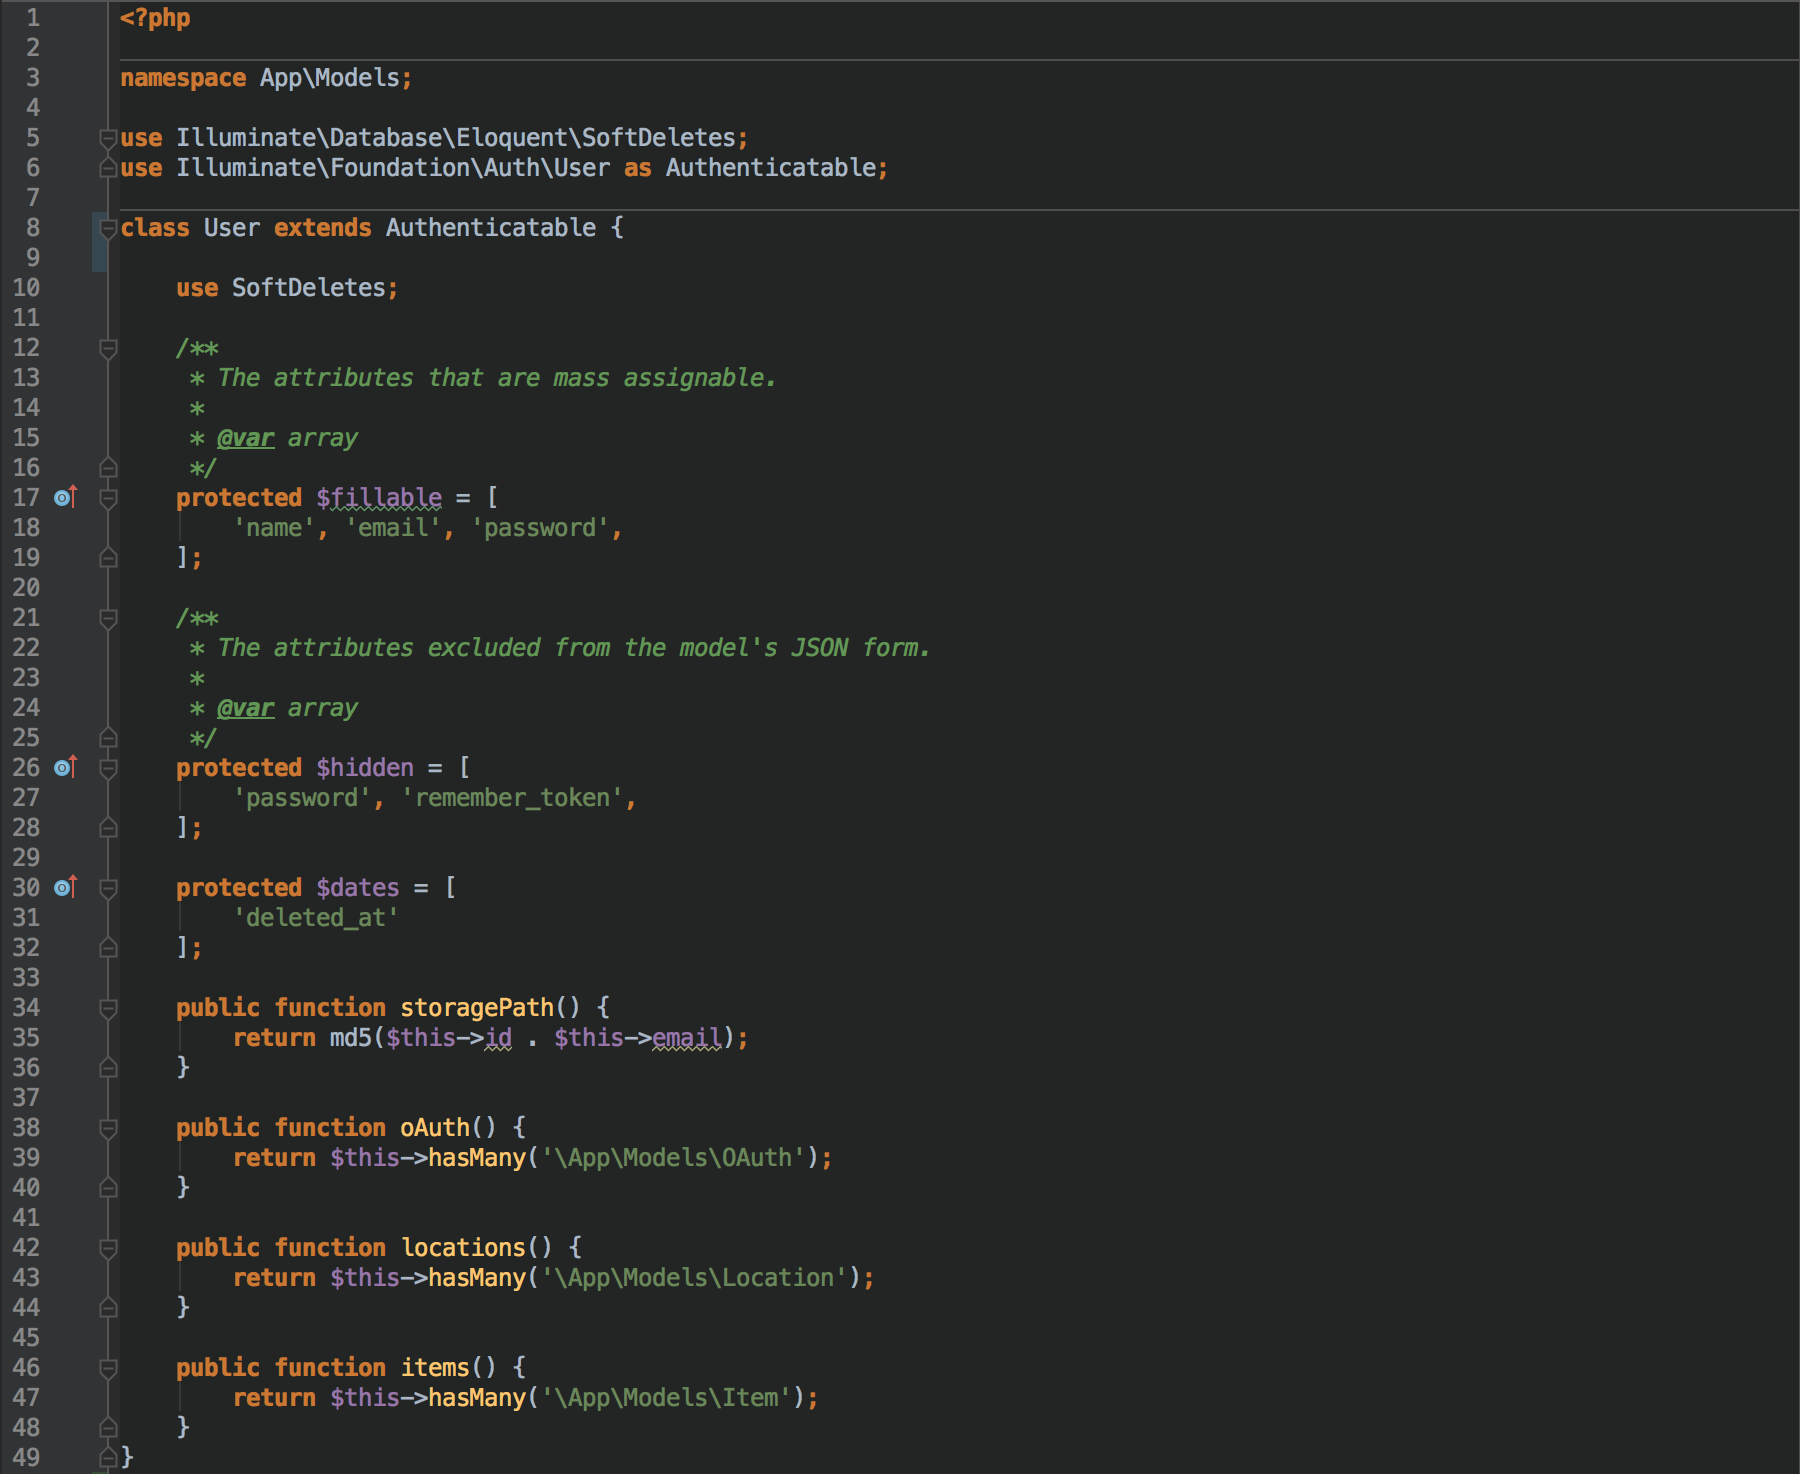
\includegraphics[width=1.0\textwidth]{images/Code/Model_User}
	\caption{Users Eloquent Object-Relational Mapping Model} \label{fig:Model_User}
\end{figure}

\subsection{Routing and Middleware}
Laravel allows the developer to define custom routes in contract to the normal approach where routes are determined by the URI of the page. In addition, Laravel allows for filtering of HTTP requests through the use of middleware. Both of these approaches, used for implementing user friendly URLs and security, are discussed in this section.

\subsubsection{Routes}
All routes for the application are defined inside the \emph{app/Http/routes.php} file which is automatically loaded by the framework \cite{Laravel:Routing}. The easiest way to define a route in Laravel is by passing a URI and a closure which is executed when the URI is hit. However, this approach limits the functionality of the application and instead we can pass the name of a controller followed by the name of the method which is to be called if a URI is hit. Routes can be grouped together if they share common features of functionality. For example, all the routes are contained within the default 'web' middleware group, which provides access to session state and CSRF protection \cite{Laravel:Routing}.

\begin{figure}[H]
	\centering
	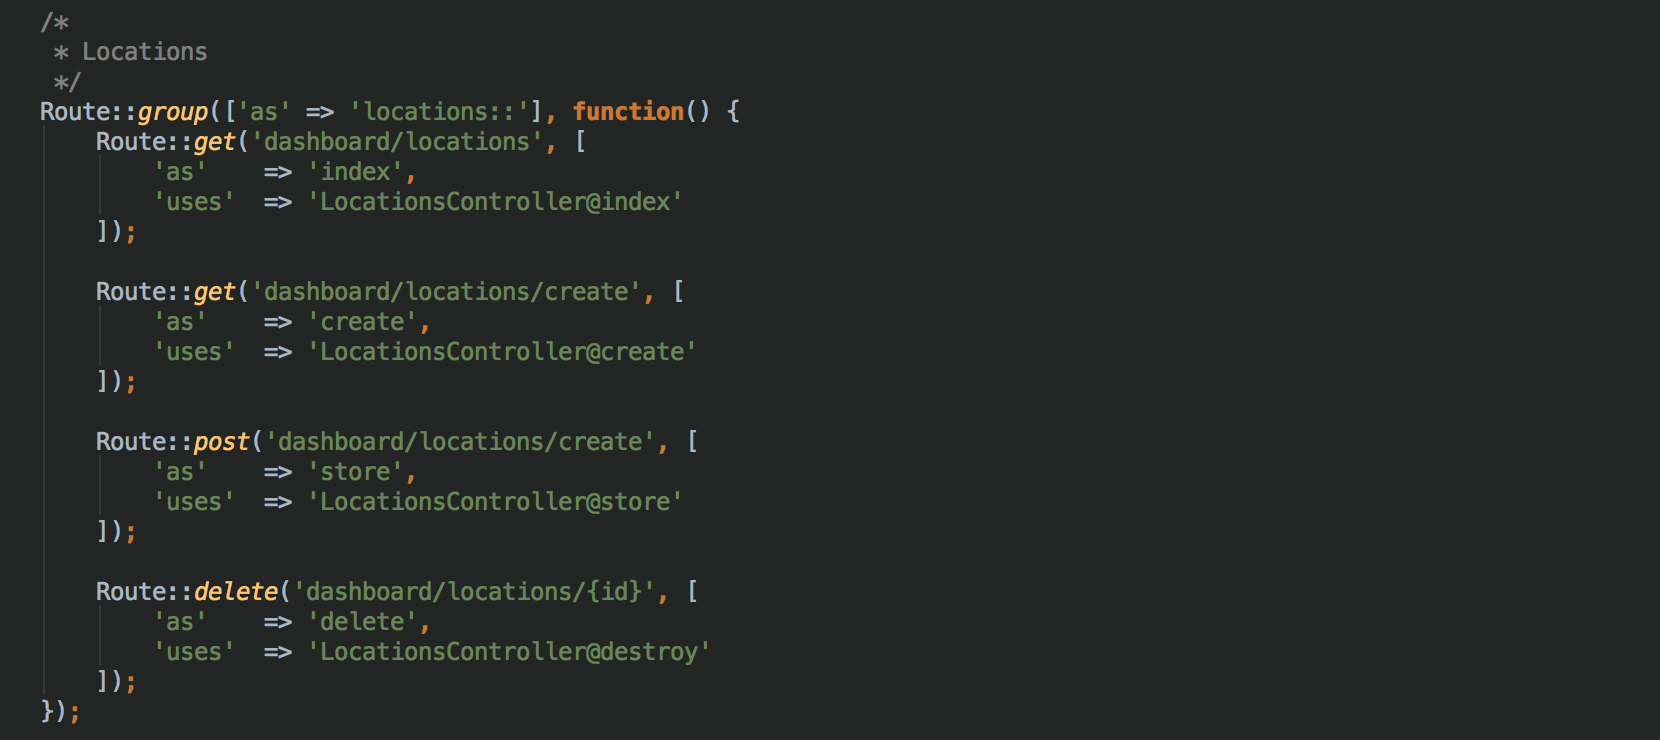
\includegraphics[width=1.0\textwidth]{images/Code/Routes}
	\caption{Routes Defined in the Locations Group} \label{fig:Routes}
\end{figure}

Figure \ref{fig:Routes} shows the code which defines all the routes regarding the locations component in the dashboard. The routes are grouped together with a prefix using the \emph{'as'} parameter. This adds the 'locations::' prefix to the name of each route. For example, using \emph{route('locations::index')} will generate the URL pointing to the index page for locations. Parameters may additionally be requested for each route which can be passed to the \emph{route()} method when generating URLs and allow for more flexible URLs. This is shown for the delete route in figure \ref{fig:Routes} where \ref{id} is a required parameter and is automatically passed to the destroy method in the controller when the URL is hit.

Security is achieved using routes by restricting each route to a certain type of request. Laravel provides get, post, put, patch, and delete options for each route. A route defined using \emph{route::post} may only be accessed if the user posts form data to the URL. It is possible to bind a route to multiple request types such as get and post or even all request types but this is not recommended.

\subsubsection{Middleware}
HTTP middleware provide a convenient mechanism for filtering HTTP requests entering your application \cite{Laravel:Middleware}. Middleware are generally executed before the page is loaded in order to assess whether the user can access the page. It is possible for a page to have multiple middleware and this can be though of as a chain of middleware, where passing the requirements for one leads to the next one being called. A middleware can be assigned to a route, method, a controller or even a group of middleware.

\begin{lstlisting}[language=bash]
	$ php artisan make:middelware Demo
\end{lstlisting}

 It is possible to create custom middleware using the Artisan utility. The command above will generate a middleware called Demo. The image in figure \ref{fig:Middleware_Template} shows the template that is generated by the Artisan utility. The commented block on line 17 can be replaced with a check, which if passed allows the next middleware to be activated but if failed returns an alternative action to be executed. Middleware were used in to achieve several trivial tasks in the application and each is discussed separately throughout the implementation section.


\begin{figure}[H]
	\centering
	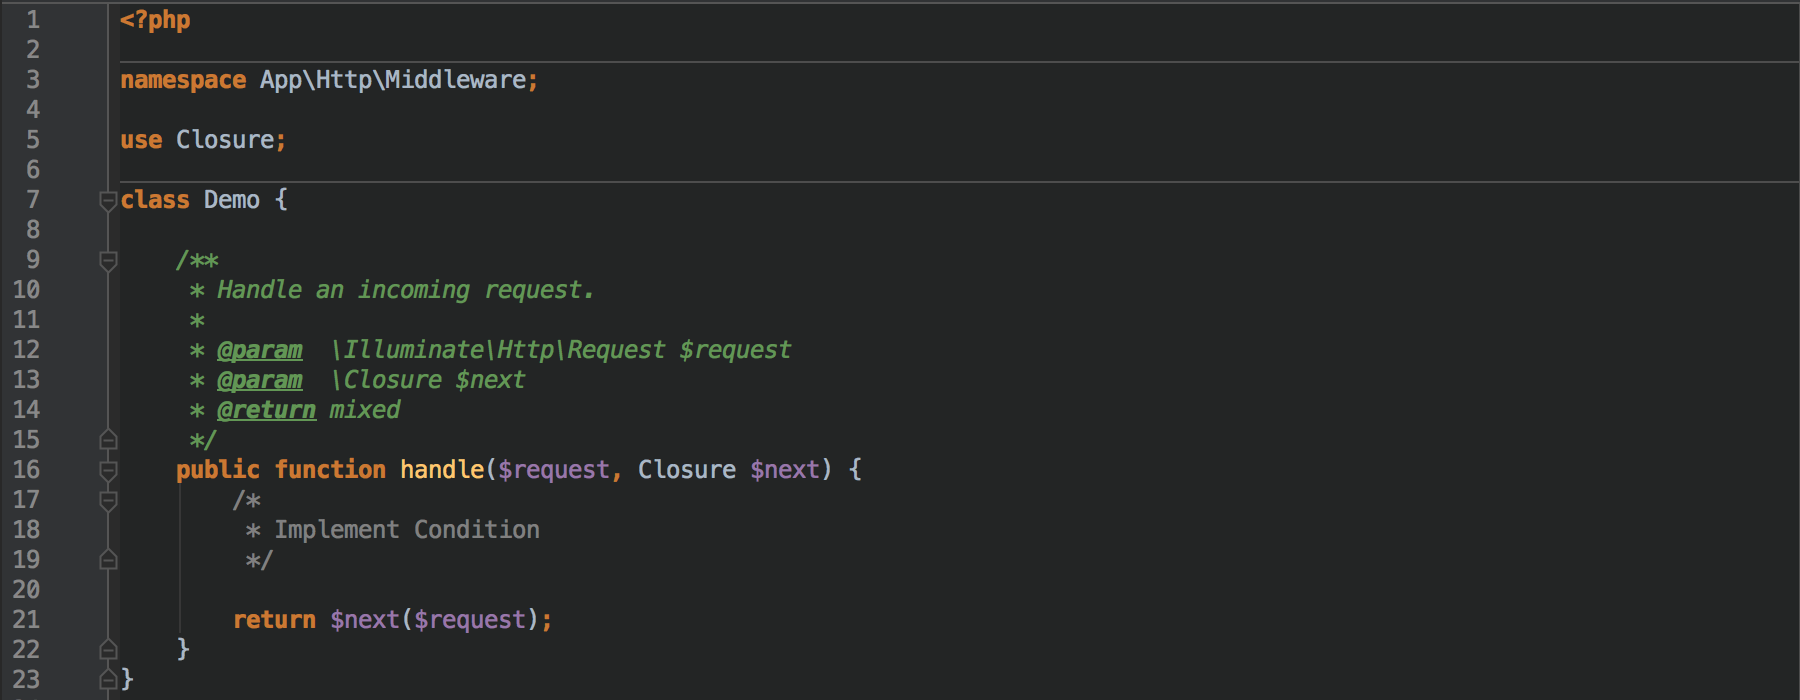
\includegraphics[width=1.0\textwidth]{images/Code/Middleware_Template}
	\caption{Middleware Template Generated by the Artisan Utility} \label{fig:Middleware_Template}
\end{figure}

\subsection{Authentication}
Without the contribution of data by the user the system would serve no purpose and be rendered completely useless. For users to be able to add content to the system an authentication system is required which ca be used to not only allow filtered access to members but also associate data with members. Two separate forms of authentication were provided, manual and socialite authentication using oAuth. In order to provide a consistent experience across the system, a user model has been created which encapsulates any information available about  a user and 

\subsubsection{Manual Registration}
\begin{figure}[H]
	\centering
	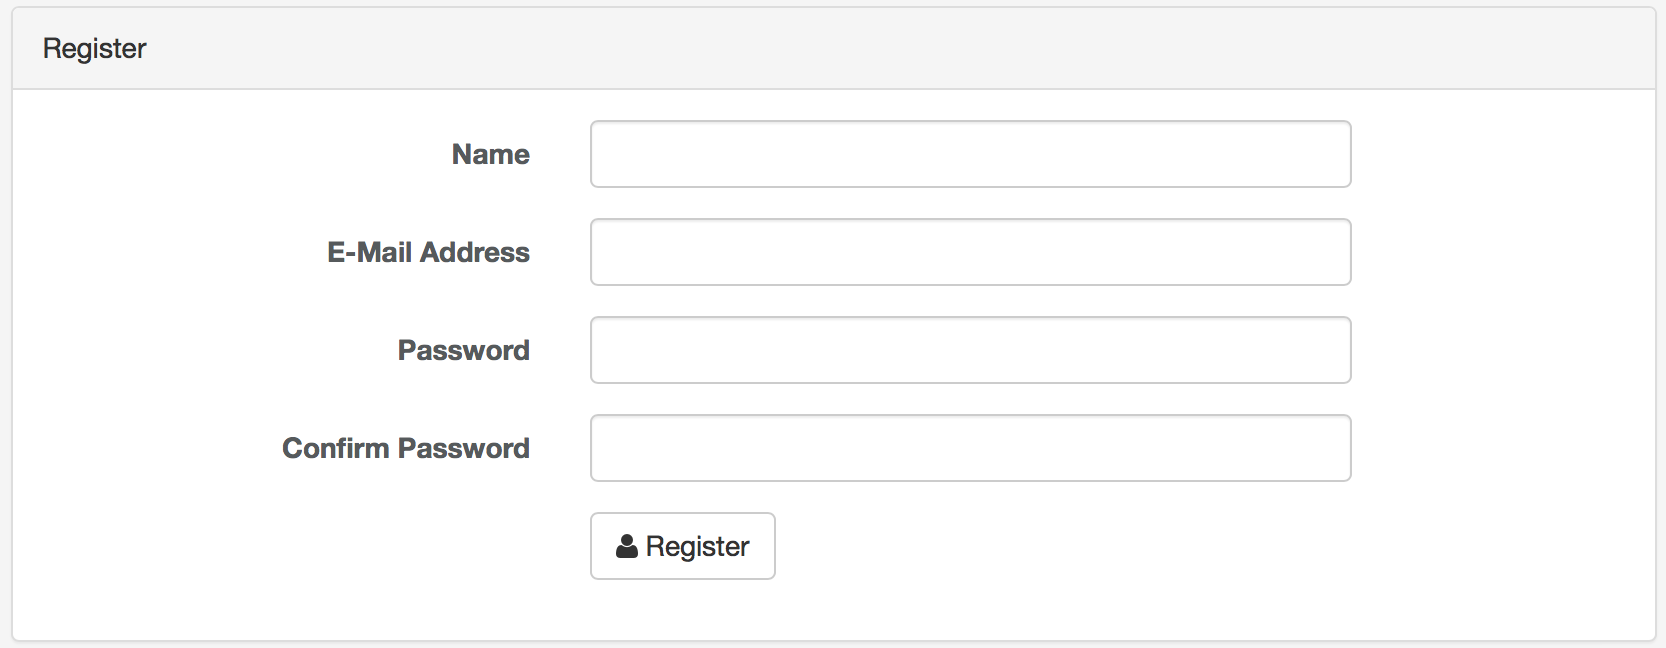
\includegraphics[width=1.0\textwidth]{images/Frisk/Registration_Form}
	\caption{Registration Page and Form} \label{fig:Registration_Form}
\end{figure}

The user is able to manually register an account by providing all the details required using the registration form (see figure \ref{fig:Registration_Form}). The form requires the user to input their full name, email address and password before continuing. An additional field is included which asks the user to confirm their password to prevent typing errors.

\begin{figure}[H]
	\centering
	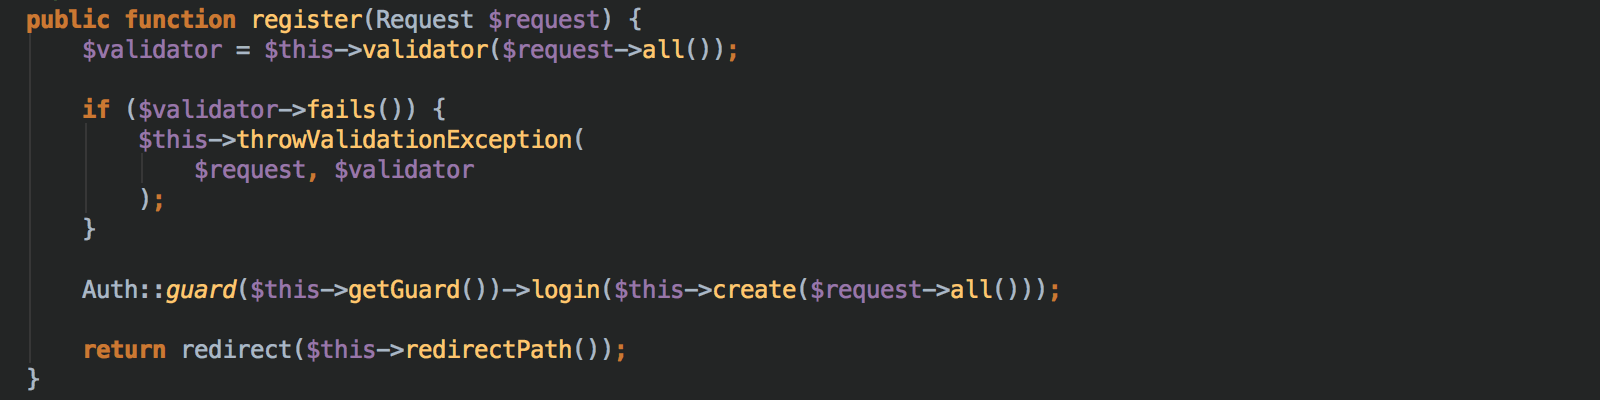
\includegraphics[width=1.0\textwidth]{images/Code/Register}
	\caption{Method for Validating and Storing Registration Data} \label{fig:Registration_Code}
\end{figure}

Once the form is completed by the user, and submitted to the \emph{register} method in the \emph{AuthController}, it is validated to make sure the data is valid. If the validation fails then the system throws an exception which causes the user to be redirected back to the registration page, which is pre-populated with the information they had previously input, but this time errors are displayed to the user. If the validation passes then the users password is hashed using the \emph{bcrypt} library provided within PHP. The hash of the password, instead of the actual plain text password, along with the other user data is then inserted into the database. Additional fields in the model which include id, create\_at, updated\_at, and deleted\_at are automatically populated by either the RDBMS or the Eloquent model. Once successfully stored, the user is then logged into the newly created account and redirect back to the homepage.

\subsubsection{Socialite Authentication}
In addition to typical, form based authentication, Laravel also provides a simple, convenient way to authenticate with OAuth providers such as Facebook, Twitter and Google using Laravel Socialite \cite{Laravel:Authentication}. OAuth 2.0 is a delegation protocol, a means of letting someone who controls a resource allow a software application to access that resource on their behalf without impersonating them \cite{OAuth2inAction}. The application requests limited authorisation from the owner of the resource and receives a token that it can use to access the resource.

\begin{figure}[H]
	\centering
	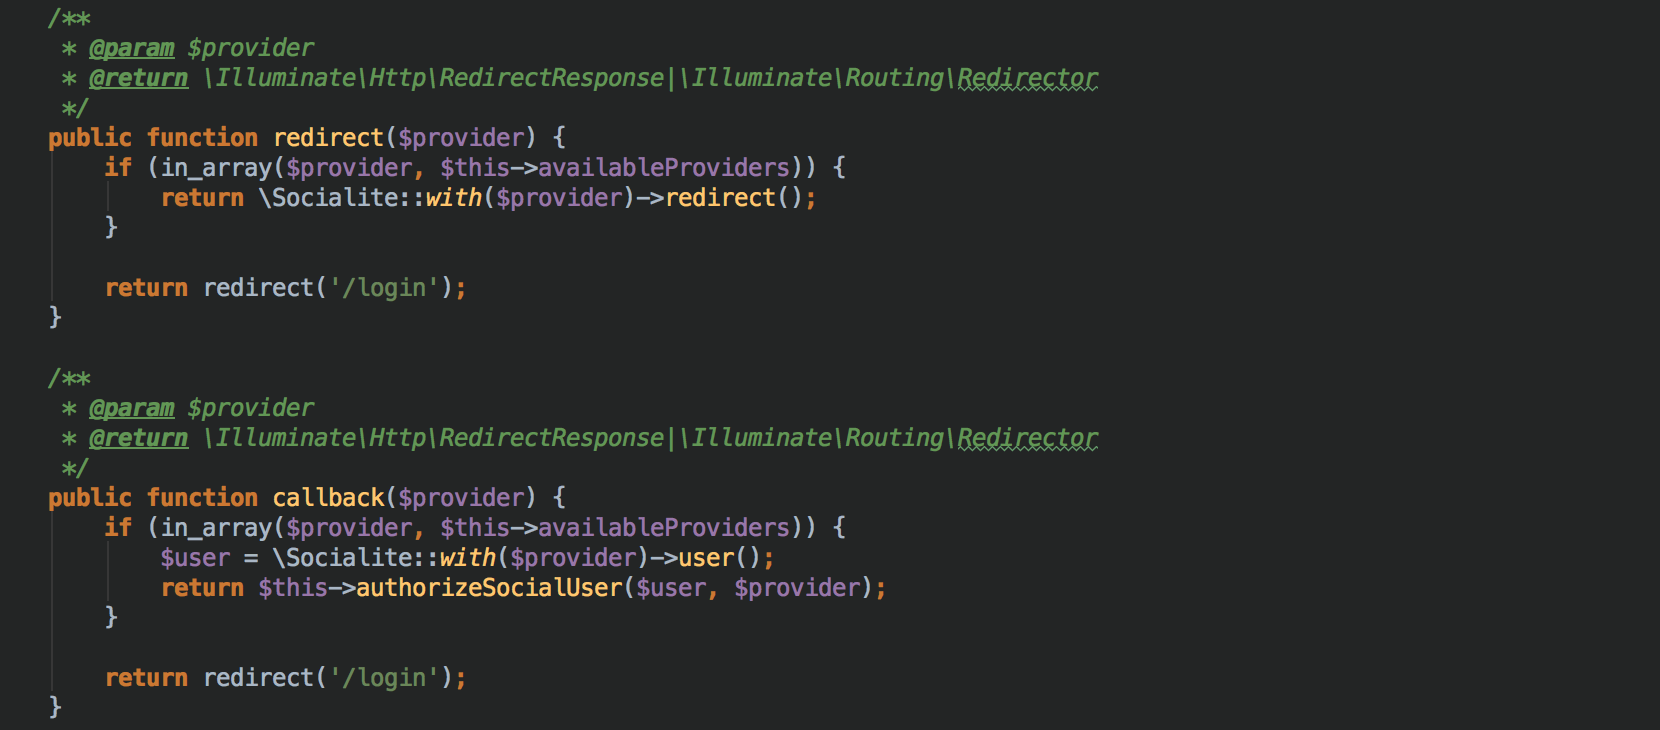
\includegraphics[width=1.0\textwidth]{images/Code/Socialite_Routes}
	\caption{Restricting Socialite Authentication to Specific Providers} \label{fig:Socialite_Routes}
\end{figure}

Although socialite supports many third-parties for authenticating using oAuth, only Google and Facebook were actually enabled. This is because they are these two along with Twitter are the three most popular choices. Unfortunately Twitter was not enabled as it does not allow access to the users email address which is an important requirement for communication with the user. Figure \ref{fig:Socialite_Routes} shows the two methods that which allowed a provider to specified as a parameter in the URL rather than having separate methods for each provider. The methods check the provider against a collection of available providers and if a match is not found then the user is redirected back to the login page. If a match is found then user is redirected to the third-party website where they must allow the application access to the required information. Once the user grants access, they are then redirected back to the application where the details are used to either authenticate an existing account or register a new account.

\begin{figure}[H]
	\centering
	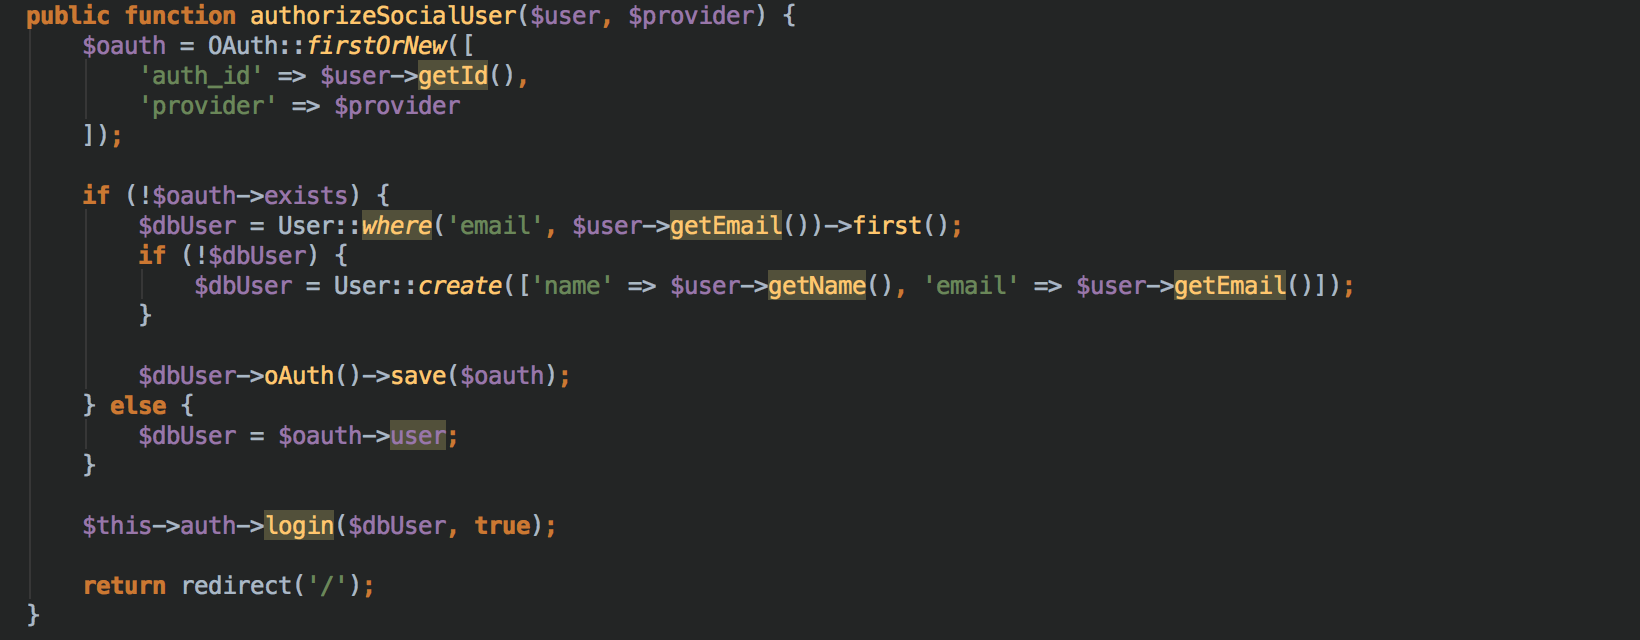
\includegraphics[width=1.0\textwidth]{images/Code/Socialite_Authorise}
	\caption{Authentication or Registering Users Using Socialite} \label{fig:Socialite_Authorise}
\end{figure}

As some users may register manually whereas other may register through oAuth, adding attributes in the users table to store the auth tokens would result in redundant fields. Additionally, one user may end up with multiple account from the various services. This would be an inefficient use of of the database storage and would break the normalisation process previously carried out. As a result, another table was created to store the oAuth tokens which were then linked to a user using the user id. This meant that if a user signed up with one service, be it manually or socialite, they'd be able to access the same account using all the other services, provided the email address was the same. Figure \ref{fig:Socialite_Authorise} shows the code that was written to achieve this. 

In order authenticate the user we can check to see if an oAuth entry exists for the user id returned by the third party and the service. If an entry exists then we simply find the user associated with the record and authenticate them. Alternatively, if an entry is not found then a new entry is created but not yet stored. Next, a check is carried out to see if the user with the given email address exists. If the user does not exist then a new user is created with the given details. Once the user has either been found or created, the oAuth record is inserted and linked to the user. Finally, the user can now be authenticated and redirect to the homepage.

\subsubsection{Manual Login}
The login page consists of the universal navigation bar which is available across all pages and a login form. The login form has two key fields which are required should the user choose manual authentication. There is also a remember me checkbox which can be ticked to keep the user logged in until they clear their browser data or manually logout. Checking the remember me box results in a unique token being generated which is stored in the database and in a cookie on the users computer so that the user can be re-authenticated when the session expires. A 'forgot?' link is also provided to the user which can be used to recover forgotten password.

\begin{figure}[H]
	\centering
	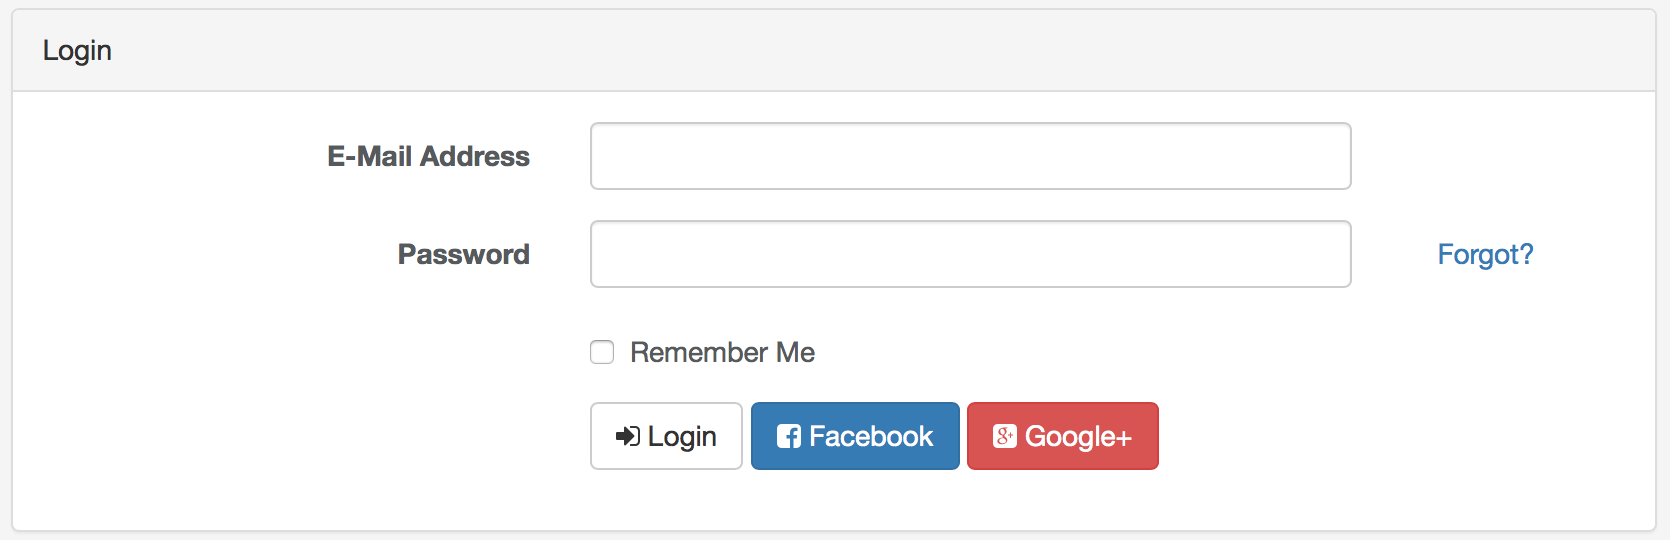
\includegraphics[width=1.0\textwidth]{images/Frisk/Login_Form}
	\caption{Login Page with Login Form and Alternative Authentication Options} \label{fig:Login_Form}
\end{figure}

Figure \ref{fig:Login_Form} shows the login form that the user is presented with. As visible in the image, along with the login form, a Facebook and Google authentication link is also available to the user. Clicking these links will redirect the user to the corresponding third-party site and either register a new account or authenticate an existing one. If the user chooses to authenticate manually and inputs invalid data, into one or more of the required fields, then dynamic errors output to the user based on the input. Figure \ref{fig:Login_Form_Errors} shows the errors that are returned if the user submits the login form with empty fields. Alternatively if the user submits the form with only character in the email field then the system would output a different error.

\begin{figure}[H]
	\centering
	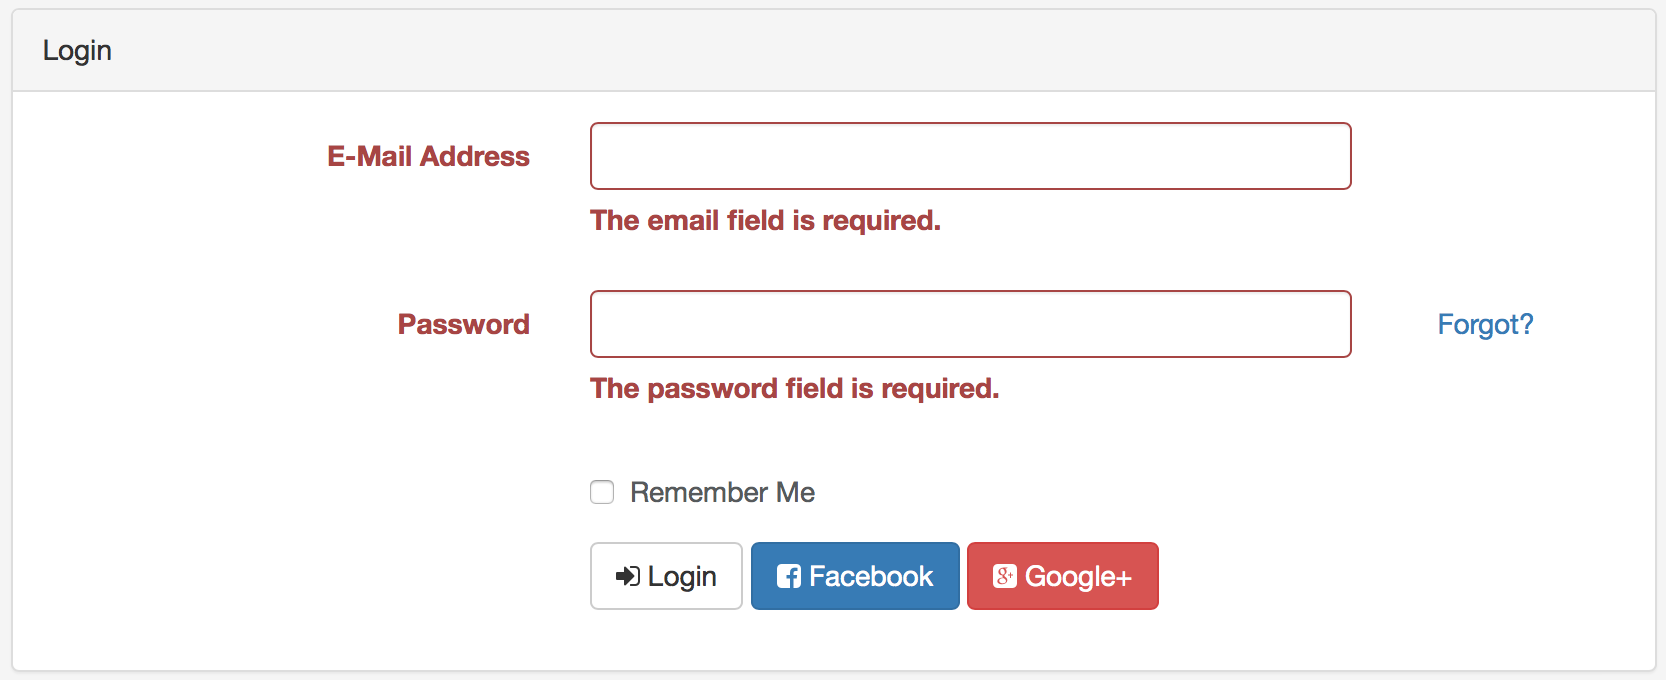
\includegraphics[width=1.0\textwidth]{images/Frisk/Login_Form_Errors}
	\caption{Login Page with Input Errors} \label{fig:Login_Form_Errors}
\end{figure}

\subsubsection{Recover Account}
The reset password page allows the user to recover their account in the case of a forgotten password. The primary purpose of the page is to recover account that were registered manually with an email and password but accounts created using third-party services can also be recovered. The page has a single input for the email address used to create the account and this field is required (see figure \ref{fig:Recover_Form}. Once the user inputs the email and submits the form, the password controller verifies to see if the email is valid. Upon successful validation, the system then generates a recovery code, which is inserted into the password resets table and, emails the user a link to reset their password.

\begin{figure}[H]
	\centering
	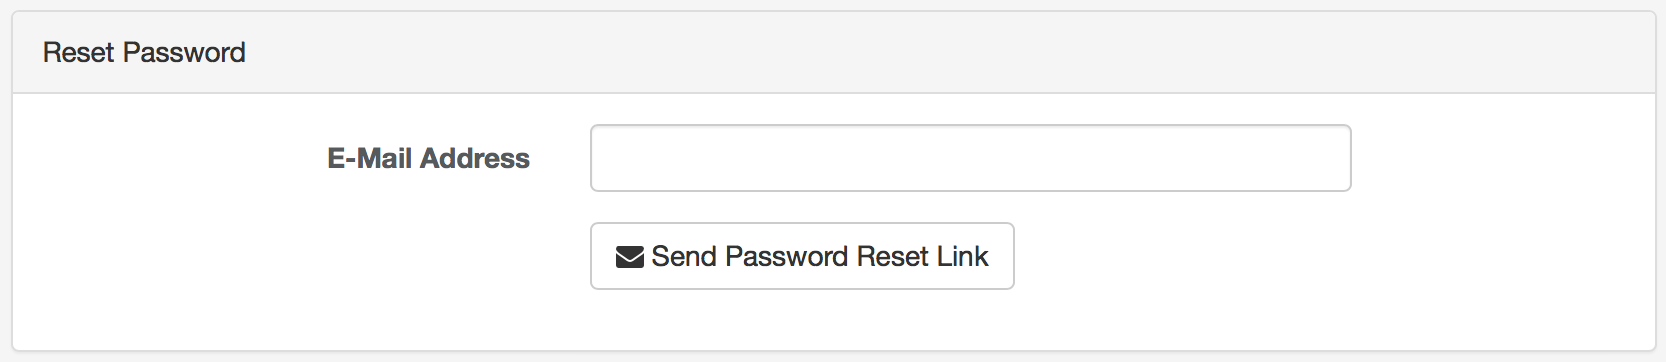
\includegraphics[width=1.0\textwidth]{images/Frisk/Recover_Form}
	\caption{Recover Account Page - Requesting Email} \label{fig:Recover_Form}
\end{figure}

This method can also be used to set a password for accounts created using third-party services as such accounts do not have a password by default. Using the recover link, the user can reset their password by entering their email and a new password. The reset token is valid for one time use only and once the password has been reset, the token is discarded. The password reset form is shown in figure \ref{fig:Reset_Form}.

\begin{figure}[H]
	\centering
	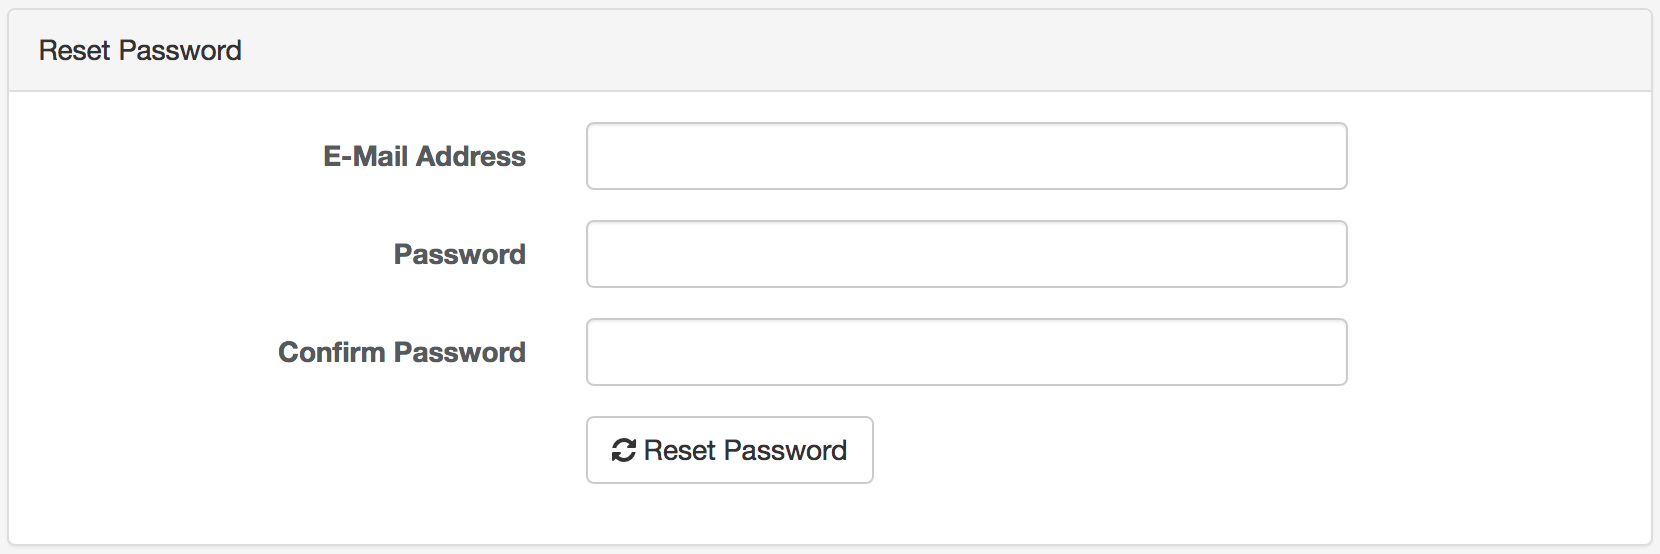
\includegraphics[width=1.0\textwidth]{images/Frisk/Reset_Form}
	\caption{Password Reset Form for Recovering an Account} \label{fig:Reset_Form}
\end{figure}

All the pages covered in this section utilise the guest middleware which ensures that the user can only access this page if they are not already logged in. The only exception to this rule is the logout route which is simply a call to a logout function.

\subsubsection{Authorised Access}

\begin{figure}[H]
	\centering
	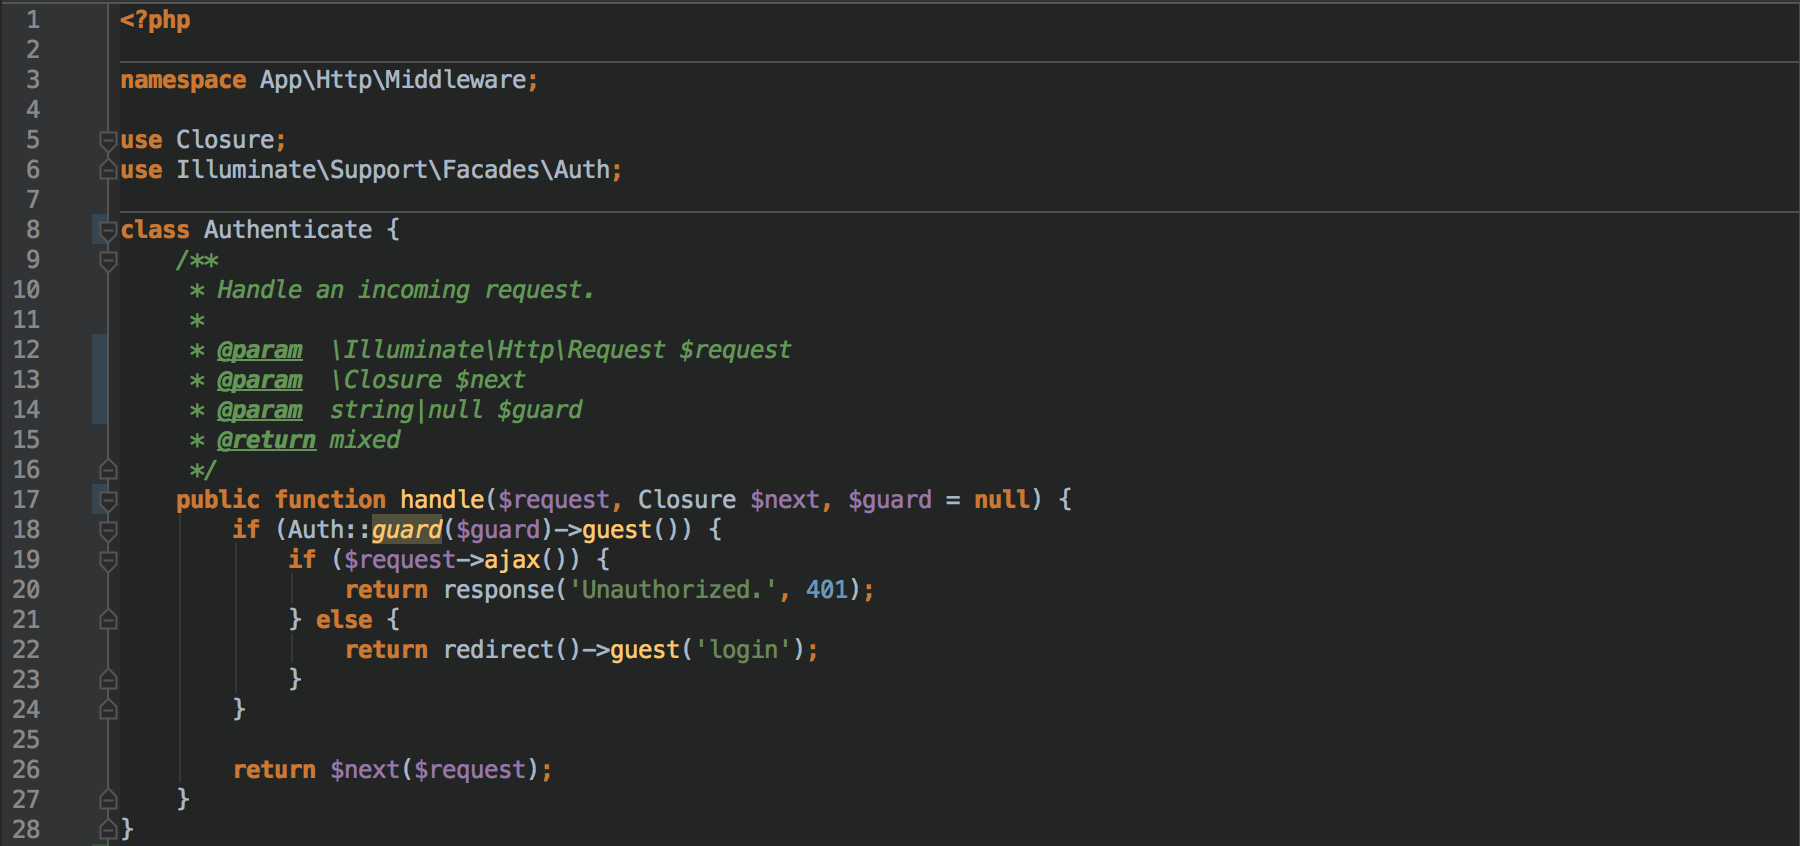
\includegraphics[width=1.0\textwidth]{images/Code/Middleware_Auth}
	\caption{Authentication Middleware for Verifying Users} \label{fig:Middleware_Auth}
\end{figure}

The image in figure \ref{fig:Middleware_Auth} shows the middleware that verifies the user of the application is authenticated. If the user is not authenticated, the middleware will redirect the user to the login screen. However, if the user is authenticated, the middleware will allow the request to proceed further into the application \cite{Laravel:Middleware}. The middleware works by checking if a session exists and a corresponding user can be found in the database. If a user is not found then the user is redirected to the login page for normal requests in contract to AJAX requests, where a 401 error is returned. A middleware providing the inverse operation called \emph{RedirectIfAuthenticated} is also implemented and used on pages such as login and register. This middleware simply redirects the user to the homepage if they are logged and try access a guest only page. 

\subsection{User Interface}
The user interface, being one of the most important parts of the system, must be designed with great care. This means that consistency should be ensured across all pages, be it with the navigation or the general layout. The Laravel blade engine which allows for content to be split across views used to ensure this consistency. This section discusses the tools behind the implementation and how these tools were utilised in the implementation of the user interface rather than the actual functionality provided by the user interface. The functionality is discussed in later sections of the implementation stage.

\subsubsection{Views}
"Views contain the HTML served by your application and separate your controller / application logic from your presentation logic" \cite{Laravel:Views}. The use of views allows content of a single page to be split across multiple files. This can be achieved by abstracting common functionality into separate views that can then be included using \emph{view} global function. A view is usually returned by the closure assigned to a route as following.

\begin{lstlisting}[language=php]
	Route::get('/', function () {
		return view('greeting', ['name' => 'James']);
	});
\end{lstlisting}

As visible in the example above, the \emph{view} function takes a second parameter of type associative array. This can be used to pass variables to the view. Inside the view, you can access each value using its corresponding key, such as \emph{echo \$key}. In the above example, the key name is associated with value James, the user can access the name as a PHP variable \emph{\$name}.

\subsubsection{Blade Templates}
Blade is a powerful templating engine shipped with the Laravel framework. Unlike other frameworks such as Rails, Blade does not restrict the developer from writing plain PHP code inside views. All Blade views end with \emph{blade.php} rather than just \emph{.php}. This allows the views to be compiled into raw PHP code and cached until any further changes are made which means there is essentially no overhead \cite{Laravel:Blade}. In addition to this, Blade also provides shorter syntax for many common tasks such as echoing to the page, loops and conditional statements.


\paragraph{Template Inheritance}
The primary benefits of using the Blade engine over raw PHP files are template inheritance and sections. This allows common code for the outer layout to be abstracted into a single Blade view which will be used as the master view. The purpose of this functionality is to allow the developer to provide consistency across pages and reduce the amount of duplicate code. For example, the navigation will be consistent across all pages and hence this can be abstracted into the master view and if changes need to be made to the navigation then updating the master view will update all pages. A view may only extend one other view but the parent may extend another view forming a hierarchy of inheritance. 

\begin{figure}[H]
	\centering
	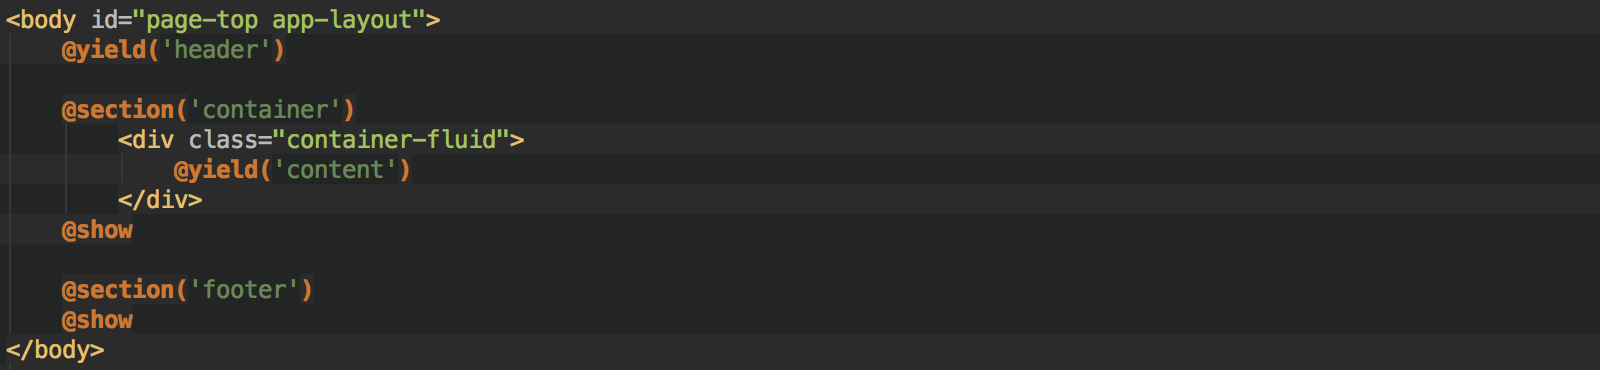
\includegraphics[width=1.0\textwidth]{images/Code/Master_View}
	\caption{Master View - Used by Pages and Dashboard} \label{fig:Master_View}
\end{figure}

Figure \ref{fig:Master_View} shows a part of the code to define the base layout for our application, inherited by the pages template and dashboard template. As you can see, this file contains typical HTML mark-up but also additional syntax, take note of the \emph{@section} and \emph{@yield} directives. The \emph{@section} directive, as the name suggests, defines a section of content in the document, which can be extended or overridden by a child view, whereas the \emph{@yield} directive is like a placeholder displays the content of a section that may optionally be define in a child view.

\begin{figure}[H]
	\centering
	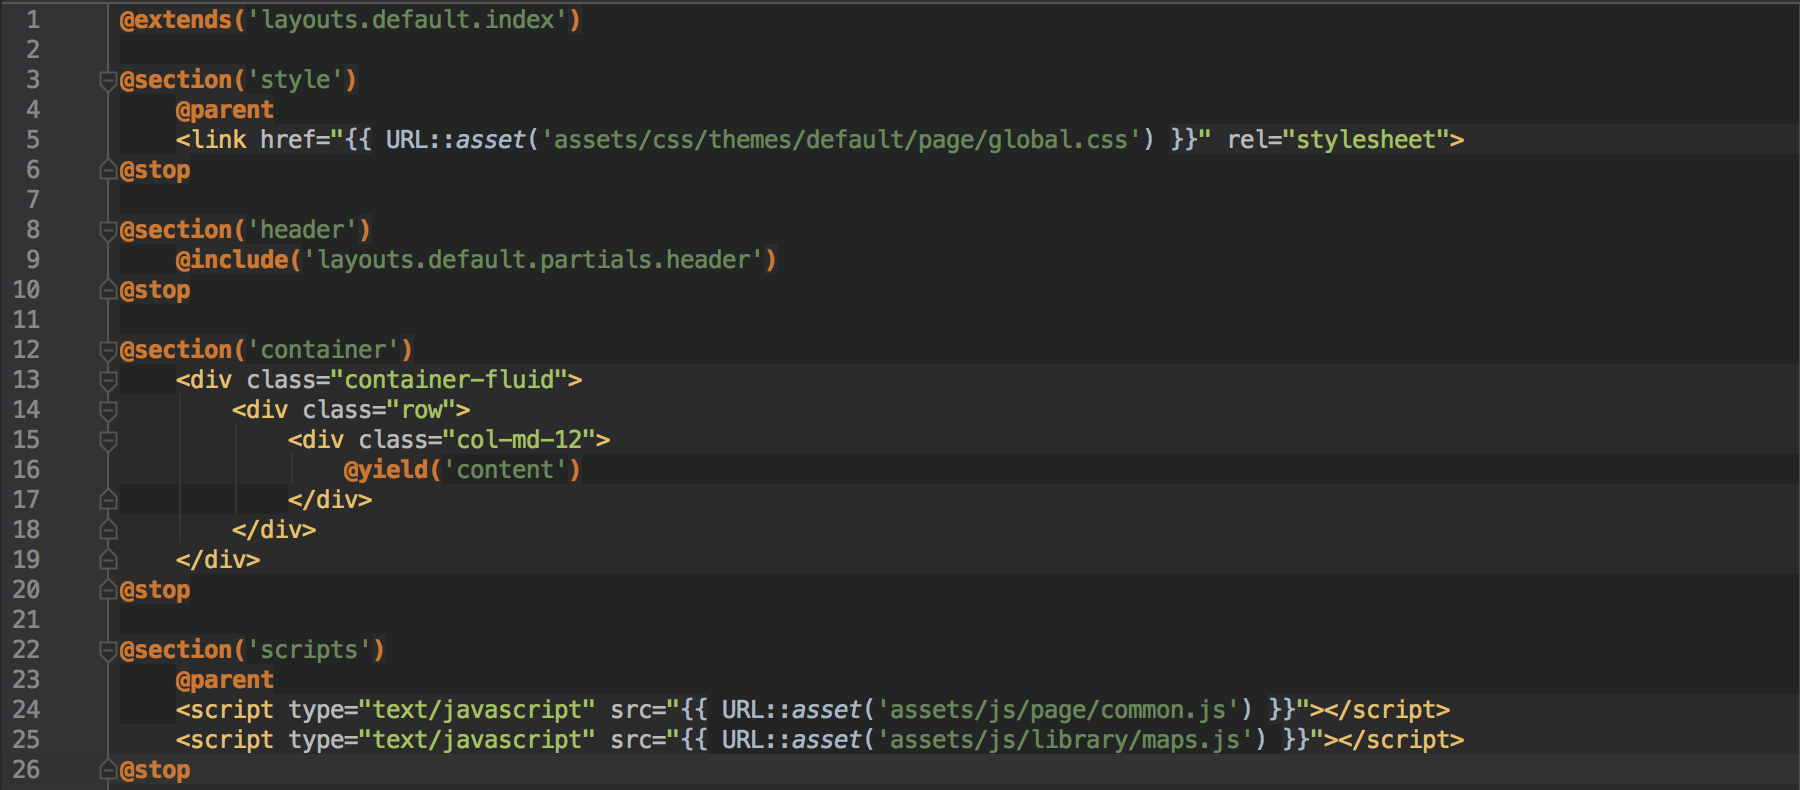
\includegraphics[width=1.0\textwidth]{images/Code/Master_Page}
	\caption{Master View for Pages - Inherits Base Master View} \label{fig:Master_Page}
\end{figure}

When defining a child view or page, as shown in figure \ref{fig:Master_Page}, the Blade @extends directive can be used to specify which layout the child page should "inherit" \cite{Laravel:Blade}. Views which extends a master view can inject content into the master view using the \emph{@section} directive as long as the parent has \emph{@yield} directive for the section. In the example, the secondary master layout for pages extends the primary base layout and overrides the parents container with custom content but then allows extending views to define the content within the container. The \emph{@include} directive is used to include a partial view containing the page header which consists of the navigation and any page headings. The example is utilising the @parent directive to append (rather than overwriting) content to the layout's style and scripts section. "The @parent directive will be replaced by the content of the layout when the view is rendered" \cite{Laravel:Blade}.

\subsection{Pages}
As mentioned in the design section, the pages represent the collection of webpages on the public front end that are available to all users, authenticated or not. The design for the pages consists of a master layout which is inherited from a base layout. This master layout can then be extended by all pages and the content can be implemented individually.

\subsubsection{Commonalities}
In order to provide familiarity to user, there are common features throughout the system. These include things such as the site-wide layout, navigation, footer and additional code for performance.

\paragraph{Layout}
The theme for all the pages was inspired by the design of a popular hotel rental company, AirBNB\cite{AirBnB:Home}. The layout and the design were developed from new without the use of any existing templates or code from any third-parties. The icons used throughout the system are provided by the FontAwesome repository as well as the Glyphicon font provided by Bootstrap. A consistent font is used throughout the entire theme across all pages but varying font sizes and colours have been employed. This combination of services and tools provides a sleek and professional finish.

The layout contains the navigation bar at the top of the page which is discussed further below. In addition to this, the layout provides a container as well as any scripts and stylesheets for the design in the master view. The child pages will simply implement the content of the container. The container provides a margin on both sides as well as the top to distance the content from the edges and the navigation in order to increase readability.

\paragraph{Navigation}

\begin{figure}[H]
	\centering
	\begin{subfigure}[t]{1\textwidth}
		\centering
		
\includegraphics[width=1.0\textwidth]{images/Frisk/Nav_Default}
		\caption{Navigation Bar for Guest Users}\label{fig:Nav_Default}		
	\end{subfigure}
	\quad
	\begin{subfigure}[t]{1\textwidth}
		\centering
		
\includegraphics[width=1.0\textwidth]{images/Frisk/Nav_Authenticated}
		\caption{Navigation Bar for Authenticated Users}\label{fig:Nav_Authenticated}
	\end{subfigure}
	\caption{Navigation Bar for Pages (Guest VS Authenticated}\label{fig:AuthVSDefaultNav}
\end{figure}

Without the navigation the user would be unable to browse the system. The same applies if the navigation headings are unintuitive as users would have to browse through all the links to find the page they need. For this reason, the navigation was kept extremely simple with only the most necessary links. A different set of links is presented to the user depending on whether they are authenticated or not. In both cases the logo, is presented to the user which redirects the user to the homepage, along with the search bar to provide easy searching without having to come back to the homepage.

Figure \ref{fig:Nav_Default} shows the navigation bar presented to the user if they are a guest, containing just three links for explore, login and register. Figure \ref{fig:Nav_Authenticated} shows the alternate navigation bar, presented to user once they've authenticated by signing into the system. This time the navigation bar contains the link for explore, messages and a dropdown menu with the users name. This dropdown provides further links, one for the dashboard and another for logging out.


\subsubsection{Home}
The homepage contains all the basic features that are inherited from the templates. The main feature of note on the homepage is the crime map which is generated using the police data API and is updated live as soon as new data becomes available on the public database. This is shown in figure \ref{fig:Home_Map}. As the crime map spans the full width of the page, where as the container leave a margin on both sides, this meant the container section from the master layout had to be overridden to provide this different functionality.

\begin{figure}[H]
	\centering
	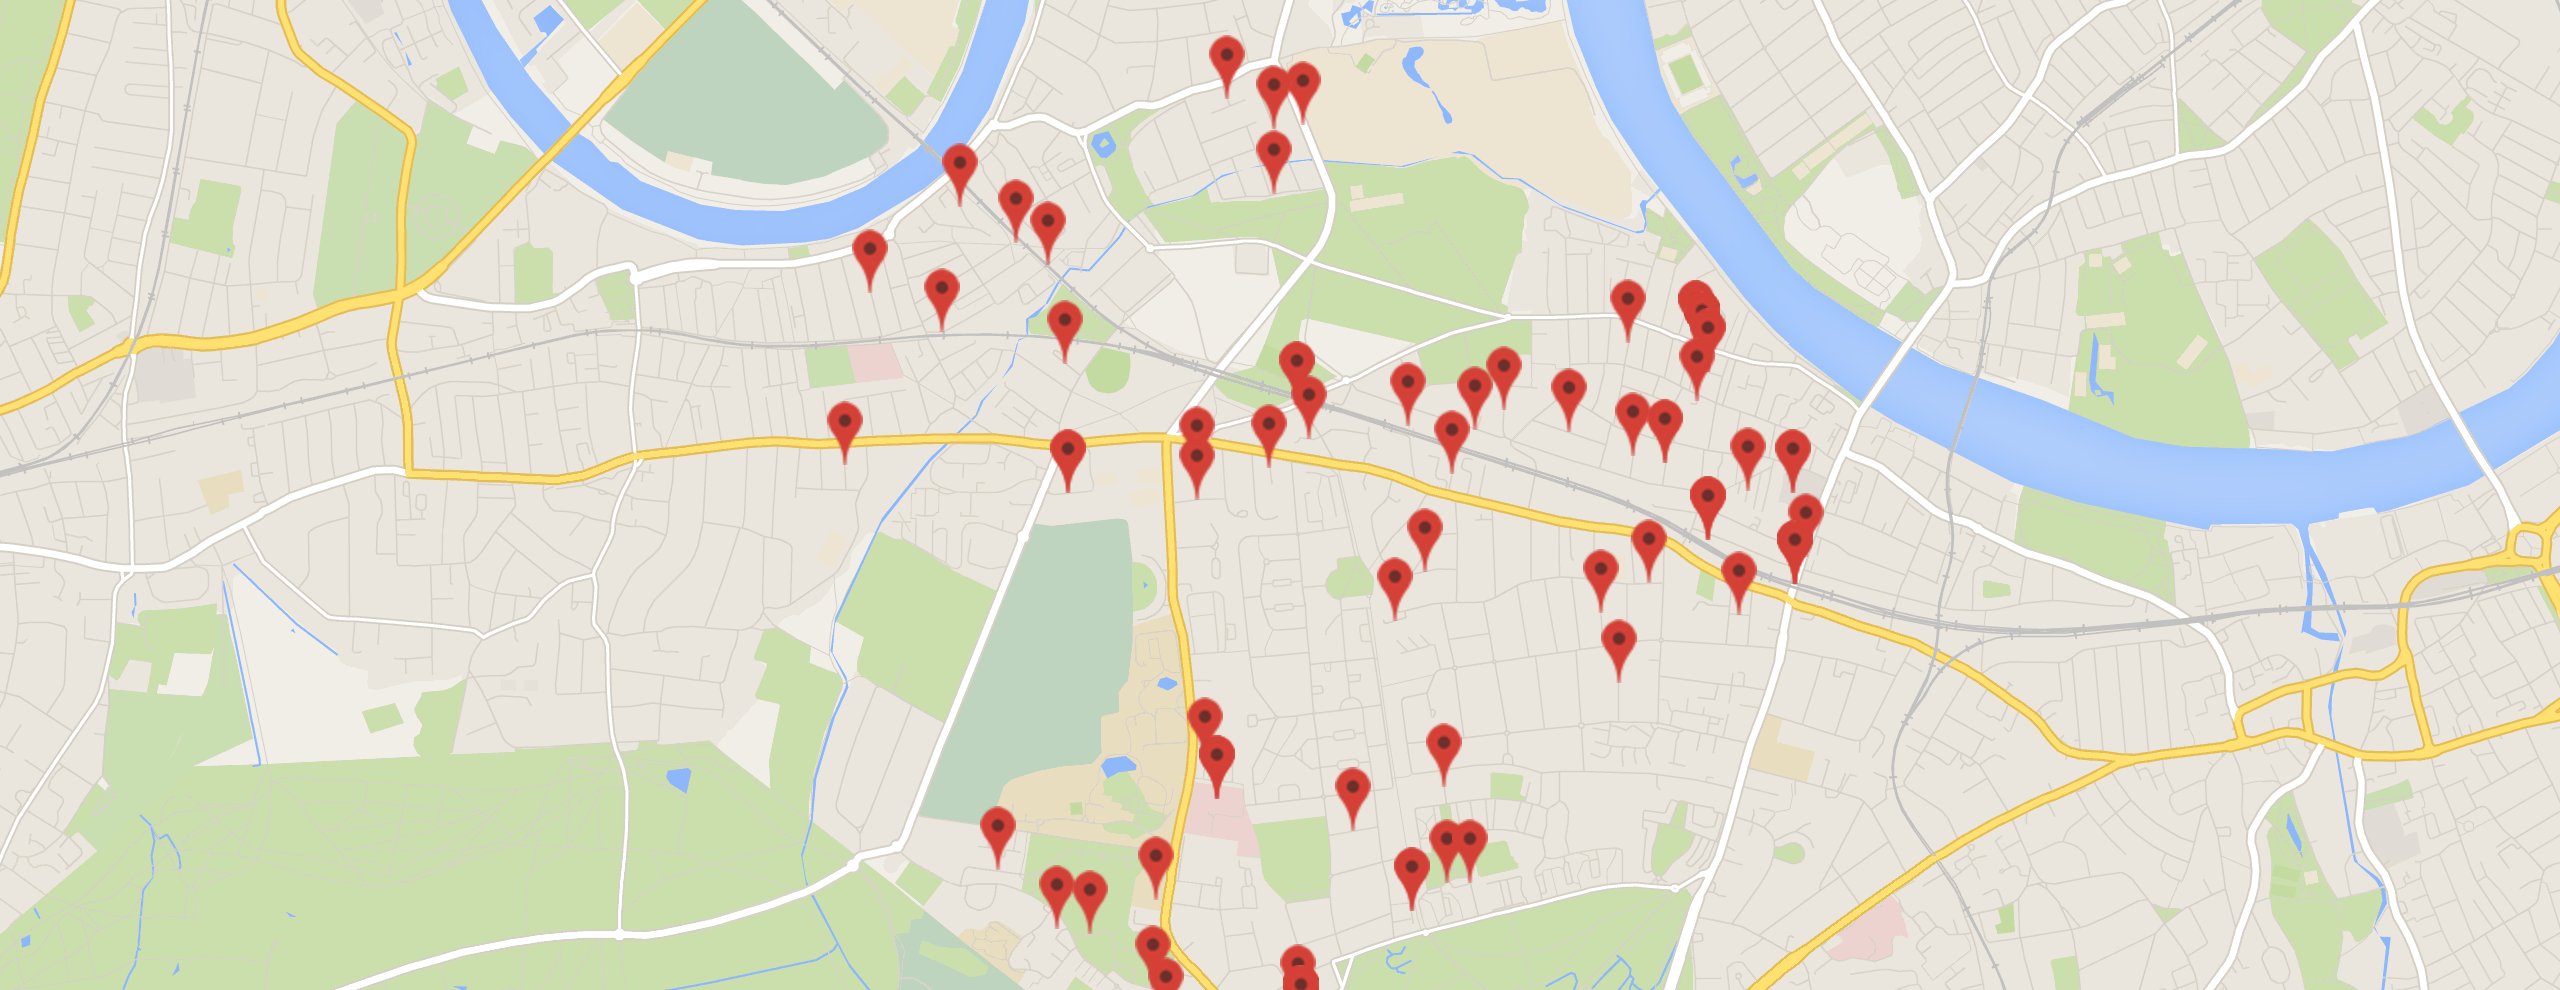
\includegraphics[width=1.0\textwidth]{images/Frisk/Home_Map}
	\caption{Live Crime Map on the Homepage} \label{fig:Home_Map}
\end{figure}

In order to generate the crime the Google maps JavaScript API was used along with the police data API. The first step requires the users current location which is retrieved using the geolocation services provided in HTML 5. Once the users location is retrieved, an AJAX call is made to the police API, with the coordinates as a parameter, which returns the results of the query as a JSON output. This is captured in the data variable of the JSON callback function. Once the results have been retrieved, JavaScript is used to loop through the collection and filter any results from the burglary, theft and robbery category. These filtered results are added to the map using markers, also provided by the Google Maps API. The \emph{addMarker} method shown in the figure was created as part of a wrapper which simplifies the creation and management of maps created using the Google Maps API.

\begin{figure}[H]
	\centering
	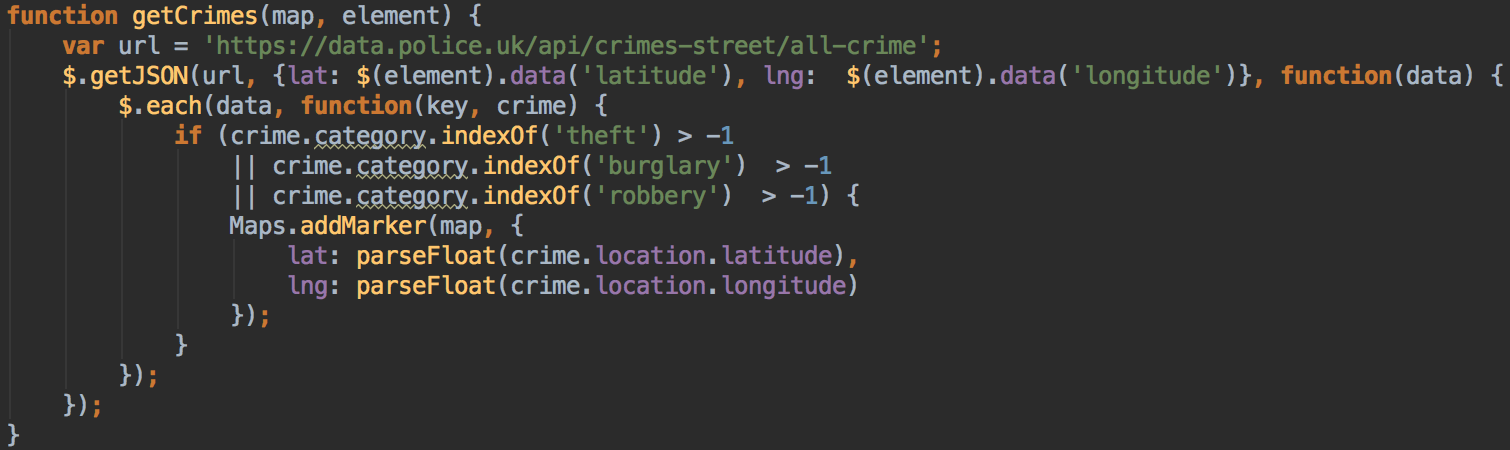
\includegraphics[width=1.0\textwidth]{images/Code/Home_Map}
	\caption{Code for Generating the Live Crime Map on the Homepage} \label{fig:Home_Map_Code}
\end{figure}

\subsubsection{Search}
The search page allows the user to search for items using either the name or the unique identifier. The design of the page is pretty similar to the rest of the pages where the standard navigation bar is included at the top. The search results are then displayed as tiles using bootstrap columns. A four column layout is used which means, on the desktop version of the site, up to 4 results can show up in a single row but the number is lower on mobile devices.

\begin{figure}[H]
	\centering
	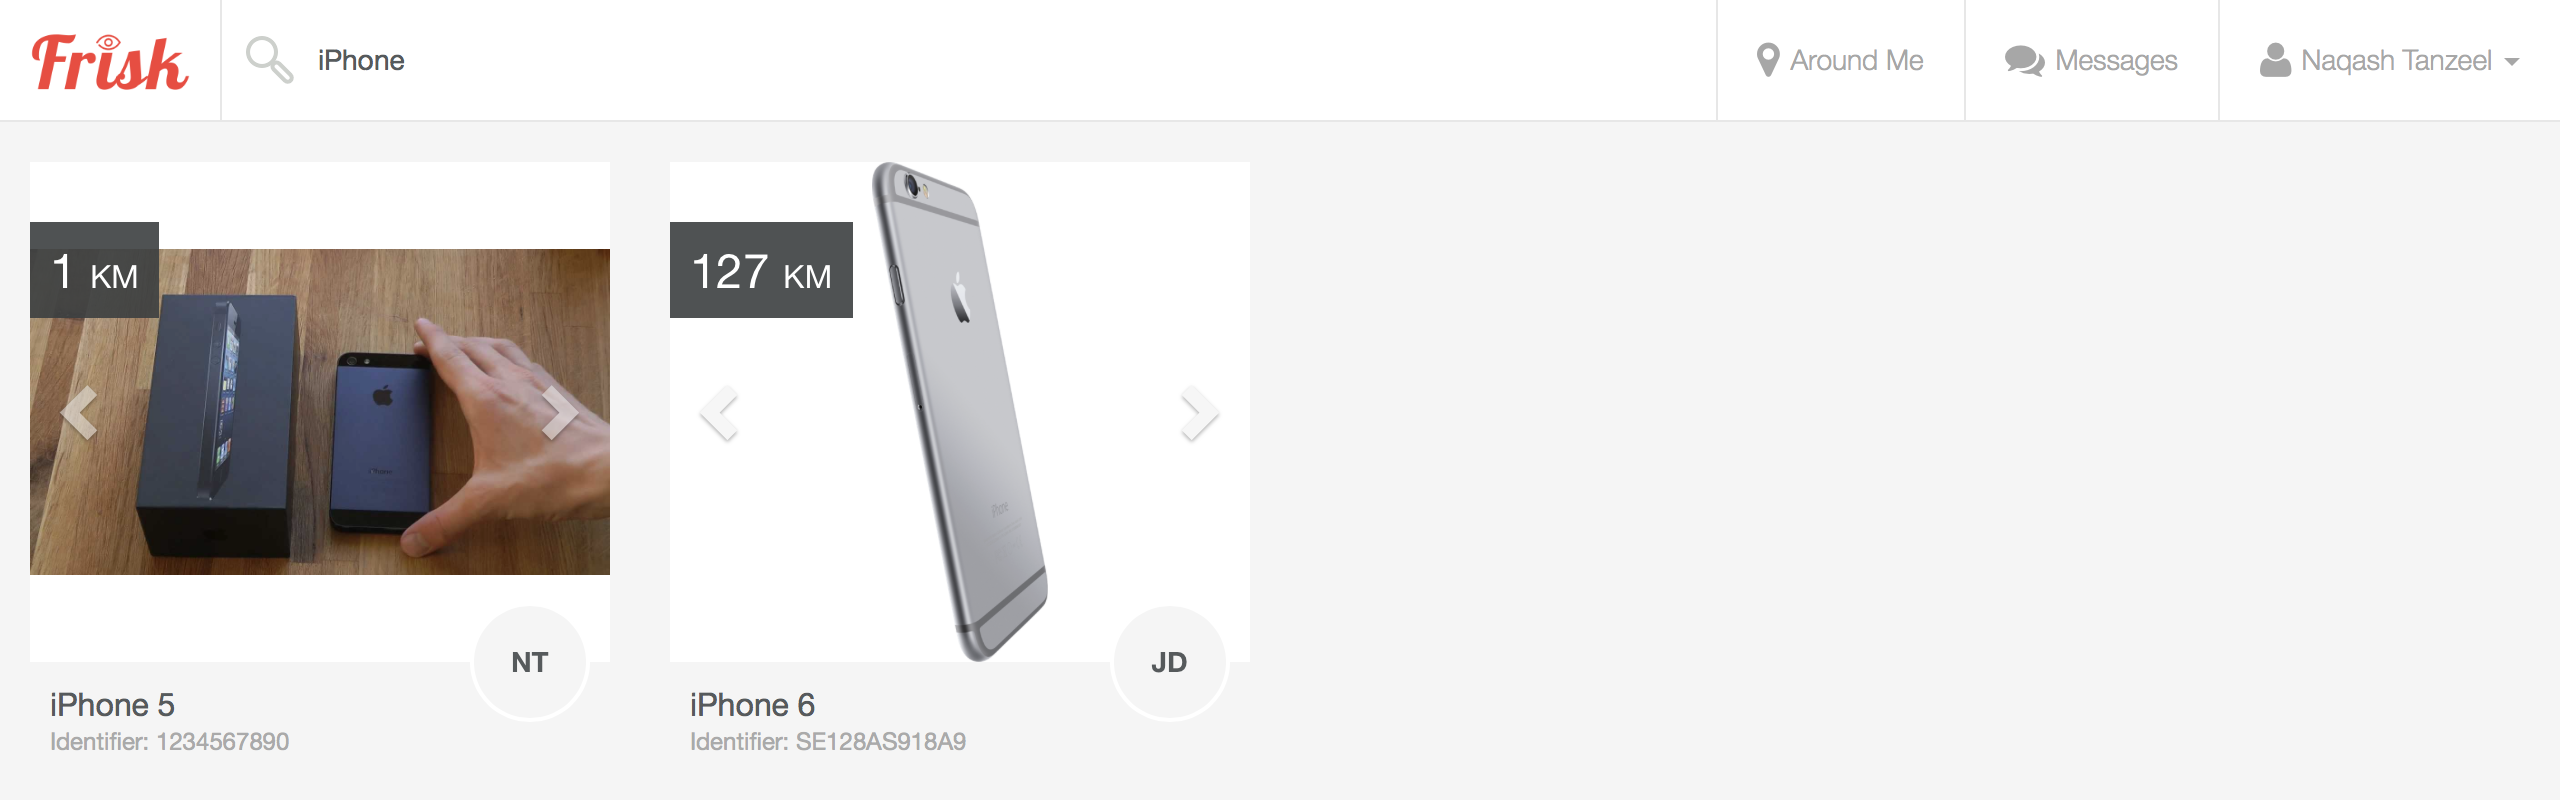
\includegraphics[width=1.0\textwidth]{images/Frisk/Search_Results}
	\caption{Search Results on the Search Page for 'iPhone'} \label{fig:Search_Results}
\end{figure}

As visible in the figure \ref{fig:Search_Results}, the results include several details about the time. Firstly, an image is displayed for the item which is the cover image for the item. The user can scroll through all the public images of the item without having to open the view item page. This functionality is implemented using the default carousel built into the Bootstrap package. The design of the carousel was altered slightly to remove unnecessary shadows and gradients and provider a simpler experience. The name, and unique identifier of the item is also listed so the user can quickly identify whether this is the result they were looking for and if not, skip to the next one. The owners initials have also been included in the result for security reasons so that the users can be vaguely identified, in the case of spammers.

\begin{figure}[H]
	\centering
	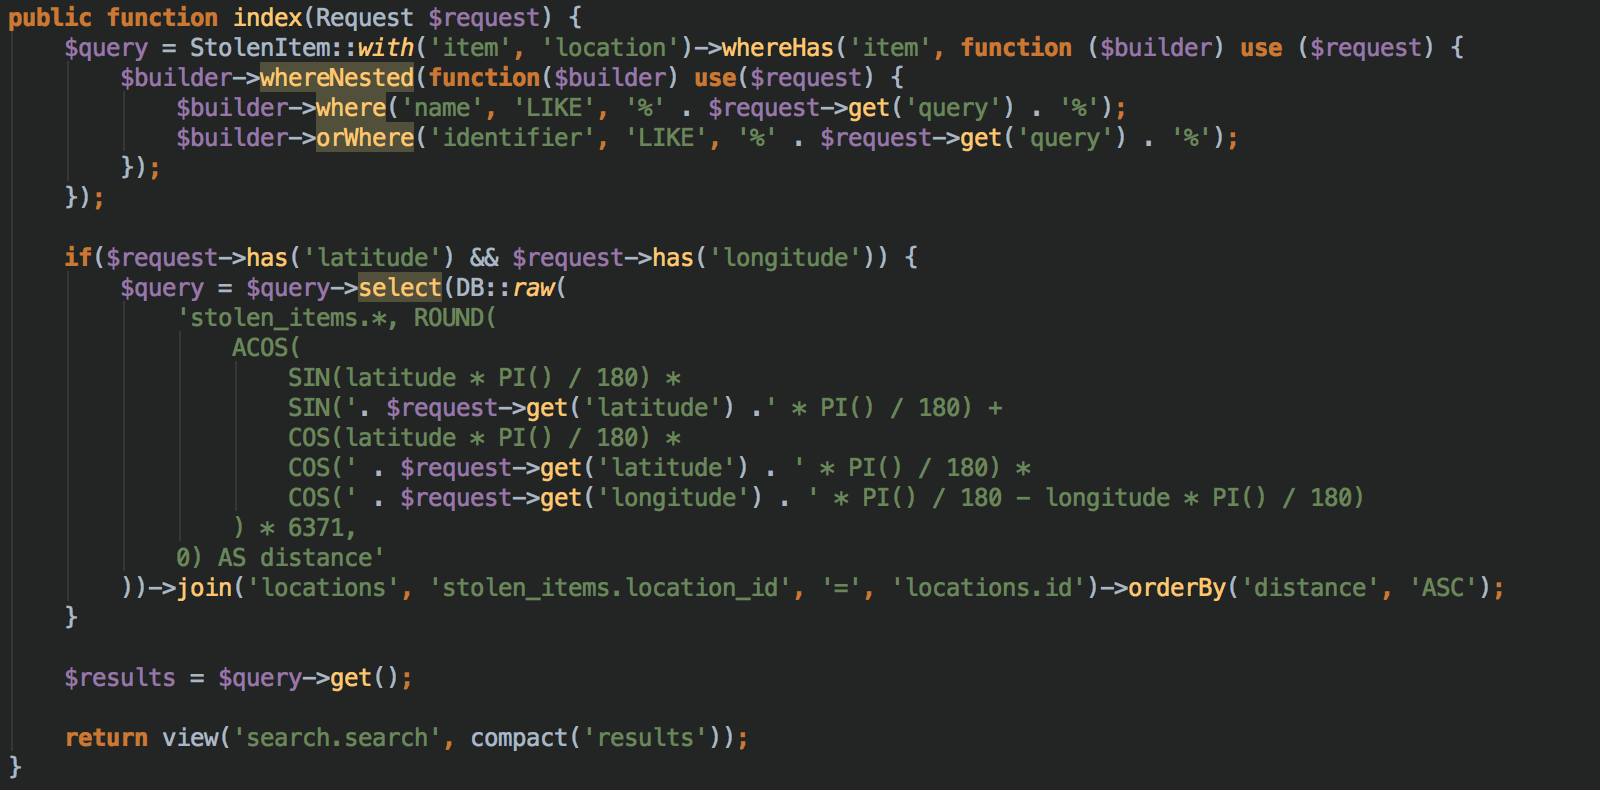
\includegraphics[width=1.0\textwidth]{images/Code/Search}
	\caption{Search Feature Algorithm and Queries} \label{fig:Search_Code}
\end{figure}

The user could optionally provide their current location to enhance the search feature, which would list the distance from their current location for each item returned as a result for their query. Figure \ref{fig:Search_Code} shows the method that is called when the user visits the search page and the code used to generate the results. 

The code in the image works by finding all the stolen item records which are then along with their corresponding location of theft. Additionally the item corresponding to the theft record is also retrieved, allowing the query to filter only stolen items which have a corresponding item that matches the search query. The items are filtered by either the name or identifier, either match will result in the item being returned. The next part checks to see if the request has a latitude and longitude in the url. If both components of a coordinates are found in the URL then a raw query is added to compute the distance from the theft location. In order to achieve this, the locations table must be joined onto the results. The distance between coordinates is computed using the Haversine formula, discussed further in the explore section. Finally the results are ordered by distance and fetched by calling the \emph{get} method on the query builder. The search results view is returned by the closure which will display the results to the user.

\subsubsection{Explore}
\begin{figure}[H]
	\centering
	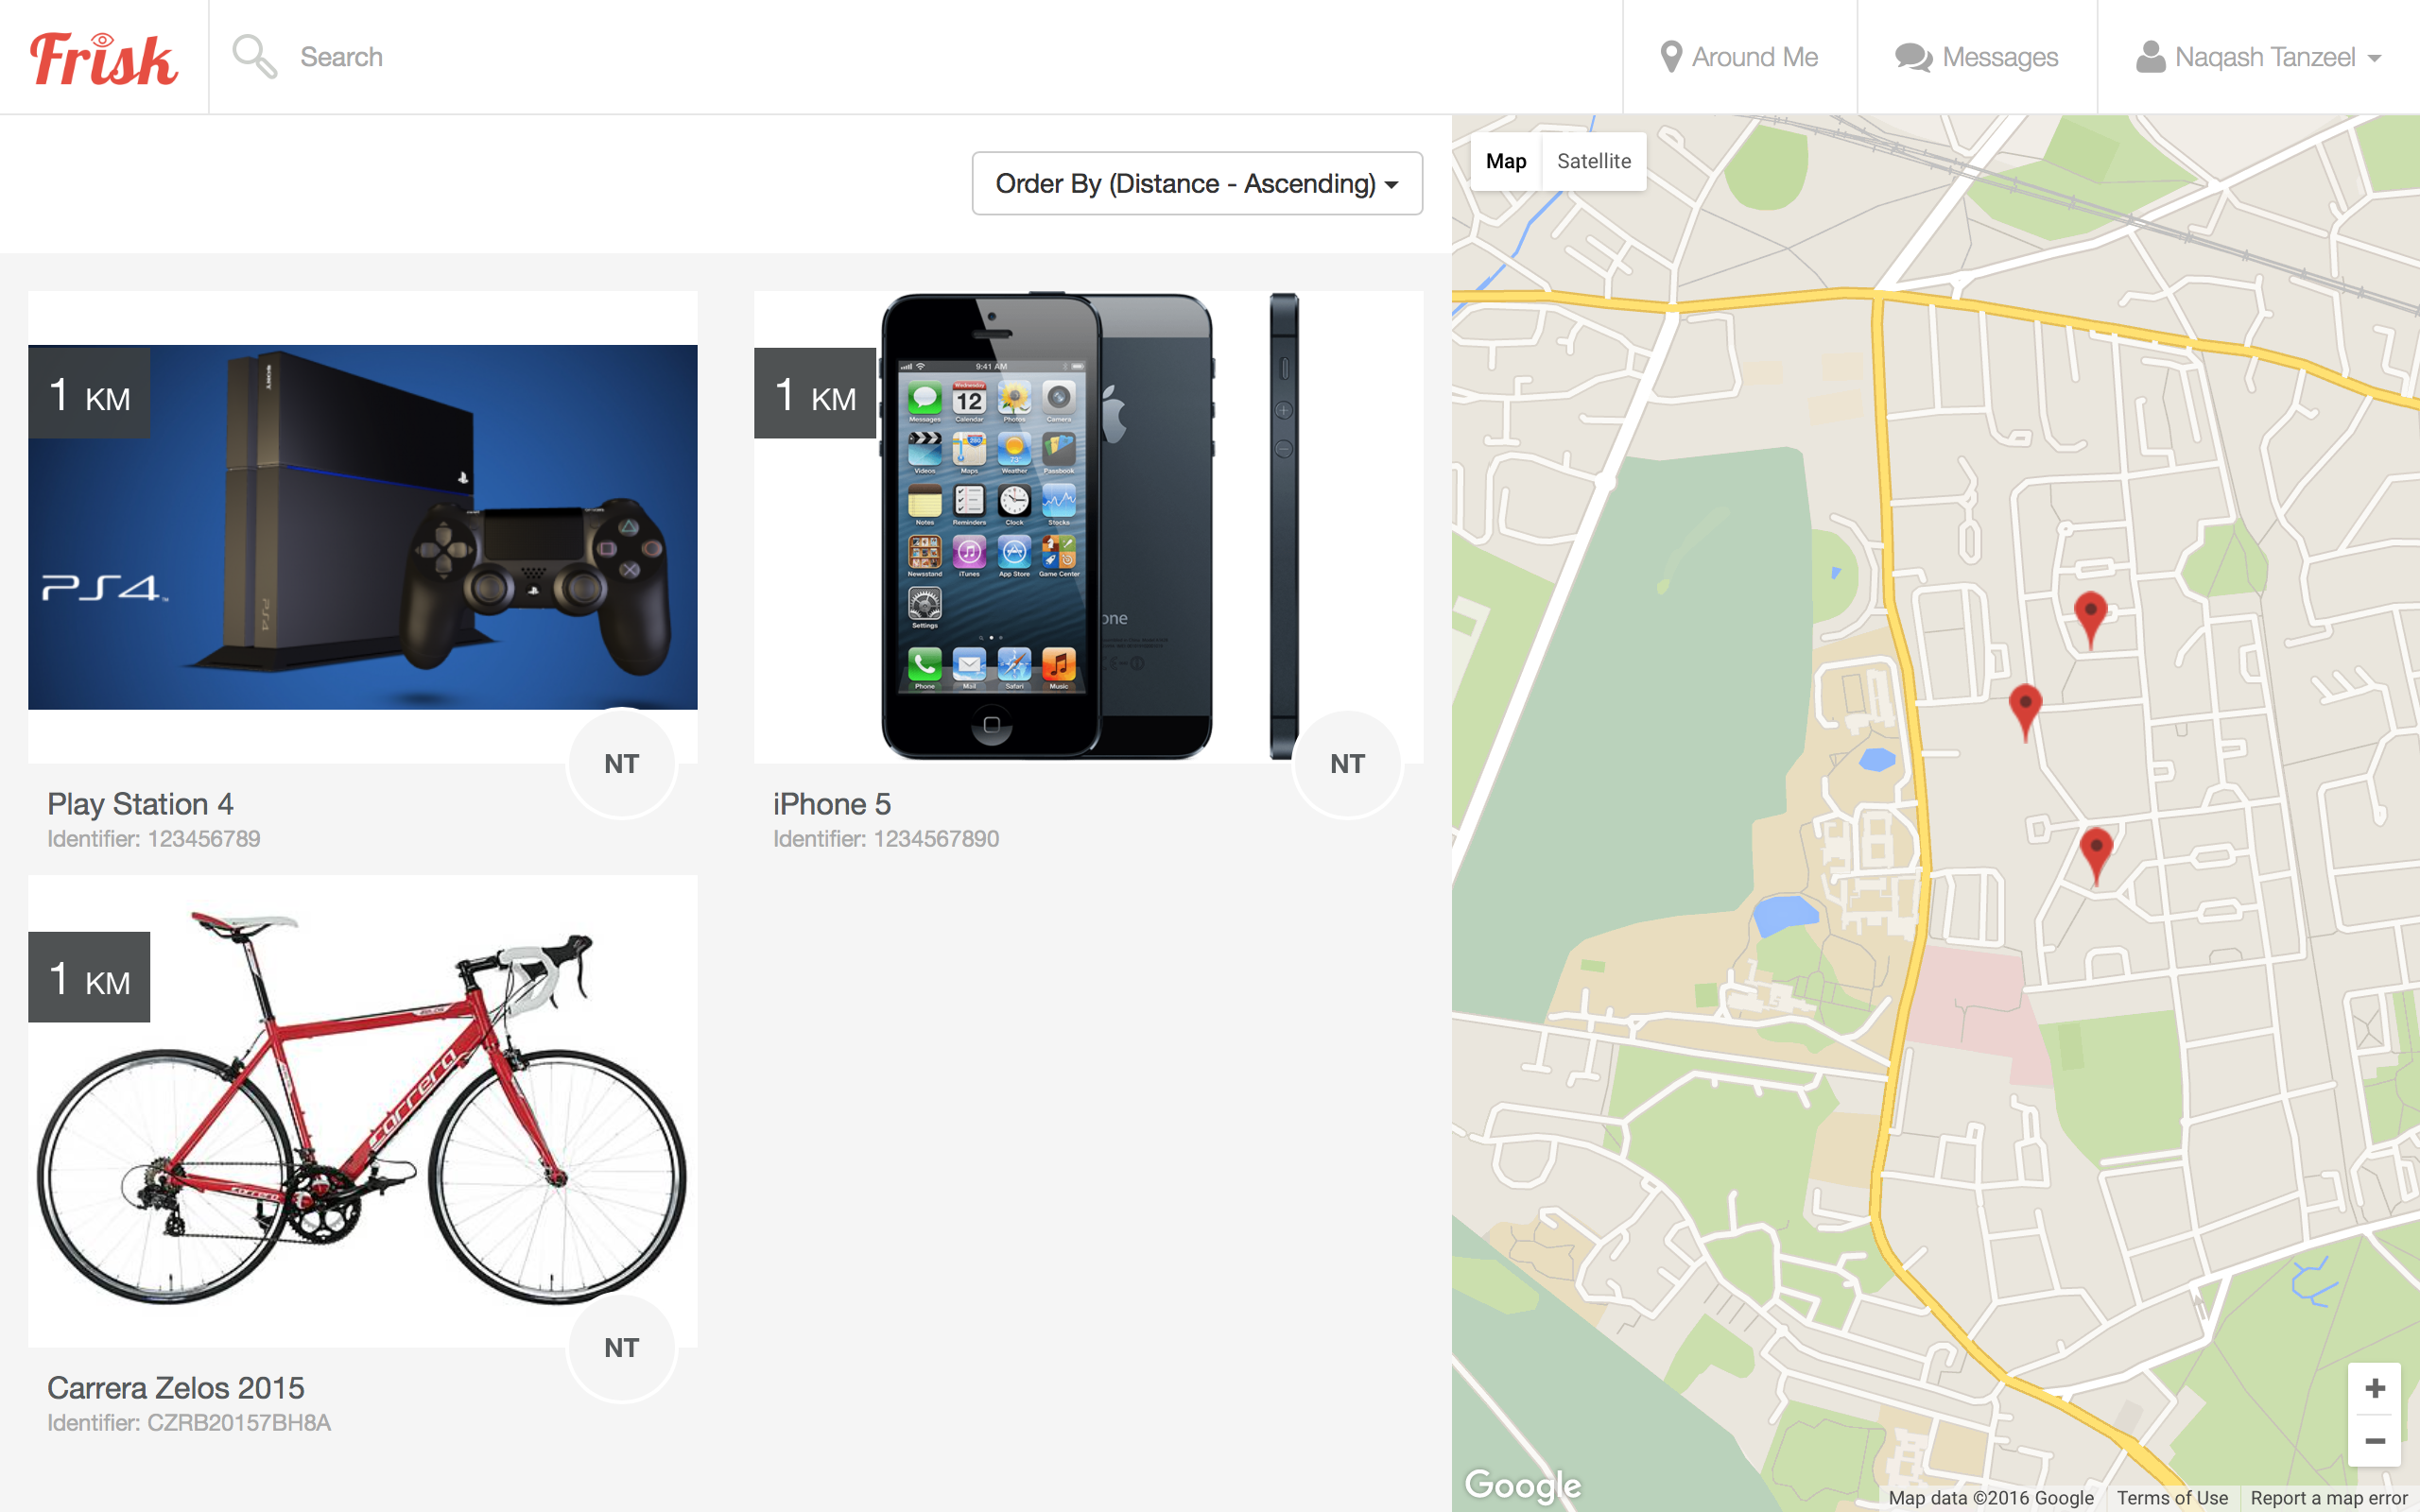
\includegraphics[width=1.0\textwidth]{images/Frisk/Around_SW15}
	\caption{Explore Page for Area with Postcode SW15} \label{fig:Around_SW15}
\end{figure}

The explore allows the user to explore reports of theft and burglaries in their local area. This page is only accessible if the user allows the system to use their current location as this is required to find items within their local area. The page once again contains the basic layout from the template but, unlike other pages, it overrides the default container and implements a custom wrapper. This is because the functionality of the page is split into two sections. 60\% of the page on the left hand side provides results in a grid, similar to that of the search page whereas the remaining 40\% on the right hand side is used for an interactive map. Unlike the search page, the user is able to sort the results in the grid view by either name or distance as both are guaranteed to be available on this page.

\paragraph{Passing Map Data From PHP to JavaScript}

In order to generate the map the coordinates for the centre are assigned to attributes of the element that will contain the map. Upon page load, JavaScript is used to loop through all elements with the \emph{.map} class and these attributes are read, making it simple to transfer data retrieved by PHP to scripts written in JS. This allows a map with a specific centre to be generated. However, as the data for the markers is also retrieved through PHP, this still leaves the problem of passing this data to the JS scripts. In order to combat this problem, a custom class was written which acted as a global dictionary and retained information until the page was reloaded. The array containing the markers data is converted to JSON format and assigned to a key in this dictionary before the script for generating the markers is loaded. Once the script loads, it can read the data from the dictionary and generate the map.

\begin{figure}[H]
	\centering
	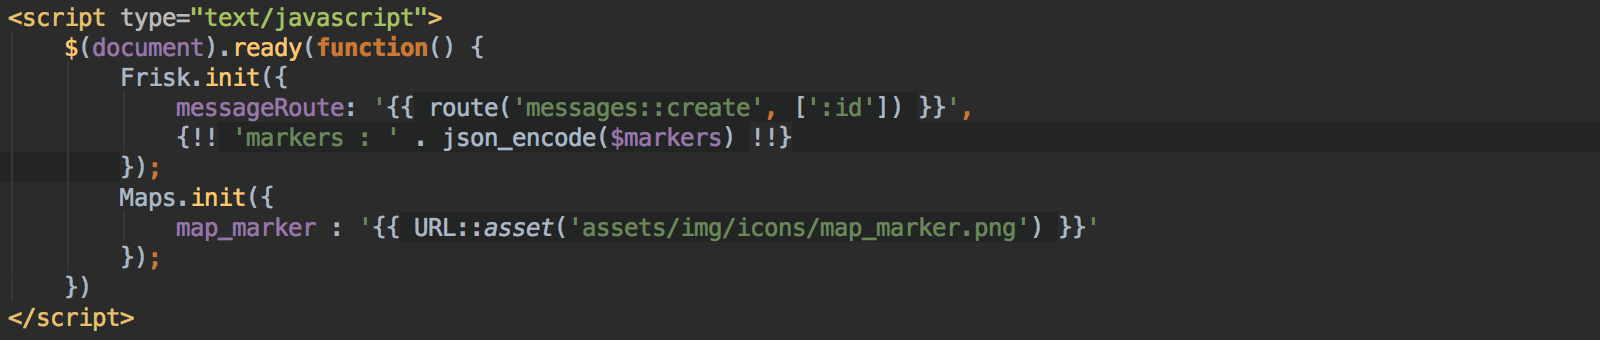
\includegraphics[width=1.0\textwidth]{images/Code/Locations_PHP_To_JS}
	\caption{Passing an Array of Data from PHP to JavaScript} \label{fig:Locations_PHP_To_JS}
\end{figure}

\paragraph{Haversine Formula}
The distance computation on both the search and the explore page uses the ‘Haversine’ formula to calculate the great-circle distance between two points – that is, the shortest distance over the earth’s surface – giving an ‘as-the-crow-flies’ distance between the points \cite{MovableType:Haversine}. 

\begin{equation}
	a = sin^2 (\triangle \frac{\phi}{2}) + cos (\phi_1) * cos (\phi_2) * sin^2 (\triangle \frac{\lambda}{2})
\end{equation}
\begin{equation}
	c = 2 * atan^2(\sqrt{a}, \sqrt{1-a})
\end{equation}
\begin{equation}
	distance = R * c
\end{equation}

This formula above can quickly and efficiently compute the distance between two coordinates where $\phi$ is latitude, $\lambda$ is longitude, and R is the earths radius (6371 km). However with the use of the haversine formula variables names are required which overcomplicates the SQL query. Instead a tweaked version of this involving the law of spherical cosines was used to compute the distance to an accuracy of a few meters. This provided a shorter one line alternative to the haversine meaning it was easier to implement using SQL. The code shows an example SQL query that could be used to compute the distance between the users location and a location from the database where \emph{:userLatitude} and \emph{:userLongitude} must be replaced with the current users latitude and longitude respectively.

\begin{lstlisting}[language=sql]
	SELECT ACOS(SIN(latitude * PI() / 180) * SIN(:userLatitude * PI() / 180) + COS(latitude * PI() / 180) * COS(:userLatitude * PI() / 180) * COS(:userLongitude * PI() / 180 - longitude * PI() / 180) ) * 6371000 AS distance FROM locations
\end{lstlisting}

\begin{figure}[H]
	\centering
	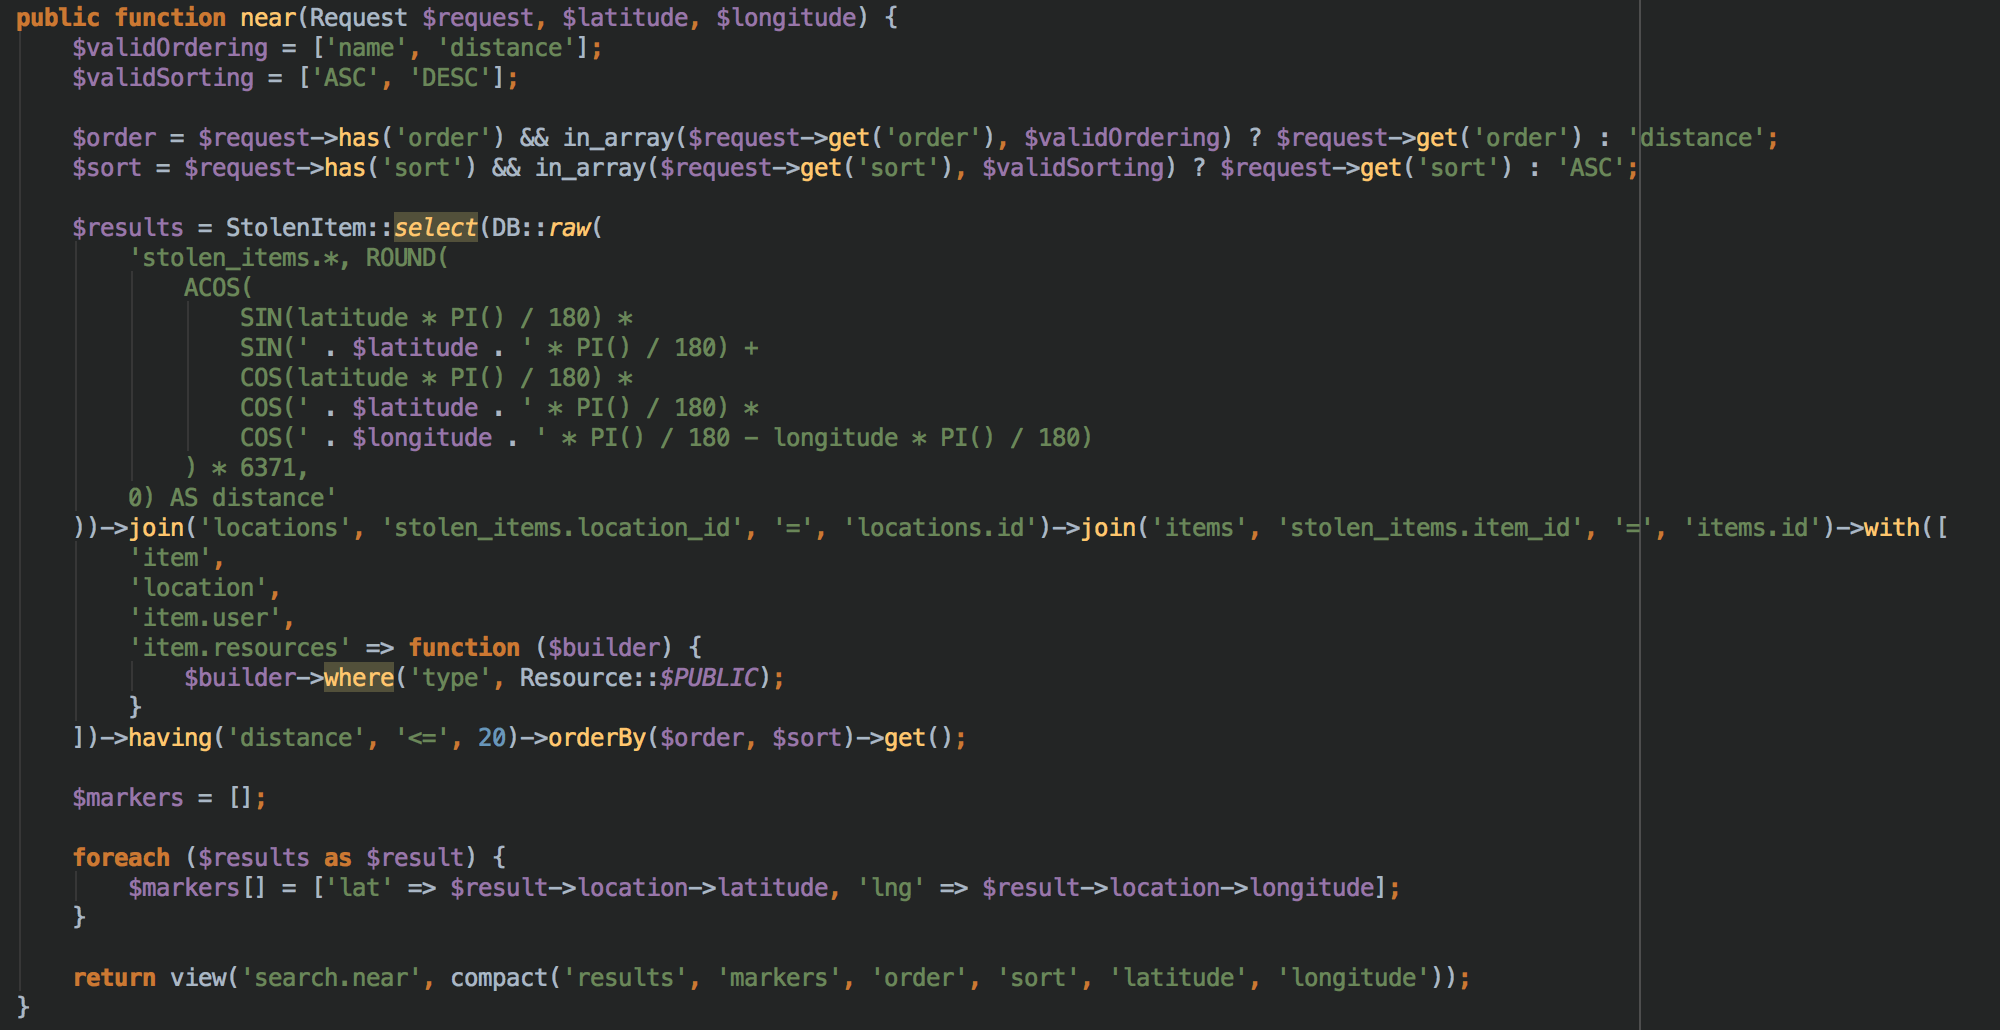
\includegraphics[width=1.0\textwidth]{images/Code/Explore}
	\caption{Explore Feature Algorithm and Queries} \label{fig:Explore_Code}
\end{figure}

Figure \ref{fig:Explore_Code} shows the code that is executed when the user navigated to the explore page. The latitude and longitude are passed to the method as parameters which are captured from the URL automatically by the Laravel framework. If either of these parameters is missing then the method simply won't be called. Once all the prerequisites have been met and the method is called, checks are made to ensure that the ordering attribute and sorting options are valid. If these checks are failed then the system simply resorts to a default ordering. Next the query discussed earlier is used to compute the distance of the item, similar to the search page, and the stolen item records along with the corresponding location, item, user, and resource are fetched. The results are filtered by limiting the distance to 20 KM and finally ordered, based on the users request. This is enough for generating the grip view for the results but an additional step needs to be taken to produce the map. An array of all the markers is generated by looping through each result and collating the coordinates as a dictionary with the keys \emph{lat} and \emph{lng}. The view can now be rendered by passing all this data using the compact method which finds all variables with the specified names and created a dictionary of these. The rendered view is returned to the user and the page finishes loading from the server side but client sided code is executed to generate the map.

\subsubsection{View Item}
The user is able to view more details about an item including the description, postcode and more. This is offered through a Bootstrap modal which already exists on the page to reduce load time whenever the user wants to view an item. The user cab bring up the modal to view the details by clicking the result tile on the search or explore page. The modal is split into two sections where the left contains a bootstrap carousel allowing the user to browser all the public images for the item. This was initially problematic as images were of different sized which caused the entire modal to resize but the problem was overcome by using absolute position and setting the images as a css background rather than a standard image. The second part of the modal contains the name of the items and some further details along with a a link to contact the owner of the item.  The messaging feature is only available to registered and hence if an unauthenticated user clicks the message link they are are redirected to the login page.

The information to populate the modal is loaded through an AJAX call which returns all the details in a JSON format. Initially a HTML view was returned but this was later switched to JSON as this increased the response due to less content being transferred over the network. The JSON details are then used to populate the modal and present it to the user. The design of the modal changes on mobile view such that the title is followed by the images and then the details are displayed below the images to provide an easier experience.

\begin{figure}[H]
	\centering
	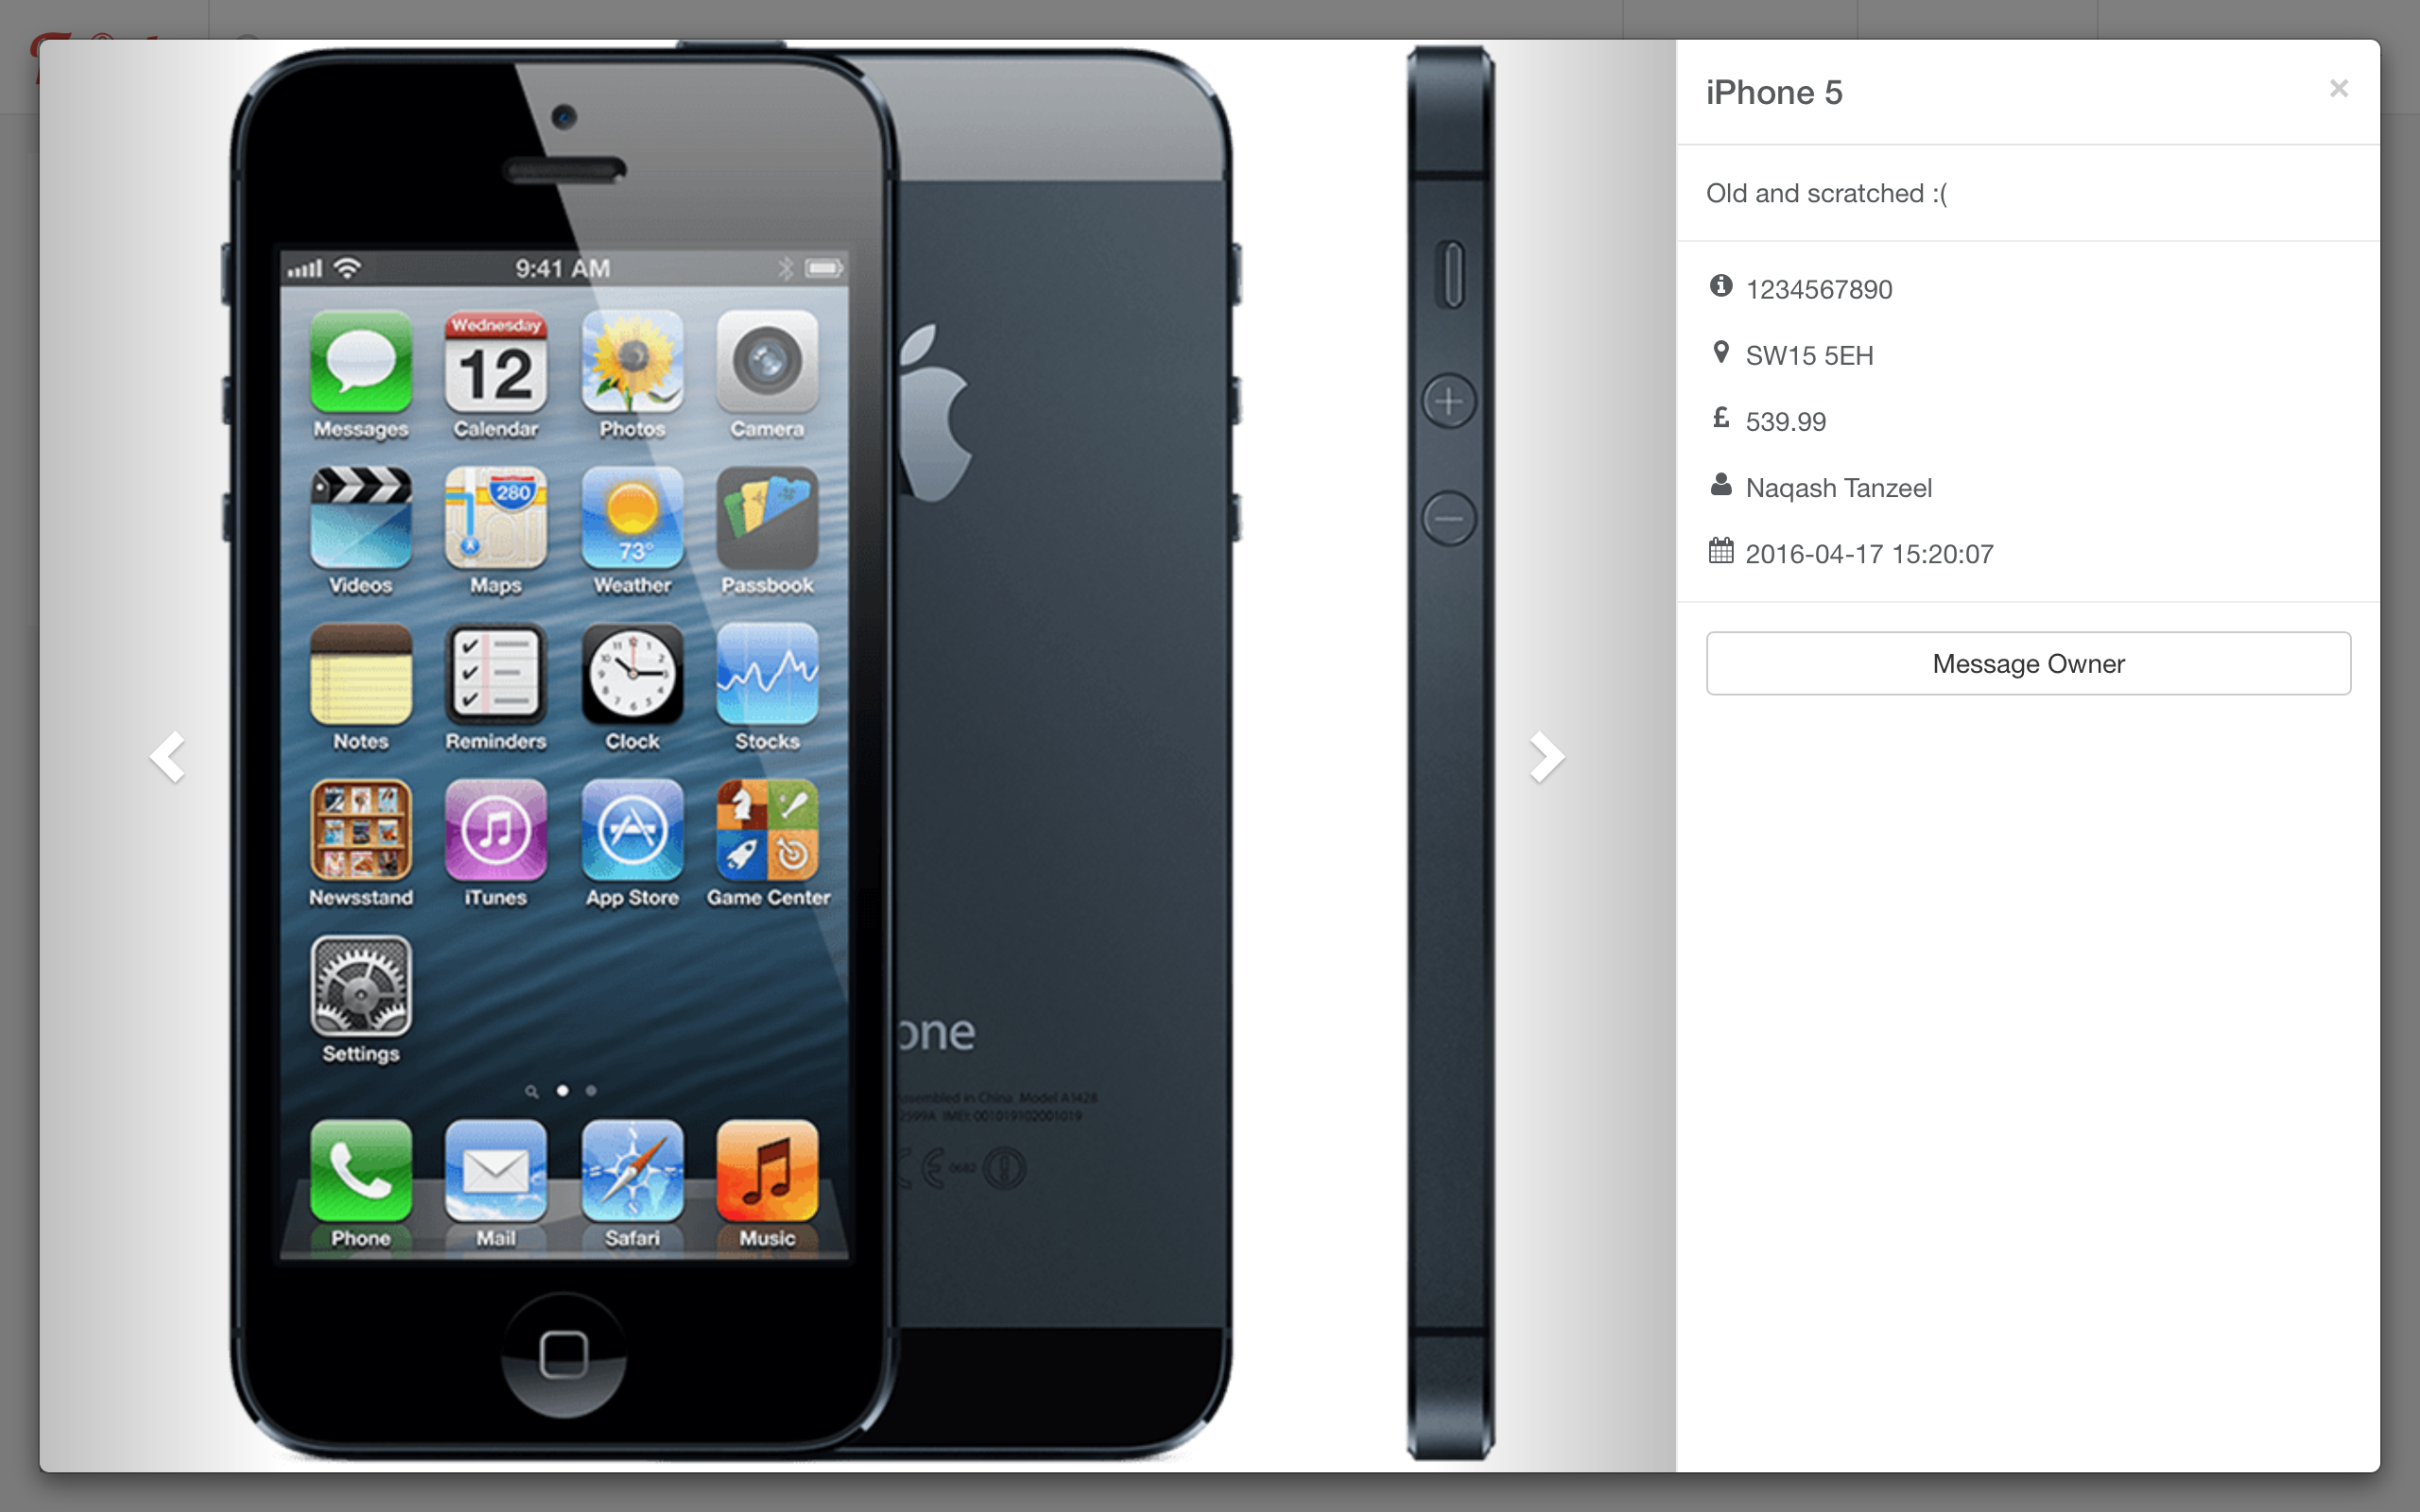
\includegraphics[width=1.0\textwidth]{images/Frisk/View_Item}
	\caption{View Item Modal} \label{fig:View_Item}
\end{figure}

\subsection{Dashboard}
The dashboard follows a different layout to the previously discussed page and hence the implementation details are entirely different. The layout still extends the base master view, to inherit the stylesheets and scripts, for the basic functionality. The dashboard is only available to authenticated users and this section discusses the implementation of the dashboard functionality. The assumption that the user data is always available due to the authentication middleware allowing requests to reach the dashboard.

\subsubsection{Commonalities}
As with pages, the dashboard offers a lot of functionality that is common across most of the pages. The dashboard actually provides a much more complex user experience and hence it is important to abstract this functionality. The three main aspects of the dashboard which are kept common are the design, header and sidebar.

\paragraph{Design}
The layout and design of the dashboard was implemented from scratch without any templates or code from third-parties. The design mostly inspired from common dashboard layouts which include a sidebar. However one key influence on the dashboard design was the canvas web application for managing university assignments \cite{Canvas:Home}. The sidebar colour and the top header on pages was mostly inspired from this application. Once again, all the icons used were provided by the FontAwesome repository and the Bootstrap Glyphicon font. The same font as the front end was used to provide a consistent experience and a sense of familiarity even though a completely different design has been implemented.

The design consists of a sidebar which contains all the navigation links along with a header bar. The header bar itself has several components including a title, actions and a crumb bar but these will be discussed separately. Finally the dashboard master layout provides a wrapping container than limits the edges of the content and all dashboard pages implement their own content for this container.

\paragraph{Header}
The header consists of three major components which include the title, the page action and the crumb bar. The design for these items is contained within the master layout file and is not changed based on the page. The extending child view can using the \emph{@section} directive to set the title of the page. Similarly, the page action is an unordered list to which items can be added on per page basis. These items are essentially links to accomplish tasks on the page. For example, on the saved locations page the user can create a new location so a 'new' action is added. The final component is the crumb bar which is automatically generated by splitting the url components. However, the user may change the final link in the crumb bar by overriding it inside a child view.

\begin{figure}[H]
	\centering
	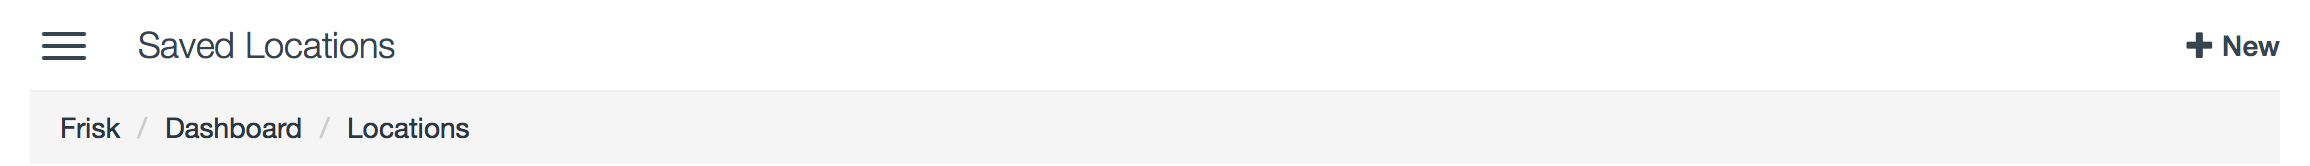
\includegraphics[width=1.0\textwidth]{images/Frisk/Dashboard_Header}
	\caption{Dashboard Header} \label{fig:Dashboard_Header}
\end{figure}

There is an additional feature which is not visible in figure \ref{fig:Dashboard_Header}. This is the notification slider that appears slides down a notification needs to be displayed to the user without refreshing the page. The notification slider can be brought into view using a global JavaScript function which takes a notification message and type as a parameter. The type is used to determine the colour where error, warning and success are red, yellow and green respectively. This is the man method of providing notifications to the user for any tasks that involve AJAX, such as deleting items or locations.

\paragraph{Sidebar}

The sidebar is the main source of navigation within the dashboard. It provides links to the main components of the system which them further implement links for their components in the header. The user is able to hide the sidebar using the toggle in the header. On a desktop device, when the sidebar is visible, the container is shrunk to accommodate the sidebar whereas on a mobile device the entire container is shifted to the side until the user is done with the sidebar and hides it again. The latter approach was taken for mobile devices due to the lack of room available and thus shrinking the content would distort it completely and make the user interface seem cluttered.

\begin{figure}[H]
	\centering
	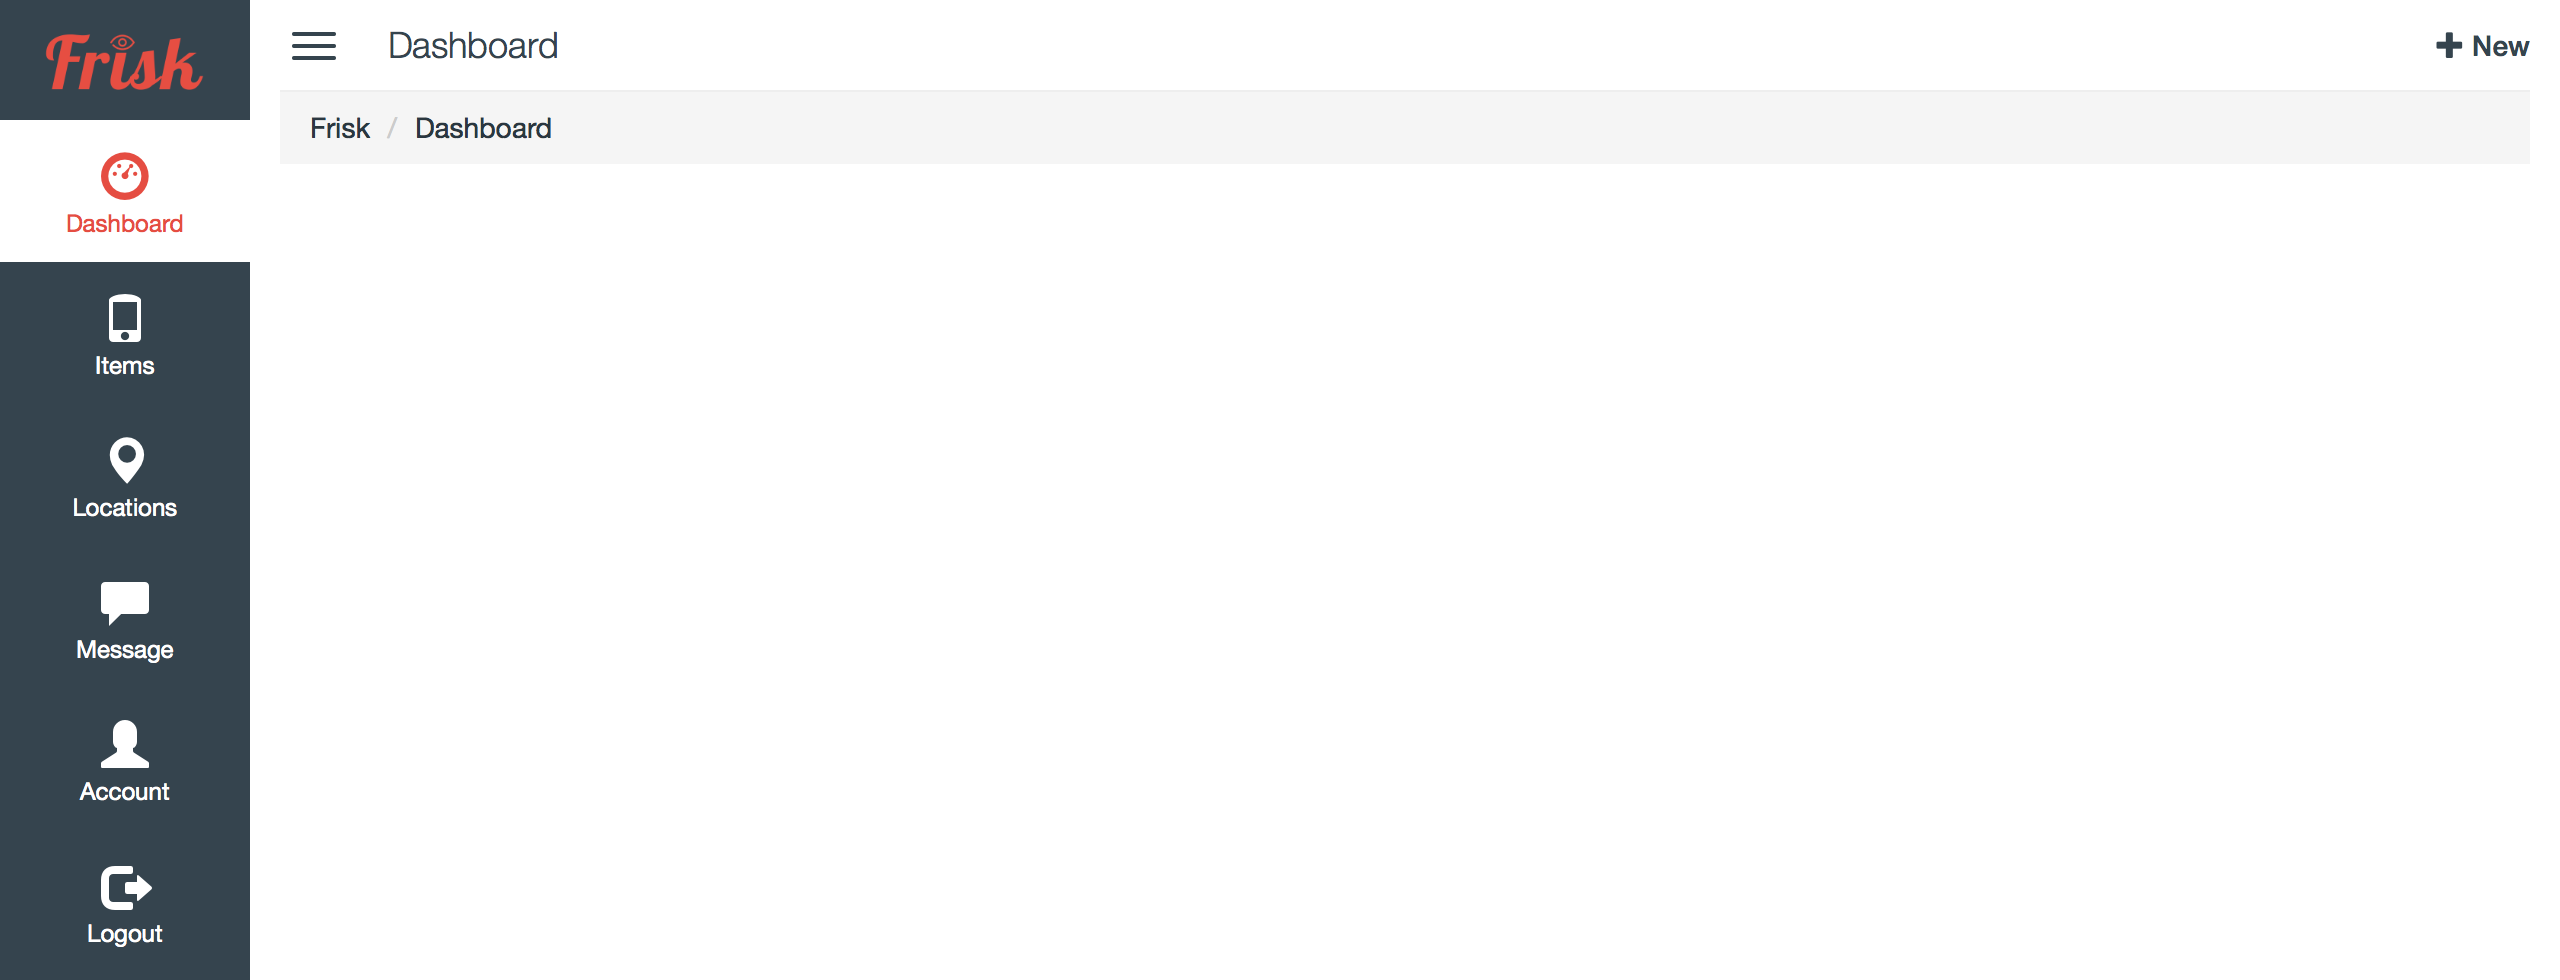
\includegraphics[width=1.0\textwidth]{images/Frisk/Dashboard_Sidebar}
	\caption{Dashboard Sidebar} \label{fig:Dashboard_Sidebar}
\end{figure}

As can be seen in figure \ref{fig:Dashboard_Sidebar} the active link is highlighted without a white background and orange text whereas the other links have a default background and white text. This is accomplished by executing JavaScript  code, when the page finishes loading, which checks the current URL against the URL of all the links in the navigation. The link which matches the URL exactly or is the closest match is assigned the \emph{.active} css class.

\subsubsection{Locations}
The locations page allows the user to view all the locations they have saved onto their profile. The page is relatively simple with default header and a link to create new location (see figure \ref{fig:Dashboard_Header}). The locations are displayed on the page as tiles, similar to the search results. Each tile is a map with the location marked on it using a map marker. The title additionally has a label which states the first line of the address along with the postcode. The design for the location tiles can be seen in figure \ref{fig:Location_Tiles} where as the design for the overall locations page can be seen in figure \ref{fig:Dashboard_Locations}. Each row can accommodate 3 tiles on a desktop device but this number is reduce to one on smaller devices.

\begin{figure}[H]
	\centering
	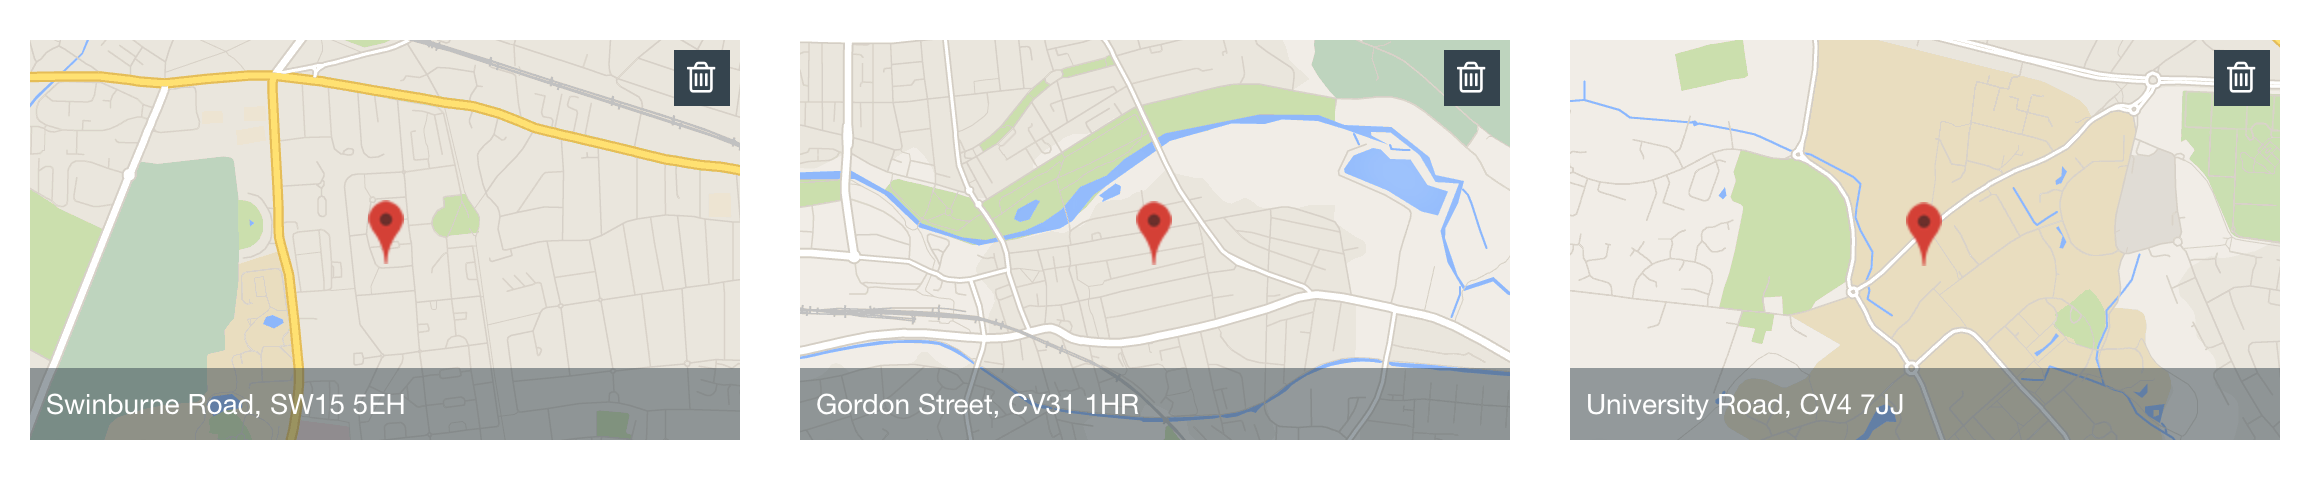
\includegraphics[width=1.0\textwidth]{images/Frisk/Location_Tiles}
	\caption{Tiles for Saved Locations} \label{fig:Location_Tiles}
\end{figure}

The map for each tile is generated using the same approach as with the explore and the home page. An element is created for each map which is set to a fixed height. The element is then assigned the css class \emph{.map} which identifies all elements that will contain a map. Additionally, two custom attributes are set on the element which contain the latitude and longitude of the map centre and the coordinate of the marker. Once the page is loaded a script collects all the elements and generates the map for each element using the coordinates in the attributes.

\paragraph{Registering a New Location}
Locations need to be created and deleted often as they form the basis of the functionality offered by the system. Each item may be stored in a different location and when stolen they may or will be stolen at different locations. With this in mind, the location process was simplified as much as possible so that a new location could be created within just seconds. In order to achieve this, the user was provided with two simple options for creating an option either using their postcode or their current location by the browser. If all else fails, the user can resort to a manual address input for inserting a custom location.

\begin{figure}[H]
	\centering
	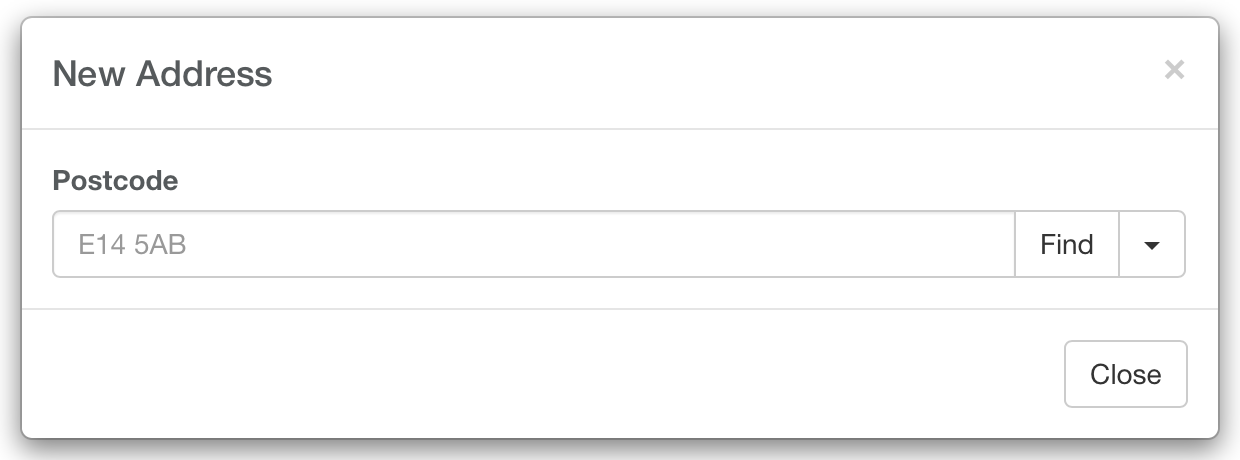
\includegraphics[width=1.0\textwidth]{images/Frisk/Dashboard_Find_Location}
	\caption{Find Location Form for Finding Registering a New Location} \label{fig:Dashboard_Find_Location}
\end{figure}

The modal shown in figure \ref{fig:Dashboard_Find_Location} can be brought up, by clicking the new link in the header, on the locations page. The form provides a single input for the users to enter the postcode of the location they wish to register. Once the user enters a postcode, they can click the find button to automatically retrieve the full address for the location (minus the door number). The address is retrieved using a custom class written in JavaScript which wraps the Google Maps GeoCoding API. The wrapper starts by sending a geocode request to the Google Maps with the postcode and then captures the JSON response output by the server. This response contains various details about the address, including full address and coordinates. The necessary details are filtered out from the response and used to populate the address form automatically using JS. Once the address has been resolved and the form has been populated, the address lookup form is replaced with the address form which the user can verify and amend before saving the location.

Alternatively, the user can choose to retrieve their address using their current coordinates. A similar process to postcodes is used for decoding addresses from coordinates. The system send a request to the Google Maps server but this time, instead of the postcode, the coordinates are sent to the server and the response is captured, filtered and used to populate the form. Once the user has verified their address they can press the save button which saves the address in the database using an AJAX form submission. The serve captures the data from the submitted from the form and before it is appended to the database, the current users id is attached to it so it can be associated with the user. A notification similar to the one in figure \ref{fig:Notification_Success} is displayed to the user to let them know that the address has been saved.

\paragraph{Deleting a Location}
Deleting locations is a simple one click procedure. Each tile has an attached delete button in the top right corner which allows the user to asynchronously delete a location without having to refresh the page. The delete request is sent to the server which verifies the user requesting the delete and processes the request accordingly. If the system is unable to process the request then an error is returned to the user which is displayed in a notification to the user (see figure \ref{fig:Notification_Error}). An error can be returned when the user requesting the delete is not the one associated with the location or if the location being deleted is being used by one or more items which have not yet been deleted. However, if the item is deleted then it is immediately removed from the page through the use of JavaScript DOM manipulation and the tiles are adjusted to fill the empty space.

\begin{figure}[H]
	\centering
	\begin{subfigure}[t]{1\textwidth}
		\centering
		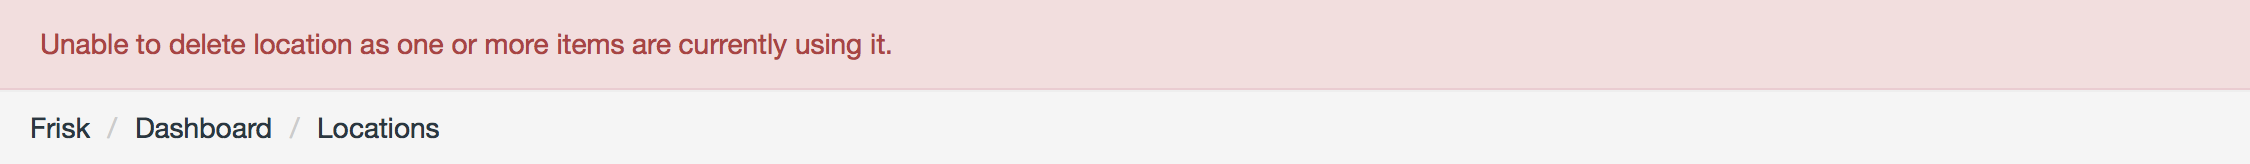
\includegraphics[width=1.0\textwidth]{images/Frisk/Notification_Error}
		\caption{Error Notification for Deleting a Location}\label{fig:Notification_Error}		
	\end{subfigure}
	\quad
	\begin{subfigure}[t]{1\textwidth}
		\centering
		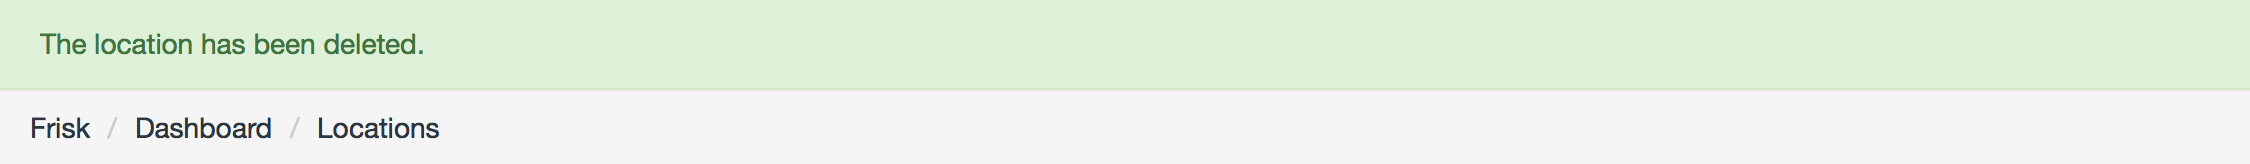
\includegraphics[width=1.0\textwidth]{images/Frisk/Notification_Success}
		\caption{Success Notification for Deleting a Location}\label{fig:Notification_Success}
	\end{subfigure}
	\caption{Success and Error Notifications for Deleting a Location}\label{fig:Notifications}
\end{figure}

\subsubsection{Items}
The items page is very similar to the locations page, where all the items registered to the user are presented as tiles. The background of each tile is set to the cover image provided by the user when creating the item and the caption at the bottom is the name provided by the user. The main difference on the items page is that each item tile also has an associated edit link as well as a delete link. The design for the items page can be seen in figure \ref{fig:Dashboard_Items}. A closeup of the category tabs and item tiles is also available in figure \ref{fig:Item_Tiles}.

\begin{figure}[H]
	\centering
	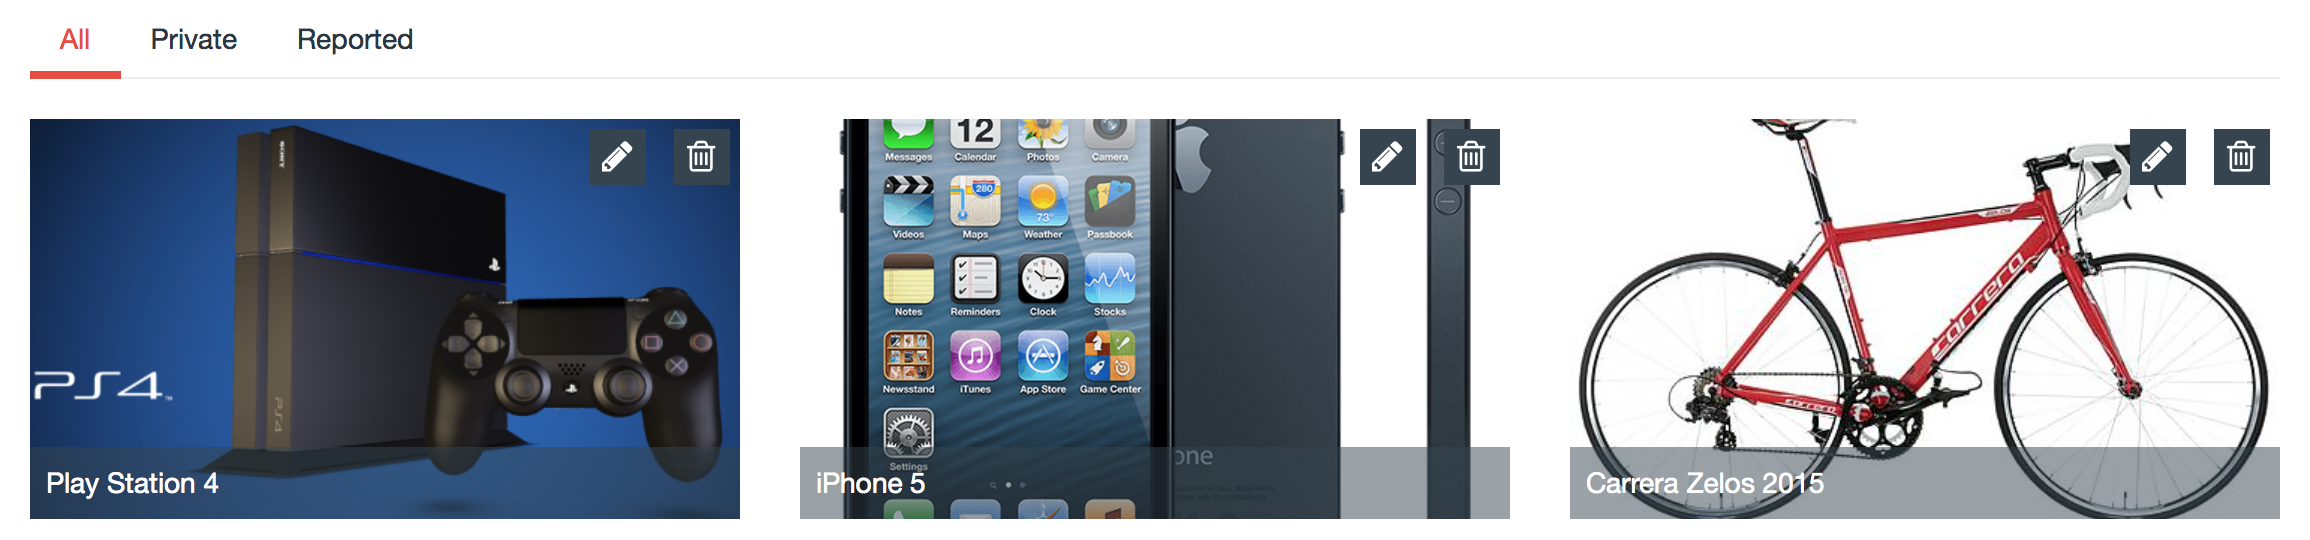
\includegraphics[width=1.0\textwidth]{images/Frisk/Item_Tiles}
	\caption{Category Tabs and Tiles for Registered Items} \label{fig:Item_Tiles}
\end{figure}

In addition to the difference mentioned previously, the items are split into three categories and the user can either view all the items, only ones that have been reported as lost or stolen, or items that are still in their private vault. The code shown creates a Laravel collection with three different keys, one for each of the three categories on the page, where each key is mapped to an empty array. The items returned by the query are also returned as a Laravel collection of Models and thus a \emph{groupBy} function can be used to group the results into the three categories. The two collections are then merged together and the result is a collection with keys where the key maps to an array of Models if any exist or an empty array.

\begin{lstlisting}[language=php]
	$items = collect(['all' => $items, 'private' => [], 'reported' => []])->merge($items->groupBy(function($item) {
            return $item->stolenRecord ? 'reported' : 'private';
        }));
\end{lstlisting}

\paragraph{Creating and Editing an Item}

Creating an item is a simple procedure which can accomplished through the use of a form with some required and optional inputs. The user can create a new item by clicking the 'new' link in the header which redirects the user to the create item page. On this page are several fields which the user is required to fill in before they can proceed to the next step. The exact same view is returned by the edit item function but this time the fields are populated with the details of the item the user is editing. Additionally the image field is hidden on the edit page as the image can be edited using the resources page. The form can be seen in figure \ref{fig:Dashboard_Create_Item}.

\begin{figure}[H]
	\centering
	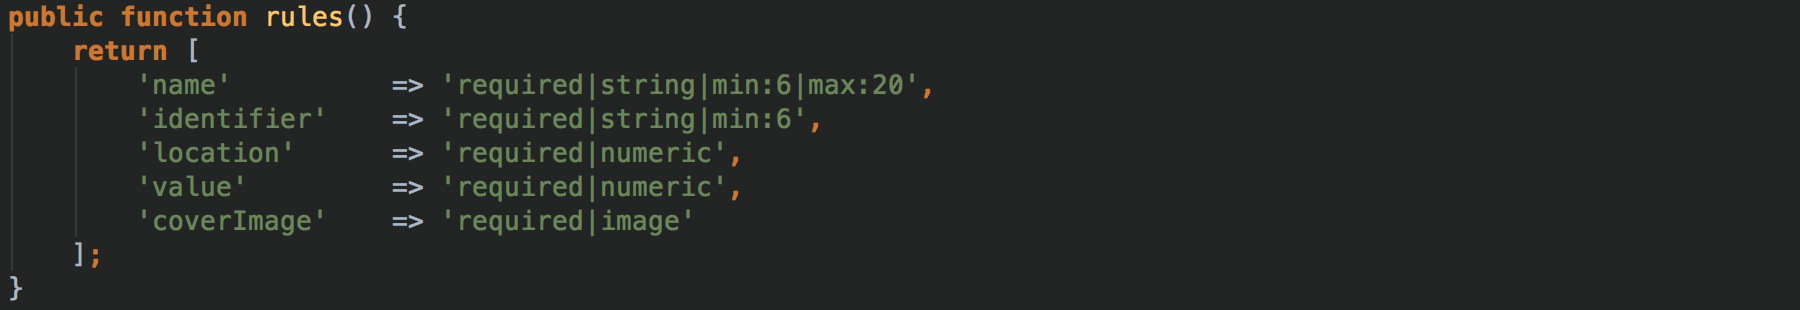
\includegraphics[width=1.0\textwidth]{images/Code/Validation_Rules}
	\caption{Category Tabs and Tiles for Registered Items} \label{fig:Validation_Rules}
\end{figure}

All the fields are validated using the Laravel request class which can be extended to provide validation rules. These validation rules define things such as the type of input, the length and the accepted values (see figure \ref{fig:Validation_Rules} for example). The request is automatically validated before the route closure is called and if validation fails the error can be printed to the user as shown in figure \ref{fig:Item_Errors}.

\begin{figure}[H]
	\centering
	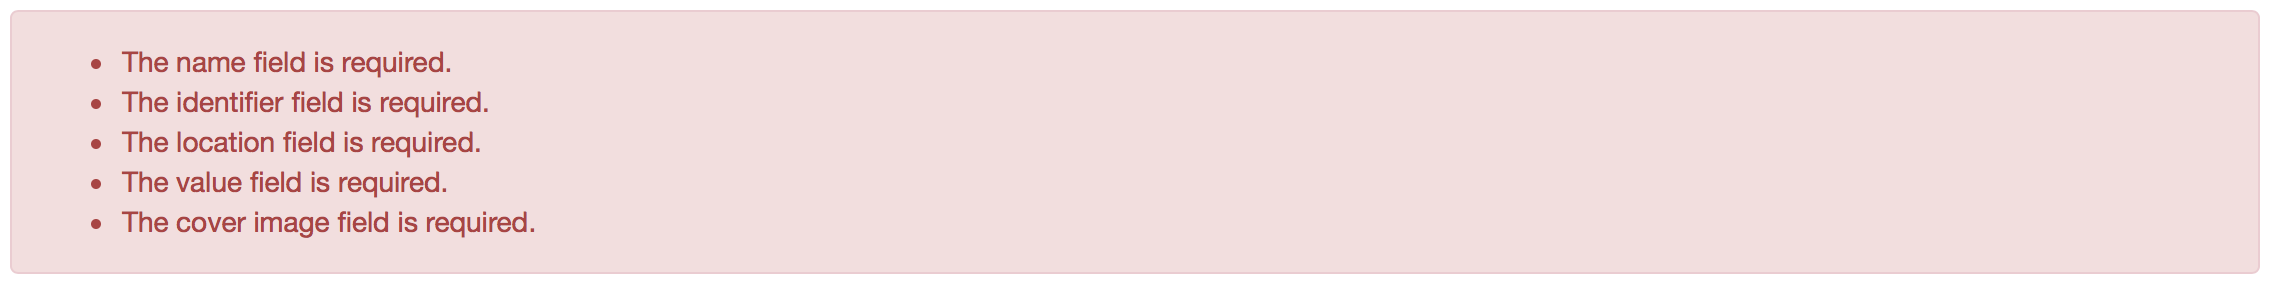
\includegraphics[width=1.0\textwidth]{images/Frisk/Item_Errors}
	\caption{Validation Errors when Creating an Item} \label{fig:Item_Errors}
\end{figure}

\paragraph{Deleting an Item}
Deleting items follows the exact same procedure as deleting locations. A delete button is located in the top right corner of each tile which the user can click to initiate an AJAX request for deleting the item and upon success the item would be removed from the page. This meant that there would be repeated code for deleting items and deleting locations as both operations are the same but just take different parameters. It seemed logical to abstract this process into a generic delete button which could be applied to any element on the page and would functional without any additional code for certain circumstances.

\begin{lstlisting}
	<a class="delete" data-for="#location-{{ $location->id }}" data-target="{{ route('locations::delete', [$location->id]) }}" data-token="{{ csrf_token() }}">
		<i class="fa fa-trash-o"></i>
	</a>
\end{lstlisting}

The code shows a generic delete button that supports the deletion of any element from the database through the use of \emph{data-target} attribute which specifies the end point for deletion. Additionally, using the \emph{data-for} attribute, the user specifies the element on the page that must be removed once the deletion request has been successfully completed. Upon page load, a JavaScript is bound to the click event of every element with the delete class and the code for this is shown in figure \ref{fig:Generic_Delete}.

\begin{figure}[H]
	\centering
	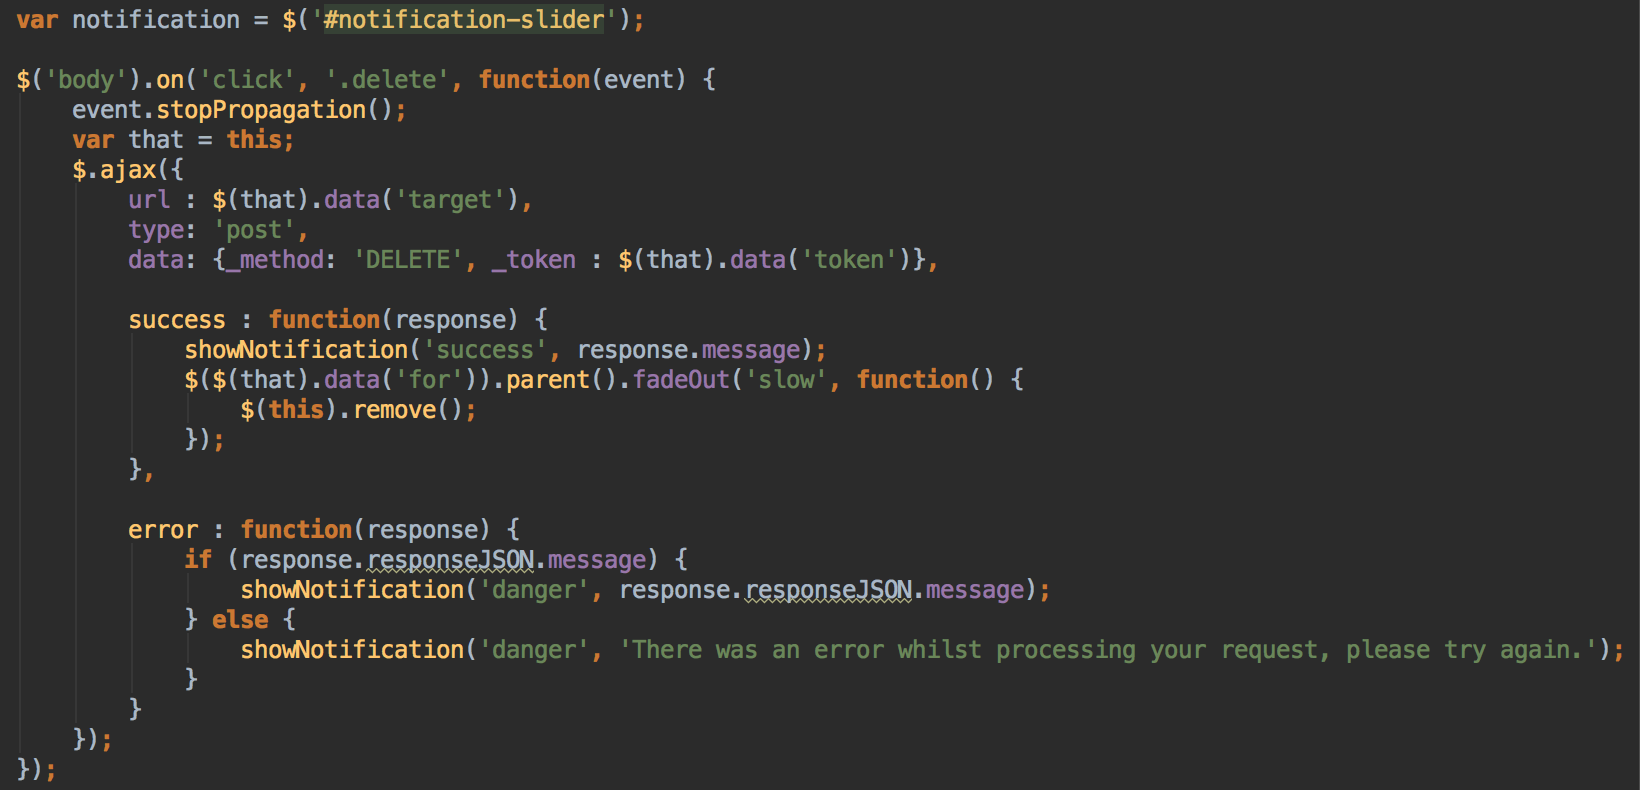
\includegraphics[width=1.0\textwidth]{images/Code/Generic_Delete}
	\caption{Code for the Generic Delete Button} \label{fig:Generic_Delete}
\end{figure}

The event works by submitting an AJAX request to the URL specified and captures the deletion response from this URL. If the element is successfully deleted then a success notification such as the one in figure \ref{fig:Notification_Success} is shown the user and the item is deleted. However, if there is an error deleting the item then the error message, if one is provided, or a generic message is displayed to the user in a notification. Additionally the user can also delete the item using then actions dropdown menu on the edit page which simply uses a redirect to delete the item.

\paragraph{Reporting an Item as Lost or Stolen}
Reporting the item as lost or stolen as well as being able to report it as recovered will be a commonly used feature and for this reason it needs to be made as simple as possible. The procedure for both these cases is fairly similar. The user can achieve either of these tasks by firstly visiting the edit item page then switching to the report tab using the navigation toggles under the header. Once on the report tab, if the user has not already, they can mark the item as lost or stolen. In order to do this, the user must select a location, from one of their registered location, where the item was stolen from. This will create a new entry in the stolen item table which links to the item itself using the id. If the item has already been reported as lost or stolen then the user can simply click the mark as recovered button to delete the theft record.

\begin{figure}[H]
	\centering
	\begin{subfigure}[t]{0.45\textwidth}
		\centering
		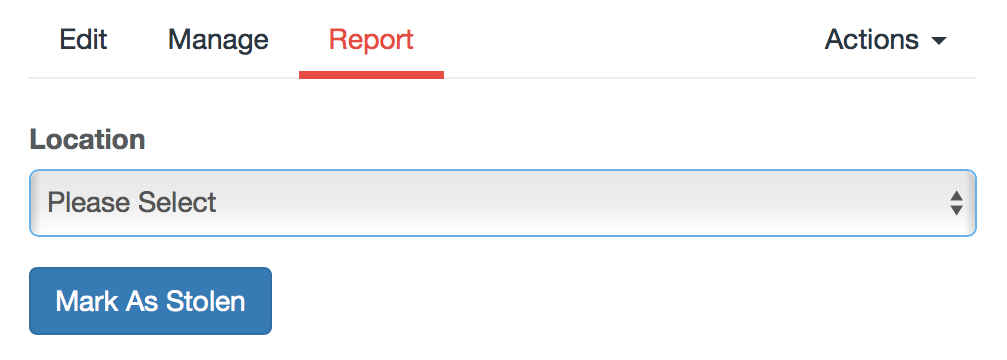
\includegraphics[width=1.0\textwidth]{images/Frisk/Report_Stolen}
		\caption{Report as Stolen}\label{fig:Report_Stolen}		
	\end{subfigure}
	\quad
	\begin{subfigure}[t]{0.45\textwidth}
		\centering
		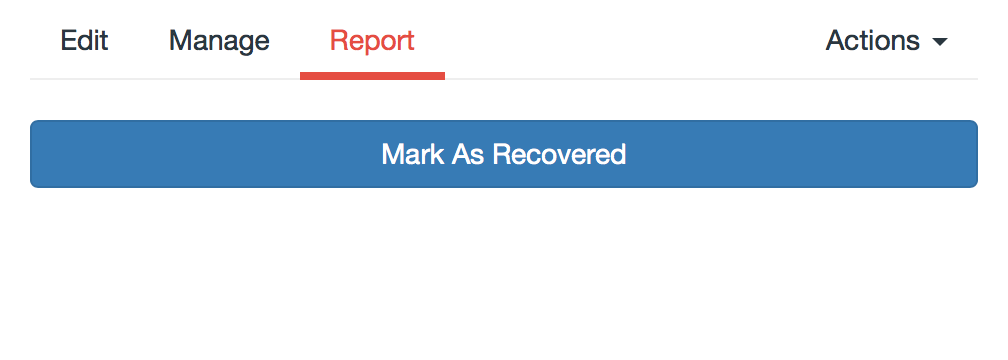
\includegraphics[width=1.0\textwidth]{images/Frisk/Report_Recovered}
		\caption{Mark as Recovered}\label{fig:Report_Recovered}
	\end{subfigure}
	\caption{Toggling the Item Between Private and Reported}\label{fig:Notifications}
\end{figure}

\subsubsection{Resources}

Users need to know what the item looks like in order to identify it if they ever come across it. This need is fulfilled by the image field when creating a new item but additional images can be provided through the resources, which allows the user to upload image, documents and other file types. Resources are associated with an item and cannot exist without one and thus the resources for an item can be managed by clicking the resources tab on the edit item page. Similar to the items the resources are, displayed as tiles, grouped into all and private or public. The tile shows a preview of the image or certain filetypes as the background and the custom alias assigned by the user as the caption. Figure \ref{fig:Item_Resources} shows the resources tab with some resources in the all category.

\begin{figure}[H]
	\centering
	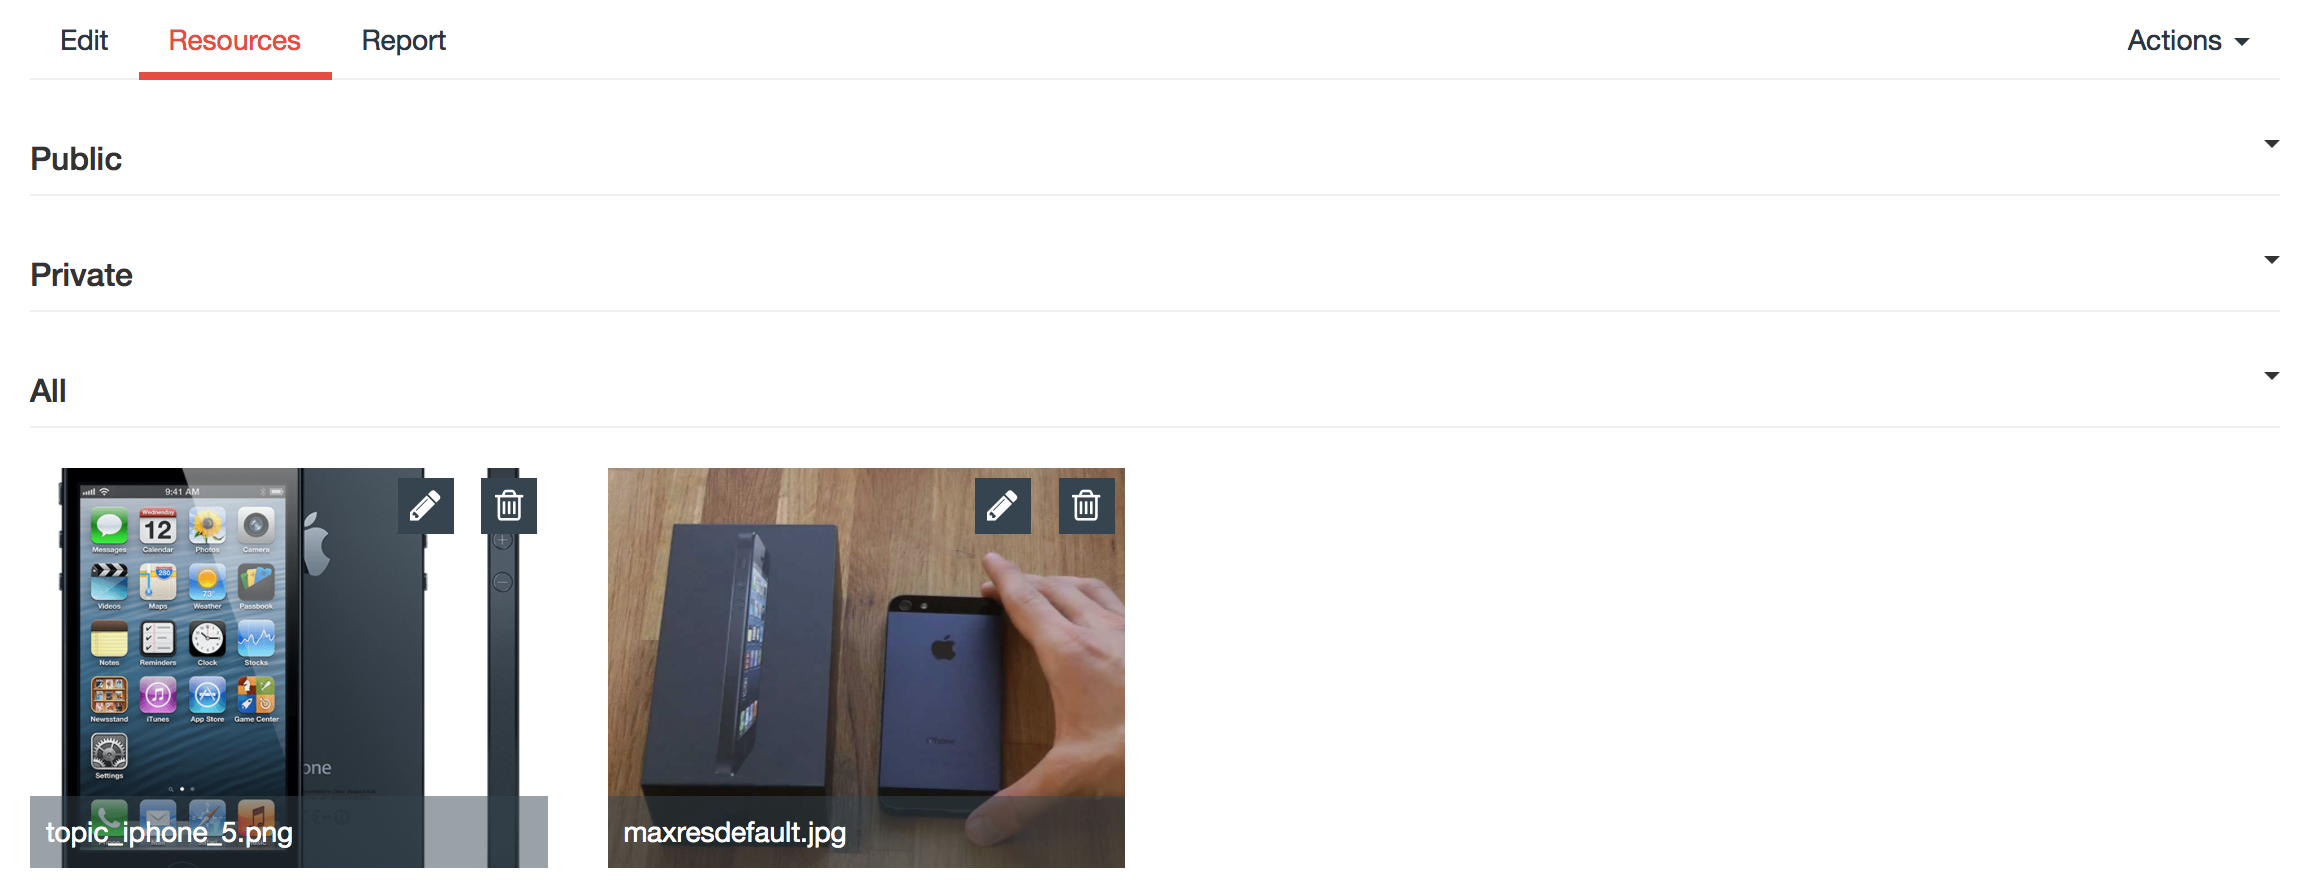
\includegraphics[width=1.0\textwidth]{images/Frisk/Item_Resources}
	\caption{The Resources Tab for an Item with All Category Expanded} \label{fig:Item_Resources}
\end{figure}

\paragraph{Uploading and Editing a Resource}
The upload process is all completed through JavaScript meaning the user does not need to refresh the page at all when uploading resources. In order to upload resource the user can click upload from the actions drop down in the top right corner of the navigation tabs menu. This presents a Bootstrap modal with a DropZone nested in the body \cite{DropZone:Home}. The user can upload a resource of any type by either clicking or dragging items onto the the DropZone container. Once uploaded the user can simply close the modal and the resources are automatically saved.

\begin{figure}[H]
	\centering
	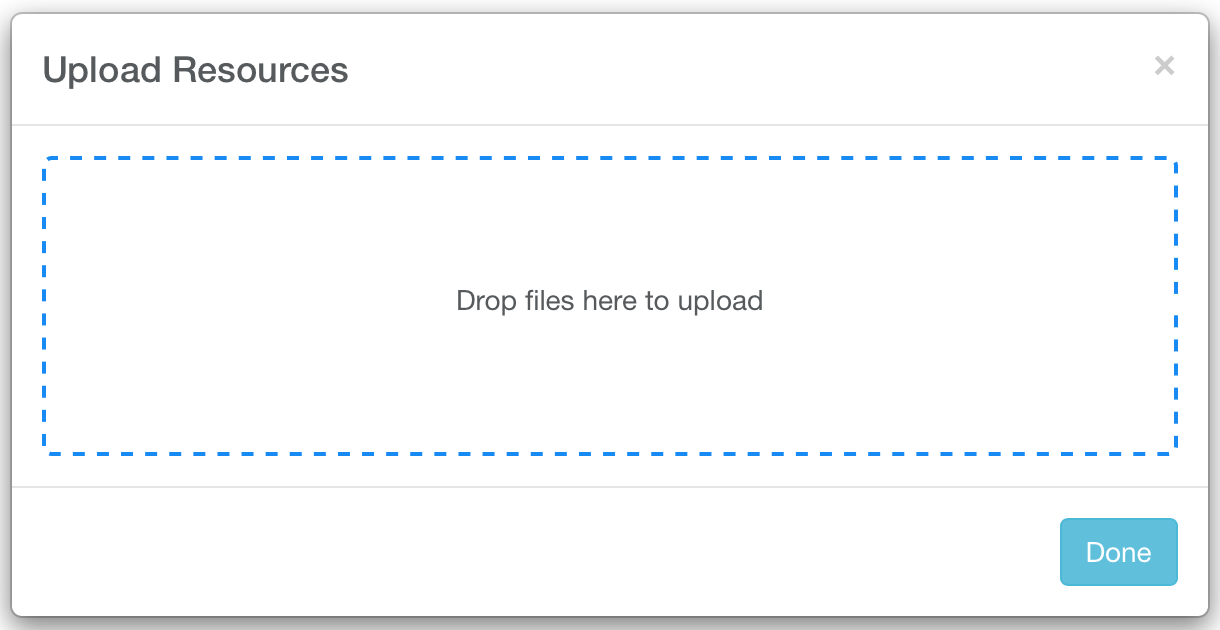
\includegraphics[width=1.0\textwidth]{images/Frisk/Upload_Resource}
	\caption{Upload Resource Modal with DropZone} \label{fig:Upload_Resource}
\end{figure}

DropZone uploads by submitting each resource individually using form attributes, implemented as part of HMTL 5. Each resource is individually processed by the server side and validation is performed to insure the resource is valid. These resources are stored in the appropriate directory for the user and the item.

\begin{lstlisting}
	if ($success) {
            $fileName = $file->getFilename() . '-' . time() . '.' . $file->getClientOriginalExtension();
            $storagePath = 'uploads/' . Auth::user()->storagePath() . '/' . $item->storagePath();
            $file->move($storagePath, $fileName);
            $success = $item->resources()->save(new Resource([
                'alias' => $file->getClientOriginalName(),
                'name'  => $fileName,
                'path'  => $storagePath,
                'type'  => str_contains($file->getClientMimeType(), 'image') ? Resource::$PRIVATE : Resource::$OTHER
            ]));
        }
\end{lstlisting}

The code for the validation and moving of the files can be seen above. One important factor to note is that the method uses the files mime type to determine what kind of resource it is and this is stored in the database as an integer value where private is 1, public is 2 and other is 3. 

\begin{figure}[H]
	\centering
	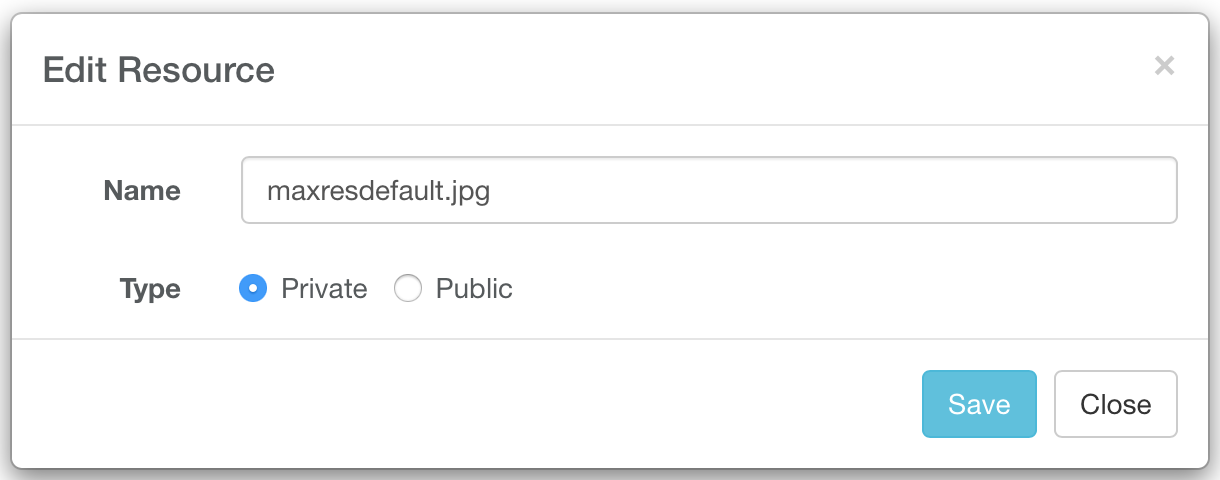
\includegraphics[width=1.0\textwidth]{images/Frisk/Edit_Resource}
	\caption{Edit Resource Modal} \label{fig:Edit_Resource}
\end{figure}

When an image is uploaded it's firstly stored as type private and the filename is used as the alias. The type can later be toggled between private and public for images, as long as there is at least one public image, and the alias can be changed to a useful identifier for the user.

\paragraph{Deleting a Resource}
Deleting a resource uses the same generic approach as items and locations which has been discussed previously. The one difference on the server side of the implementation is that a resource cannot be deleted if it is the last public resource, implying that it is the last remaining image, as this is required for the search feature. A simple check is performed before deleting the resource to ensure this and an error is returned if the check fails.

\begin{lstlisting}[language=php]
	$success = $resource && $resource->item->user_id == Auth::user()->id && ($resource->type != Resource::$PUBLIC || $publicResources->count() > 1) && $resource->delete();
\end{lstlisting}

\subsubsection{Messages}
The messages component was the last component to be integrated, due to its reliance on locations, items and and implementation of stolen items. The messages page is, in some ways, similar to the other pages available on the dashboard but at the same time follows a completely different layout. The header is immediately followed by a tab navigation which allows the user to switch between received and sent messages. The messages are then displayed in a table and email inbox like format where the user can see the subject, sender and time of the message along with a reply and delete link. Some of these properties are hidden on the mobile version due to lack of space. Notice that there is no new button in the header, the user is not allowed to compose new messages to a specified user as this would result in spam, the only way to contact a user is through the search and explore page. Figure \ref{} shows the inbox view of the messages but the full design can be seen in figure \ref{fig:Dashboard_Messages}.

\begin{figure}[H]
	\centering
	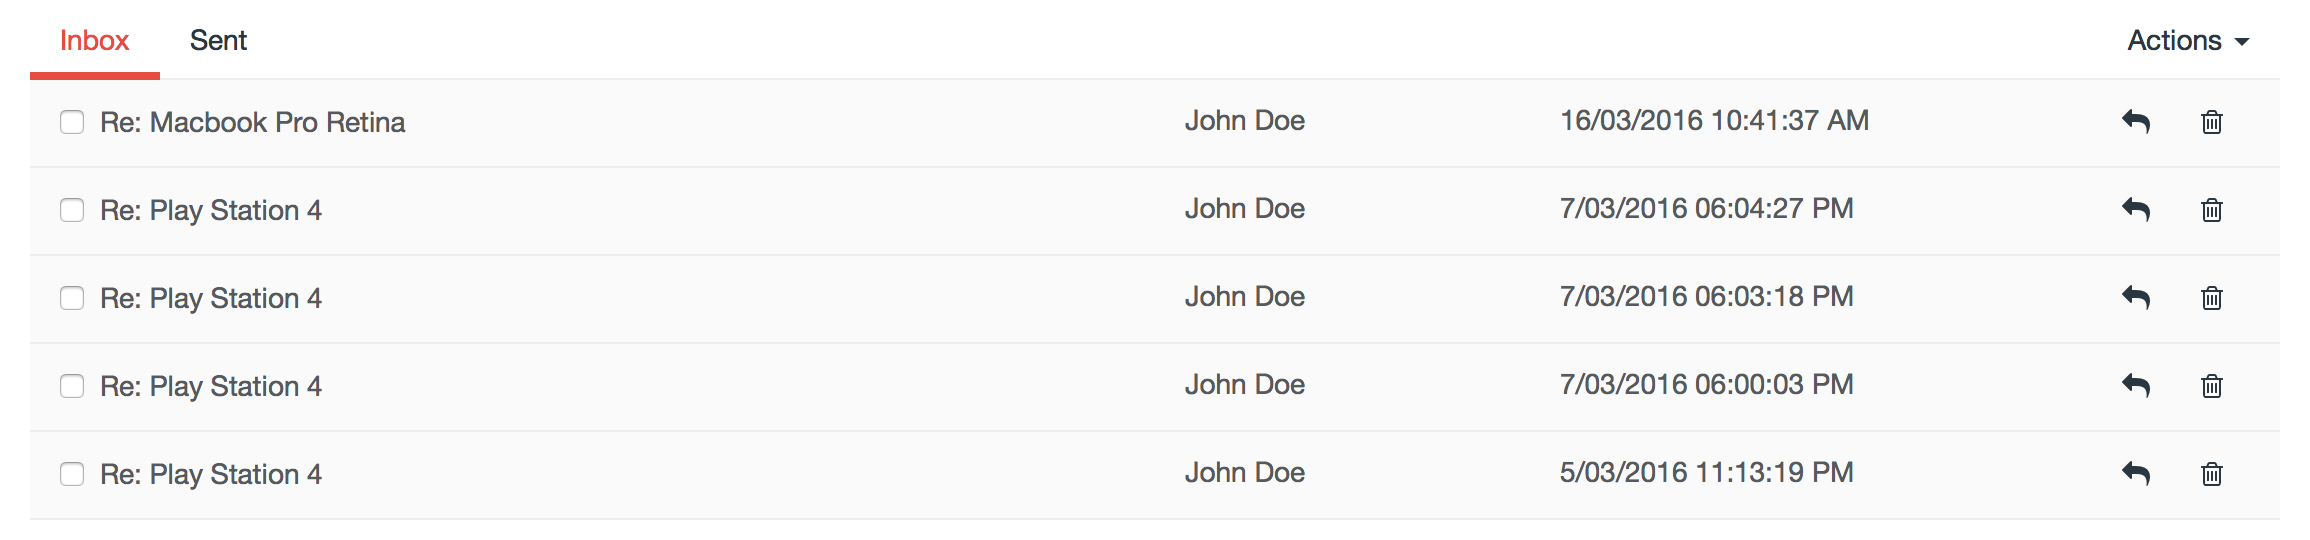
\includegraphics[width=1.0\textwidth]{images/Frisk/Inbox}
	\caption{Messages Inbox with Table View} \label{fig:Inbox}
\end{figure}

In order to display messages in groups and filter out the deleted messages, the messages tables needed to be join onto the deleted messages table. The results were then grouped using the Laravel collection \emph{groupBy} method, similar to that of items. The code for this can be seen in figure \ref{fig:Messages_Code}

\begin{figure}[H]
	\centering
	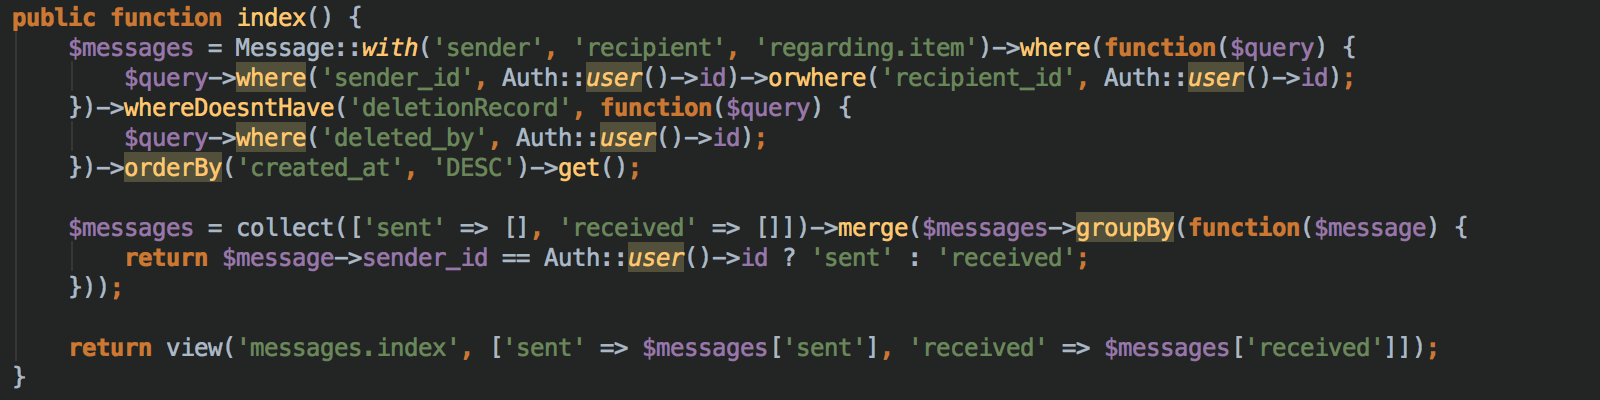
\includegraphics[width=1.0\textwidth]{images/Code/Messages}
	\caption{Code for Grouping Messages and Filtering Deleted Messages} \label{fig:Messages_Code}
\end{figure}

\paragraph{Viewing, Creating and Replying to Messages}
The user can view a message simply by clicking one of the rows on the messages page. This will redirect the user to the view message page where a reply link is provided in the header to allow the user to reply to a message. The design for this page is similar to that of the create and reply page but instead of input boxes, plain labels are used. The user can create a message by clicking the message owner link on the view item modal, accessible through the search and explore page. This will redirect the user to the create message page where the recipient and subject fields are automatically populated but the user can enter a custom message. The same form is used for the reply page but the sender of the original message is assigned as the recipient of the reply. The design for this can be seen in figure \ref{fig:Dashboard_Messages}.

\begin{lstlisting}[language=php]
	if ($message->sender_id == Auth::user()->id || $item->trashed())
            return redirect()->route('messages::index');
\end{lstlisting}

Protecting users privacy as well as protecting them from spam is important. If the user attempts to access the message form once the item has been marked as recovered, either by visiting the url or click reply on an existing message, they are redirect back to the messages page. This functionality is demonstrated by the quoted code.

\paragraph{Deleting Messages}
There are two ways the user can delete a message from either their inbox or their sent items. One way to delete a message is using the generic delete button, similar to locations and other pages, provided in the actions column of each message. The alternative method for deleting messages is using the delete option in the actions dropdown menu. This feature allows the user to delete multiple messages by selecting the checkbox next to each message they wish to delete. The process works by finding all messages for which the checkbox is in a checked state. Once the messages are found they can simply be deleted by locating their associated delete button and triggering a click on this using JavaScript. Once the message is deleted, a notification is returned to the user notifying them and the message is removed from the list.

\begin{lstlisting}[language=php]
	$message = Message::find($id);
	$success = $message && ($message->sender_id == Auth::user()->id || $message->recipient_id == Auth::user()->id);
	$record = new DeletedMessage([
			'deleted_by'    => Auth::user()->id
        ]);
	$success = $success && $message->deletionRecord()->save($record);
\end{lstlisting}

The problem encountered for messages was that if a single user deletes the message and the record in the database is soft deleted then the message would be removed for both users, as there is no way of identifying the user that requested the delete. A solution for this was devised and implemented using the code quoted above. The solution involved a new table which would map each message to each user that requests a deletion, essentially acting as a pivot table between the users and messages table (see line 3 of code). This meant that only messages for which there is no row in the deleted messages table, with the current users id in the deleted\_by column, would be fetched.

\subsection{Responsive Design}
The use of mobile devices to surf the web is growing at an astronomical pace, but unfortunately much of the web isn't optimised for those mobile devices. Mobile devices are often constrained by display size and require a different approach to how content is laid out on screen \cite{GoogleDev:Responsiveness}. However since the introduction of CSS media queries and frameworks such as Bootstrap, responsive web applications are becoming an ever increasing site on the internet due to their ability to serve multiple devices \cite{Bootstrap:Home}. Before we delve into the Bootstrap framework and it's column layout it's important to understand what media queries are and how they work, as custom media queries will need to be used throughout the application. Pete LePage, a we development advocate, described media queries as "simple filters that can be applied to CSS styles. They make it easy to change styles based on the characteristics of the device rendering the content, including the display type, width, height, orientation and even resolution." \cite{GoogleDev:Responsiveness}.

Bootstrap easily and efficiently scales your websites and applications with a single code base, from phones to tablets to desktops with CSS media queries \cite{Bootstrap:Home}. In order to achieve this, Bootstrap implements a responsive, mobile first fluid grid system that appropriately scales up to 12 columns as the device or viewport size increases \cite{Bootstrap:Grid}.

\begin{figure}[H]
	\centering
	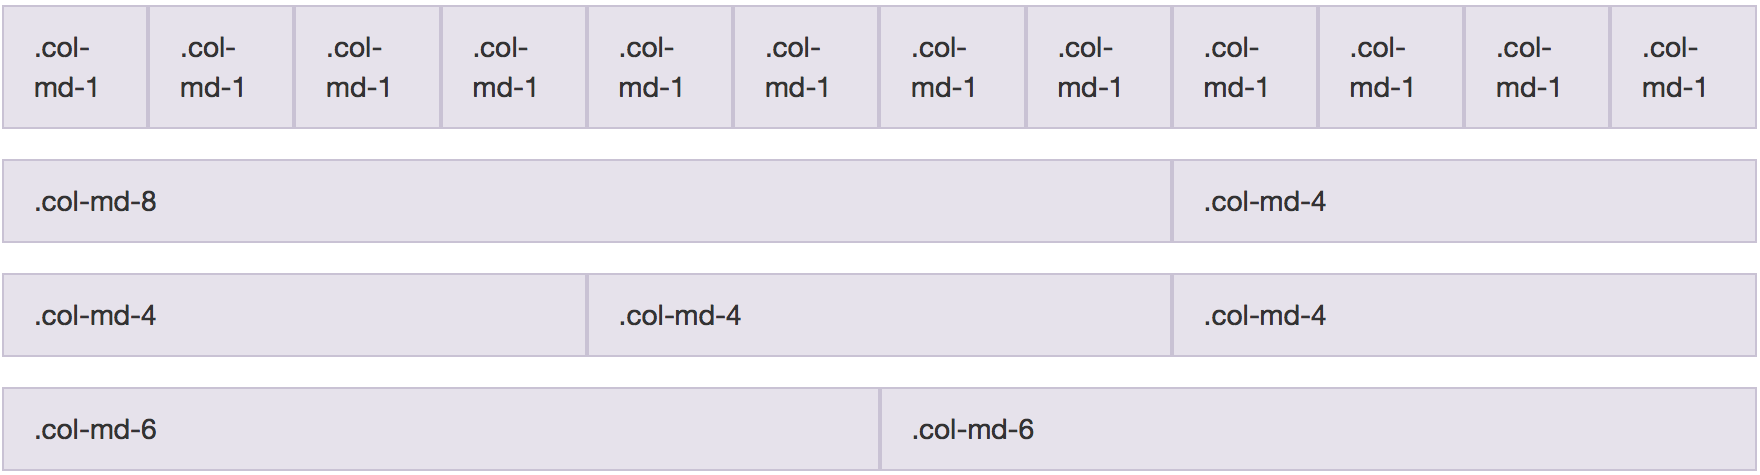
\includegraphics[width=1.0\textwidth]{images/Bootstrap_Grid}
	\caption{Bootstrap Responsive Grid Example} \label{fig:Bootstrap_Grid}
\end{figure}

The grid system works by using a series of rows and columns, where a row consists of 12 columns. A row is placed within a \emph{.container} or \emph{.container-fluid} for proper alignment. Content is placed within columns which can be different sized for different resolutions. Figure \ref{fig:Bootstrap_Grid} shows the grid system where the first row has 12 element of \emph{.col-md-1}, which means that on a medium size screen the columns will take up one column each, whereas the second row has two elements containing an element that is 8 columns wide and another which is only 4 columns wide. All these elements specify only column sizes for medium size screens but these are automatically cascaded to larger screens. However, on a screen size than is smaller than 'medium', the elements will each span 12 column and stack vertically. 

\begin{figure}[H]
	\centering
	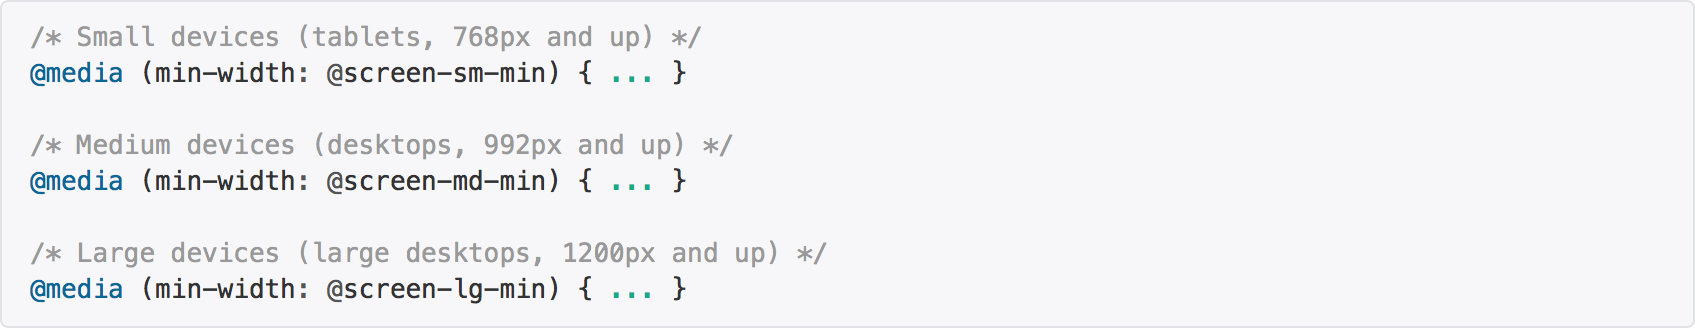
\includegraphics[width=1.0\textwidth]{images/Code/Media_Queries}
	\caption{Bootstrap Media Queries for Different Screen Sizes} \label{fig:Media_Queries}
\end{figure}

Figure \ref{fig:Media_Queries} shows the media queries used by bootstrap to achieve the functionality provided by the grid. Each of the classes is defined separately for each screen size inside the media queries. The grid layout was used throughout the entire website and all content was placed inside columns to ensure that it would be presented different only each device. However, this in itself was not enough as some content, such as the explore page which used absolute positioning, required custom styling. As a result, custom media queries had to be written to scale the content on these pages differently for each device. The CSS shown in figure \ref{fig:Grid_CSS} resizes the tile view on the explore page to 60\% on medium size screens but 100\% on smaller screen sizes.

\begin{figure}[H]
	\centering
	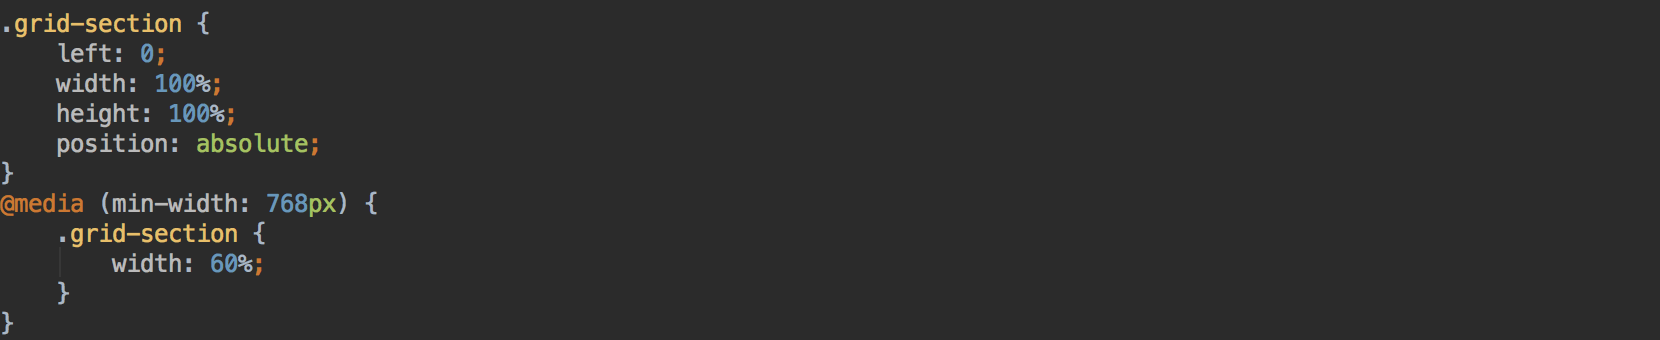
\includegraphics[width=1.0\textwidth]{images/Code/Grid_CSS}
	\caption{CSS for Changing Explore Layout Using Media Queries} \label{fig:Grid_CSS}
\end{figure}

Through the use of custom media queries, Bootstrap grid, and other CSS techniques, an entirely different experience was implemented for devices with different screen sizes. Figure \ref{fig:Mobile_View} shows the items page on the dashboard, search page, and the global navigation bar for pages in mobile view.

\begin{figure}[H]
	\centering
	\begin{subfigure}[t]{0.3\textwidth}
		\centering
		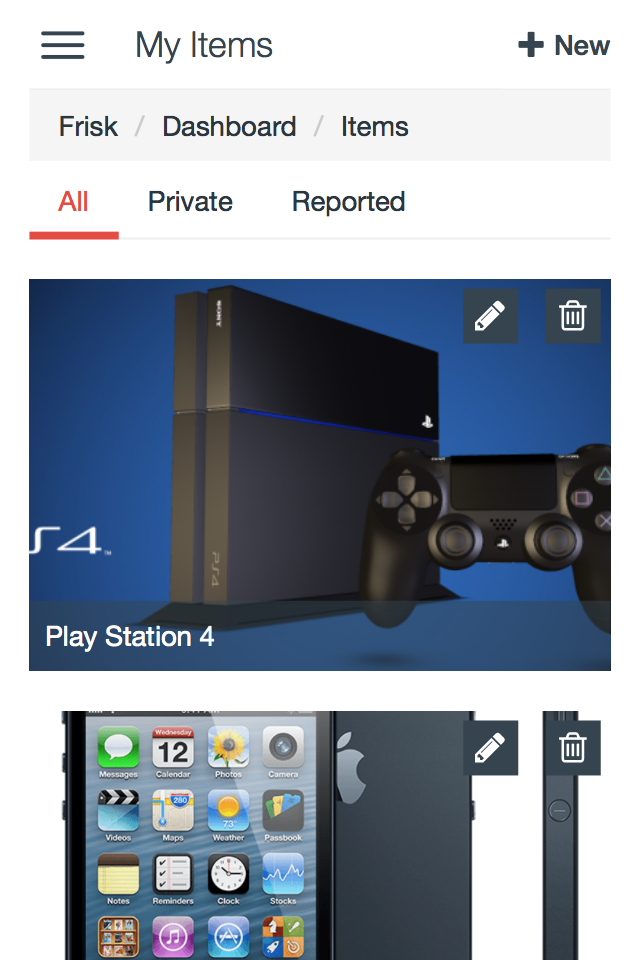
\includegraphics[width=1.0\textwidth]{images/Frisk/Mobile_Dashboard}
		\caption{Dashboard}\label{fig:Mobile_Dashboard}		
	\end{subfigure}
	\quad
	\begin{subfigure}[t]{0.3\textwidth}
		\centering
		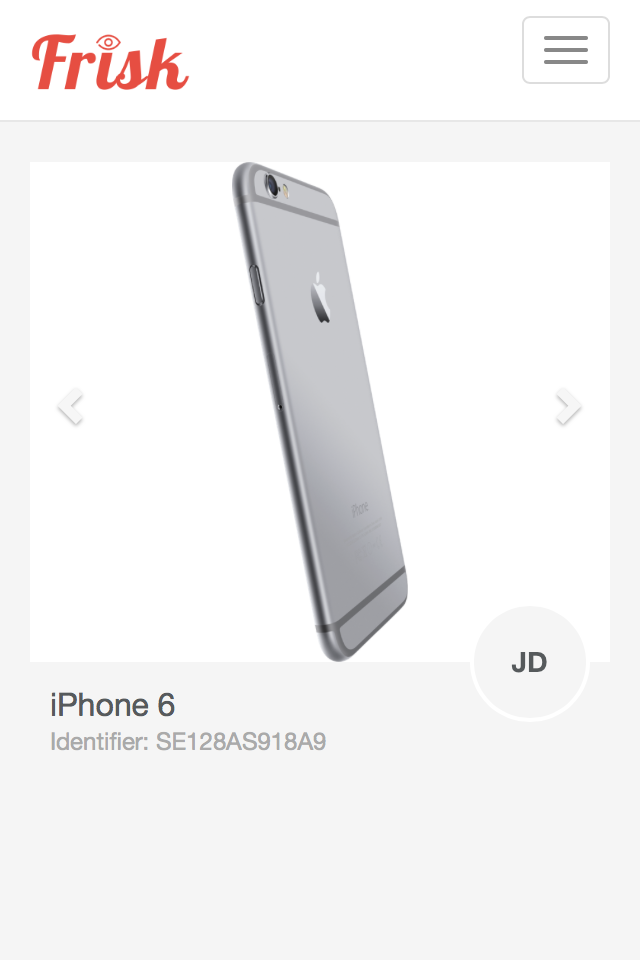
\includegraphics[width=1.0\textwidth]{images/Frisk/Mobile_Search}
		\caption{Search}\label{fig:Mobile_Search}
	\end{subfigure}
	\quad
	\begin{subfigure}[t]{0.3\textwidth}
		\centering
		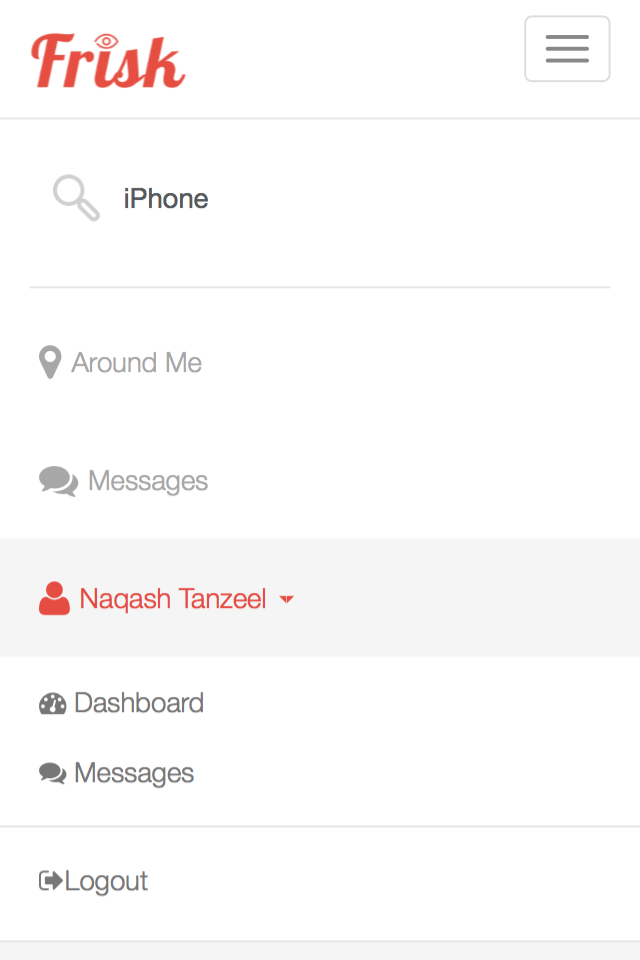
\includegraphics[width=1.0\textwidth]{images/Frisk/Mobile_Nav}
		\caption{Navigation}\label{fig:Mobile_Nav}
	\end{subfigure}
	\caption{Mobile Versions of Various Parts of the System}\label{fig:Mobile_View}
\end{figure}

\newpage